% !TeX spellcheck = en-US
% !TeX encoding = utf8
% !TeX program = pdflatex
% !BIB program = biber
% -*- coding:utf-8 mod:LaTeX -*-


% vv  scroll down to line 200 for content  vv


\let\ifdeutsch\iftrue
\let\ifenglish\iffalse


% EN: This file is loaded before the \documentclass command in the main document

% EN: The following package allows \\ at the title page
%     For more information see https://github.com/latextemplates/scientific-thesis-cover/issues/4
\RequirePackage{kvoptions-patch}

\ifenglisch
  \PassOptionsToClass{numbers=noenddot}{scrbook}
\else
  %()Aus scrguide.pdf - der Dokumentation von KOMA-Script)
  %Nach DUDEN steht in Gliederungen, in denen ausschließlich arabische Ziffern für die Nummerierung
  %verwendet werden, am Ende der Gliederungsnummern kein abschließender Punkt
  %(siehe [DUD96, R3]). Wird hingegen innerhalb der Gliederung auch mit römischen Zahlen
  %oder Groß- oder Kleinbuchstaben gearbeitet, so steht am Ende aller Gliederungsnummern ein
  %abschließender Punkt (siehe [DUD96, R4])
  \PassOptionsToClass{numbers=autoendperiod}{scrbook}
\fi

% Warns about outdated packages and missing caption declarations
% See https://www.ctan.org/pkg/nag
\RequirePackage[l2tabu, orthodox]{nag}

%DE: Neue deutsche Trennmuster
%    Siehe http://www.ctan.org/pkg/dehyph-exptl und http://projekte.dante.de/Trennmuster/WebHome
%    Nur für pdflatex, nicht für lualatex
\RequirePackage{ifluatex}
\ifluatex
  % do not load anything
\else
  \ifdeutsch
    \RequirePackage[ngerman=ngerman-x-latest]{hyphsubst}
  \fi
\fi

\documentclass[
  %
  %ngerman, %%% Add if you write in German.
  %
  % fontsize=11pt is the standard
  a4paper,  % Standard format - only KOMAScript uses paper=a4 - https://tex.stackexchange.com/a/61044/9075
  twoside,  % we are optimizing for both screen and two-side printing. So the page numbers will jump, but the content is configured to stay in the middle (by using the geometry package)
  bibliography=totoc,
  %               idxtotoc,   %Index ins Inhaltsverzeichnis
  %               liststotoc, %List of X ins Inhaltsverzeichnis, mit liststotocnumbered werden die Abbildungsverzeichnisse nummeriert
  headsepline,
  cleardoublepage=empty,
  parskip=half,
  %               draft    % um zu sehen, wo noch nachgebessert werden muss - wichtig, da Bindungskorrektur mit drin
  draft=false
]{scrbook}
% !TeX encoding = utf8
% -*- coding:utf-8 mod:LaTeX -*-

% EN: This file includes basic packages and sets options. The order of package
%     loading is important

% DE: In dieser Datei werden zuerst die benoetigten Pakete eingebunden und
%     danach diverse Optionen gesetzt. Achtung Reihenfolge ist entscheidend!


% EN: Styleguide:
% - English comments are prefixed with "EN", German comments are prefixed with "DE"
% - Prefixed headings define the language for the subsequent paragraphs
% - It is tried to organize packages in blocks. Bocks are separated by two empty lines.

% DE: Styleguide:
%
% Ein sehr kleiner Styleguide. Packages werden in Blöcken organisiert.
% Zwischen zwei Blöcken sind 2 Leerzeilen!


% EN: Enable copy and paste of text from the PDF
%     Only required for pdflatex. It "just works" in the case of lualatex.
%     mmap enables mathematical symbols, but does not work with the newtx font set
%     See: https://tex.stackexchange.com/a/64457/9075
%     Other solutions outlined at http://goemonx.blogspot.de/2012/01/pdflatex-ligaturen-und-copynpaste.html and http://tex.stackexchange.com/questions/4397/make-ligatures-in-linux-libertine-copyable-and-searchable
%     Trouble shooting outlined at https://tex.stackexchange.com/a/100618/9075

\ifluatex
\else
  \usepackage{cmap}
\fi


% EN: File encoding
% DE: Codierung
%     Wir sind im 21 Jahrhundert, utf-8 löst so viele Probleme.
%
% Mit UTF-8 funktionieren folgende Pakete nicht mehr. Bitte beachten!
%   * fancyvrb mit §
%   * easylist -> http://www.ctan.org/tex-archive/macros/latex/contrib/easylist/
\ifluatex
  % EN: See https://tex.stackexchange.com/a/158517/9075
  %     Not required, because of usage of fontspec package
  %\usepackage[utf8]{luainputenc}
\else
  \usepackage[utf8]{inputenc}
\fi


% DE: Parallelbetrieb tex4ht und pdflatex

\makeatletter
\@ifpackageloaded{tex4ht}{
  \def\iftex4ht{\iftrue}
}{
  \def\iftex4ht{\iffalse}
}
\makeatother


% EN: Mathematics
% DE: Mathematik
%
% DE: Viele Mathematik-Sachen. Siehe https://texdoc.net/pkg/amsmath
%
% EN: Options must be passed this way, otherwise it does not work with glossaries
% DE: fleqn (=Gleichungen linksbündig platzieren) funktioniert nicht direkt. Es muss noch ein Patch gemacht werden:
\PassOptionsToPackage{fleqn,leqno}{amsmath}
%
% DE: amsmath Muss nicht mehr geladen werden, da es von newtxmath automatisch geladen wird
% \usepackage{amsmath}


%% EN: Fonts
%% DE: Schriften
%%
%% !!! If you change the font, be sure that words such as "workflow" can
%% !!! still be copied from the PDF. If this is not the case, you have
%% !!! to use glyphtounicode. See comment at cmap package


% EN: Times Roman for all text
\ifluatex
  % source: Second proposed fix from the following answer: https://tex.stackexchange.com/a/394137
  \usepackage[no-math]{fontspec}
  \setmainfont{TeXGyreTermes-Regular}[
       BoldFont       = TeXGyreTermes-Bold ,
       ItalicFont     = TeXGyreTermes-Italic ,
       BoldItalicFont = TeXGyreTermes-BoldItalic,
       NFSSFamily     = ntxtlf]
  \setsansfont{TeX Gyre Heros Regular}[
       Scale=.9,
       BoldFont       = TeX Gyre Heros Bold,
       ItalicFont     = TeX Gyre Heros Italic,
       BoldItalicFont = TeX Gyre Heros BoldItalic]
  \setmonofont[StylisticSet={1,3},Scale=.9]{inconsolata}
  \RequirePackage{newtxmath}
\else
  \RequirePackage{newtxtext}
  \RequirePackage{newtxmath}
  % EN: looks good with times, but no equivalent for lualatex found,
  %     therefore replaced with inconsolata
  %\RequirePackage[zerostyle=b,scaled=.9]{newtxtt}
  \RequirePackage[varl,scaled=.9]{inconsolata}
\fi

% EN: Fallback font - if the subsequent font packages do not define a font (e.g., monospaced)
%     This is the modern package for "Computer Modern".
%     In case this gets activated, one has to switch from cmap package to glyphtounicode (in the case of pdflatex)
% DE: Fallback-Schriftart
%\usepackage[%
%    rm={oldstyle=false,proportional=true},%
%    sf={oldstyle=false,proportional=true},%
%    tt={oldstyle=false,proportional=true,variable=true},%
%    qt=false%
%]{cfr-lm}

% EN: Headings are typset in Helvetica (which is similar to Arial)
% DE: Schriftart fuer die Ueberschriften - ueberschreibt lmodern
%\usepackage[scaled=.95]{helvet}

% DE: Für Schreibschrift würde tun, muss aber nicht
%\usepackage{mathrsfs} %  \mathscr{ABC}

% EN: Font for the main text
% DE: Schriftart fuer den Fliesstext - ueberschreibt lmodern
%     Linux Libertine, siehe http://www.linuxlibertine.org/
%     Packageparamter [osf] = Minuskel-Ziffern
%     rm = libertine im Brottext, Linux Biolinum NICHT als serifenlose Schrift, sondern helvet (von oben) beibehalten
%\usepackage[rm]{libertine}

% EN: Alternative Font: Palantino. It is recommeded by Prof. Ludewig for German texts
% DE: Alternative Schriftart: Palantino, Packageparamter [osf] = Minuskel-Ziffern
%     Bitte nur in deutschen Texten
%\usepackage{mathpazo} %ftp://ftp.dante.de/tex-archive/fonts/mathpazo/ - Tipp aus DE-TEX-FAQ 8.2.1

% DE: Schriftart fuer Programmcode - ueberschreibt lmodern
%     Falls auskommentiert, wird die Standardschriftart lmodern genommen
%     Fuer schreibmaschinenartige Schluesselwoerter in den Listings - geht bei alten Installationen nicht, da einige Fontshapes (<>=) fehlen
%\usepackage[scaled=.92]{luximono}
%\usepackage{courier}
% DE: BeraMono als Typewriter-Schrift, Tipp von http://tex.stackexchange.com/a/71346/9075
%\usepackage[scaled=0.83]{beramono}

% EN: backticks (`) are rendered as such in verbatim environments.
%     See following links for details:
%     - https://tex.stackexchange.com/a/341057/9075
%     - https://tex.stackexchange.com/a/47451/9075
%     - https://tex.stackexchange.com/a/166791/9075
\usepackage{upquote}

% DE: Symbole
%
%\usepackage[geometry]{ifsym} % \BigSquare
%\usepackage{mathabx}
%\usepackage{stmaryrd} %fuer \ovee, \owedge, \otimes
%\usepackage{marvosym} %fuer \Writinghand %patched to not redefine \Rightarrow
%\usepackage{mathrsfs} %mittels \mathscr{} schoenen geschwungenen Buchstaben erzeugen
%\usepackage{calrsfs} %\mathcal{} ein bisserl dickeren buchstaben erzeugen - sieht net so gut aus.
%durch mathpazo ist das schon definiert

%
%\usepackage{amssymb}

% EN: For \texttrademark{}
\usepackage{textcomp}

% EN: name-clashes von marvosym und mathabx vermeiden:
\def\delsym#1{%
  %  \expandafter\let\expandafter\origsym\expandafter=\csname#1\endcsname
  %  \expandafter\let\csname orig#1\endcsname=\origsym
  \expandafter\let\csname#1\endcsname=\relax
}

%\usepackage{pifont}
%\usepackage{bbding}
%\delsym{Asterisk}
%\delsym{Sun}\delsym{Mercury}\delsym{Venus}\delsym{Earth}\delsym{Mars}
%\delsym{Jupiter}\delsym{Saturn}\delsym{Uranus}\delsym{Neptune}
%\delsym{Pluto}\delsym{Aries}\delsym{Taurus}\delsym{Gemini}
%\delsym{Rightarrow}
%\usepackage{mathabx} - Ueberschreibt leider zu viel - und die \le-Zeichen usw. sehen nicht gut aus!


% EN: Modern font encoding
%     Has to be loaded AFTER any font packages. See https://tex.stackexchange.com/a/2869/9075.
\ifluatex
\else
  \usepackage[T1]{fontenc}
\fi
%


% EN: Character protrusion and font expansion. See http://www.ctan.org/tex-archive/macros/latex/contrib/microtype/
% DE: Optischer Randausgleich und Grauwertkorrektur

\usepackage[
  babel=true, % EN: Enable language-specific kerning. Take language-settings from the languge of the current document (see Section 6 of microtype.pdf)
  expansion=alltext,
  protrusion=alltext-nott, % EN: Ensure that at listings, there is no change at the margin of the listing
  final % EN: Always enable microtype, even if in draft mode. This helps finding bad boxes quickly.
        %     In the standard configuration, this template is always in the final mode, so this option only makes a difference if "pros" use the draft mode
]{microtype}


% EN: \texttt{test -- test} keeps the "--" as "--" (and does not convert it to an en dash)
\DisableLigatures{encoding = T1, family = tt* }

% DE: fuer microtype
% DE: tracking=true muss als Parameter des microtype-packages mitgegeben werden
% DE: Deaktiviert, da dies bei Algorithmen seltsam aussieht

%\DeclareMicrotypeSet*[tracking]{my}{ font = */*/*/sc/* }%
%\SetTracking{ encoding = *, shape = sc }{ 45 }
% DE: Hier wird festgelegt,
%     dass alle Passagen in Kapitälchen automatisch leicht
%     gesperrt werden.
%     Quelle: http://homepage.ruhr-uni-bochum.de/Georg.Verweyen/pakete.html
%    Deaktiviert, da sonst "BPEL", "BPMN" usw. wirklich komisch aussehen.
%     Macht wohl nur bei geisteswissenschaftlichen Arbeiten Sinn.


% EN: amsmath teaks


% EN: Fixes bugs in AMS math
%     Corrently conflicts with unicode-math
% \usepackage{mathtools}

%\numberwithin{equation}{section}
%\renewcommand{\theequation}{\thesection.\Roman{equation}}

% EN: work-around ams-math problem with align and 9 -> 10. Does not work with glossaries, No visual changes.
%\addtolength\mathindent{1em}


% EN: For theorems, replacement for amsthm
\usepackage[amsmath,hyperref]{ntheorem}
\theorempreskipamount 2ex plus1ex minus0.5ex
\theorempostskipamount 2ex plus1ex minus0.5ex
\theoremstyle{break}
\newtheorem{definition}{Definition}[section]


% CTAN: https://ctan.org/pkg/lccaps
% Doc: http://texdoc.net/pkg/lccaps
%
% Required for DE/EN \initialism
\usepackage{lccaps}


% EN: Defintion of colors. Argument "hyperref" is not used as we do not want to change border colors of links: Links are not colored anymore.
% DE: Farbdefinitionen
\usepackage[dvipsnames]{xcolor}


% EN: Required for custom acronyms/glossaries style.
%     Left aligned Columns in tables with fixed width.
%     See http://tex.stackexchange.com/questions/91566/syntax-similar-to-centering-for-right-and-left
\usepackage{ragged2e}


% DE: Wichtig, ansonsten erscheint "No room for a new \write"
\usepackage{scrwfile}


% EN: Support for language-specific hyphenation
% DE: Neue deutsche Rechtschreibung und Literatur statt "Literature"
%     Die folgende Einstellung ist der Nachfolger von ngerman.sty
\ifdeutsch
  % DE: letzte Sprache ist default, Einbindung von "american" ermöglicht \begin{otherlanguage}{amercian}...\end{otherlanguage} oder \foreignlanguage{american}{Text in American}
  %     Siehe auch http://tex.stackexchange.com/a/50638/9075
  \usepackage[american,main=ngerman]{babel}
  % Ein "abstract" ist eine "Kurzfassung", keine "Zusammenfassung"
  \addto\captionsngerman{%
    \renewcommand\abstractname{Kurzfassung}%
  }
  \ifluatex
    % EN: conditionally disable ligatures. See https://github.com/latextemplates/scientific-thesis-template/issues/54
    %     for a discussion
    \usepackage[ngerman]{selnolig}
  \fi
\else
  % EN: Set English as language and allow to write hyphenated"=words
  %     `american`, `english` and `USenglish` are synonyms for babel package (according to https://tex.stackexchange.com/questions/12775/babel-english-american-usenglish).
  %      "english" has to go last to set it as default language
  \usepackage[english]{babel}
  % EN: Hint by http://tex.stackexchange.com/a/321066/9075 -> enable "= as dashes
  \addto\extrasenglish{\languageshorthands{ngerman}\useshorthands{"}}
  \ifluatex
    % EN: conditionally disable ligatures. See https://github.com/latextemplates/scientific-thesis-template/issues/54
    %     for a discussion
    \usepackage[english]{selnolig}
  \fi
\fi
%


% EN: For easy quotations: \enquote{text}
%     This package is very smart when nesting is applied, otherwise textcmds (see below) provides a shorter command
%     Note that this package results in a warning when it is loaded before minted (actually fvextra).
% DE: Anführungszeichen
%     Zitate in \enquote{...} setzen, dann werden automatisch die richtigen Anführungszeichen verwendet.
%     Dieses package erzeugt eine Warnung, wenn es vor minted (genauer fvextra) geladen wird.
\usepackage{csquotes}


% EN: For even easier quotations: \qq{text}.
%     Is not smart in the case of nesting, but good enough for the most cases
\usepackage{textcmds}
\ifdeutsch
  % EN: German quotes are different. So do not use the English quotes, but the ones provided by the csquotes package.
  \renewcommand{\qq}[1]{\enquote{#1}}
\fi


% EN: extended enumarations
% DE: erweitertes Enumerate
\usepackage{paralist}


% DE: Gestaltung der Kopf- und Fußteilen

\usepackage[automark]{scrlayer-scrpage}

\automark[section]{chapter}
\setkomafont{pageheadfoot}{\normalfont\sffamily}
\setkomafont{pagenumber}{\normalfont\sffamily}

% DE: funktioniert nicht: Alle Linien sind hier weg
%\setheadsepline[.4pt]{.4pt}


% DE: Intelligentes Leerzeichen um hinter Abkürzungen die richtigen Abstände zu erhalten, auch leere.
%     Siehe commands.tex \gq{}
\usepackage{xspace}
% DE: Macht \xspace und \enquote kompatibel
\makeatletter
\xspaceaddexceptions{\grqq \grq \csq@qclose@i \} }
\makeatother


\newcommand{\eg}{e.\,g.,\ }
\newcommand{\ie}{i.\,e.,\ }


% EN: introduce \powerset - hint by http://matheplanet.com/matheplanet/nuke/html/viewtopic.php?topic=136492&post_id=997377
\DeclareFontFamily{U}{MnSymbolC}{}
\DeclareSymbolFont{MnSyC}{U}{MnSymbolC}{m}{n}
\DeclareFontShape{U}{MnSymbolC}{m}{n}{
  <-6>    MnSymbolC5
  <6-7>   MnSymbolC6
  <7-8>   MnSymbolC7
  <8-9>   MnSymbolC8
  <9-10>  MnSymbolC9
  <10-12> MnSymbolC10
  <12->   MnSymbolC12%
}{}
\DeclareMathSymbol{\powerset}{\mathord}{MnSyC}{180}


% EN: Package for the appendix
% DE: Anhang
\usepackage{appendix}
%[toc,page,title,header]
%


% EN: Graphics
% DE: Grafikeinbindungen
%
% EN: The parameter "pdftex" is not required
\usepackage{graphicx}
\graphicspath{{\getgraphicspath}}
\newcommand{\getgraphicspath}{graphics/}


% EN: Enables inclusion of SVG graphics - 1:1 approach
%    This is NOT the approach of https://ctan.org/pkg/svg-inkscape,
%     which allows text in SVG to be typeset using LaTeX
%     We just include the SVG as is.
\usepackage{epstopdf}
\epstopdfDeclareGraphicsRule{.svg}{pdf}{.pdf}{%
  inkscape -z -D --file=#1 --export-pdf=\OutputFile
}


% EN: Enables inclusion of SVG graphics - text-rendered-with-LaTeX-approach
%     This is the approach of https://ctan.org/pkg/svg-inkscape,
\newcommand{\executeiffilenewer}[3]{%
  \IfFileExists{#2}
  {
    %\message{file #2 exists}
    \ifnum\pdfstrcmp{\pdffilemoddate{#1}}%
      {\pdffilemoddate{#2}}>0%
      {\immediate\write18{#3}}
    \else
      {%\message{file up to date #2}
      }
    \fi%
  }{
    %\message{file #2 doesn't exist}
    %\message{argument: #3}
    %\immediate\write18{echo "test" > xoutput.txt}
    \immediate\write18{#3}
  }
}
\newcommand{\includesvg}[1]{%
  \executeiffilenewer{#1.svg}{#1.pdf}%
  {
    inkscape -z -D --file=\getgraphicspath#1.svg %
    --export-pdf=\getgraphicspath#1.pdf --export-latex}%
  \input{\getgraphicspath#1.pdf_tex}%
}


% EN: Enable typesetting values with SI units.
%\ifdeutsch
%  \usepackage[mode=text,group-four-digits]{siunitx}
%  \sisetup{locale=DE}
%\else
%  \usepackage[mode=text,group-four-digits,group-separator={,}]{siunitx}
%  \sisetup{locale=US}
%\fi


% EN: Extensions for tables
% DE: Tabellenerweiterungen
\usepackage{array} %increases tex's buffer size and enables ``>'' in tablespecs
\usepackage{longtable}
\usepackage{dcolumn} %Aligning numbers by decimal points in table columns
\ifdeutsch
  \newcolumntype{d}[1]{D{.}{,}{#1}}
\else
  \newcolumntype{d}[1]{D{.}{.}{#1}}
\fi
\setlength{\extrarowheight}{1pt}


% DE: Eine Zelle, die sich über mehrere Zeilen erstreckt.
%     Siehe Beispieltabelle in Kapitel 2
\usepackage{multirow}


% DE: Fuer Tabellen mit Variablen Spaltenbreiten
\usepackage{tabularx}
%\usepackage{tabulary}


% EN: Links behave as they should. Enables "\url{...}" for URL typesettings.
%     Allow URL breaks also at a hyphen, even though it might be confusing: Is the "-" part of the address or just a hyphen?
%     See https://tex.stackexchange.com/a/3034/9075.
% DE: Links verhalten sich so, wie sie sollen
%     Zeilenumbrüche bei URLs auch bei Bindestrichen erlauben, auch wenn es verwirrend sein könnte: Gehört der Bindestrich zur URL oder ist es ein Trennstrich?
%     Siehe https://tex.stackexchange.com/a/3034/9075.
\usepackage[hyphens]{url}
%
%  EN: When activated, use text font as url font, not the monospaced one.
%      For all options see https://tex.stackexchange.com/a/261435/9075.
% \urlstyle{same}
%
% EN: Hint by http://tex.stackexchange.com/a/10419/9075.
\makeatletter
\g@addto@macro{\UrlBreaks}{\UrlOrds}
\makeatother


% DE: Index über Begriffe, Abkürzungen
%\usepackage{makeidx} makeidx ist out -> http://xindy.sf.net verwenden


% DE: lustiger Hack fuer das Abkuerzungsverzeichnis
%     nach latex durchlauf folgendes ausfuehren
%     makeindex ausarbeitung.nlo -s nomencl.ist -o ausarbeitung.nls
%     danach nochmal latex
%\usepackage{nomencl}
%    \let\abk\nomenclature %Deutsche Ueberschrift setzen
%          \renewcommand{\nomname}{List of Abbreviations}
%        %Punkte zw. Abkuerzung und Erklaerung
%          \setlength{\nomlabelwidth}{.2\hsize}
%          \renewcommand{\nomlabel}[1]{#1 \dotfill}
%        %Zeilenabstaende verkleinern
%          \setlength{\nomitemsep}{-\parsep}
%    \makenomenclature


% EN: Logic for TeX - enables if-then-else in commands
% DE: Logik für TeX
%     FÜr if-then-else @ commands.tex
\usepackage{ifthen}


% EN: Code Listings
% DE: Listings
\usepackage{listings}
\lstset{language=XML,
  showstringspaces=false,
  extendedchars=true,
  basicstyle=\footnotesize\ttfamily,
  commentstyle=\slshape,
  % DE: Original: \rmfamily, damit werden die Strings im Quellcode hervorgehoben. Zusaetzlich evtl.: \scshape oder \rmfamily durch \ttfamily ersetzen. Dann sieht's aus, wie bei fancyvrb
  stringstyle=\ttfamily,
  breaklines=true,
  breakatwhitespace=true,
  % EN: alternative: fixed
  columns=flexible,
  numbers=left,
  numberstyle=\tiny,
  basewidth=.5em,
  xleftmargin=.5cm,
  % aboveskip=0mm, %DE: deaktivieren, falls man lstlistings direkt als floating object benutzt (\begin{lstlisting}[float,...])
  % belowskip=0mm, %DE: deaktivieren, falls man lstlistings direkt als floating object benutzt (\begin{lstlisting}[float,...])
  captionpos=b
}

\ifluatex
\else
  % EN: Enable UTF-8 support - see https://tex.stackexchange.com/q/419327/9075
  \usepackage{listingsutf8}
  \lstset{inputencoding=utf8/latin1}
\fi

\ifdeutsch
  \renewcommand{\lstlistlistingname}{Verzeichnis der Listings}
\fi


% EN: Alternative to listings could be fancyvrb. Can be used together.
% DE: Alternative zu Listings ist fancyvrb. Kann auch beides gleichzeitig benutzt werden.
\usepackage{fancyvrb}
%
% EN: Font size for the normal text
% DE: Groesse fuer den Fliesstext. Falls deaktiviert: \normalsize
%\fvset{fontsize=\small}
%
% DE: Somit kann im Text ganz einfach §verbatim§ text gesetzt werden.
%     Disabled, because UTF-8 does not work any more and lualatex causes issues
%\DefineShortVerb{\§}
%
% EN: Shrink font size of listings
\RecustomVerbatimEnvironment{Verbatim}{Verbatim}{fontsize=\footnotesize}
\RecustomVerbatimCommand{\VerbatimInput}{VerbatimInput}{fontsize=\footnotesize}
%
% EN: Hack for fancyvrb based on http://newsgroups.derkeiler.com/Archive/Comp/comp.text.tex/2008-12/msg00075.html
%     Change of the solution: \Vref somehow collidated with cleveref/varioref as the output of \Vref{} was "Abschnitt 4.3 auf Seite 85"; therefore changed to \myVref -- so completely removed
%     See https://tex.stackexchange.com/q/132420/9075 for more information.
\newcommand{\Vlabel}[1]{\label[line]{#1}\hypertarget{#1}{}}
\newcommand{\lref}[1]{\hyperlink{#1}{\FancyVerbLineautorefname~\ref*{#1}}}


% EN: Tunings of captions for floats, listings, ...
% DE: Bildunterschriften bei floats genauso formatieren wie bei Listings
%     Anpassung wird unten bei den newfloat-Deklarationen vorgenommen
%     https://www.ctan.org/pkg/caption2 is superseeded by this package.
\usepackage{caption}


% EN: Provides rotating figures, where the PDF page is also turned
% DE: Ermoeglicht es, Abbildungen um 90 Grad zu drehen
%     Alternatives Paket: rotating Allerdings wird hier nur das Bild gedreht, während bei lscape auch die PDF-Seite gedreht wird.
%     Das Paket lscape dreht die Seite auch nicht
\usepackage{pdflscape}


% EN: Required for proper environments of fancyvrb and lstlistings
%    There is also the newfloat pacakge (recommended by minted), but we currently have no expericene with that
% DE: Wird für fancyvrb und für lstlistings verwendet
\usepackage{float}
%
% EN: Alternative to float package
%\usepackage{floatrow}
% DE: zustäzlich für den Paramter [H] = Floats WIRKLICH da wo sie deklariert wurden paltzieren - ganz ohne Kompromisse
%     floatrow ist der Nachfolger von float
%     Allerdings macht floatrow in manchen Konstellationen Probleme. Deshalb ist das Paket deaktiviert.
%
% EN: See http://www.tex.ac.uk/cgi-bin/texfaq2html?label=floats
% DE: floats IMMER nach einer Referenzierung platzieren
%\usepackage{flafter}


% EN: Put footnotes below floats
%     Source: https://tex.stackexchange.com/a/32993/9075
\usepackage{stfloats}
\fnbelowfloat


% EN: For nested figures
% DE: Fuer Abbildungen innerhalb von Abbildungen
%     Ersetzt die Pakete subfigure und subfig - siehe https://tex.stackexchange.com/a/13778/9075
\usepackage[hypcap=true]{subcaption}


% EN: Extended support for footnotes
% DE: Fußnoten
%
%\usepackage{dblfnote}  %Zweispaltige Fußnoten
%
% Keine hochgestellten Ziffern in der Fußnote (KOMA-Script-spezifisch):
%\deffootnote[1.5em]{0pt}{1em}{\makebox[1.5em][l]{\bfseries\thefootnotemark}}
%
% Abstand zwischen Fußnoten vergrößern:
%\setlength{\footnotesep}{.85\baselineskip}
%
% EN: Following command disables the separting line of the footnote
% DE: Folgendes Kommando deaktiviert die Trennlinie zur Fußnote
%\renewcommand{\footnoterule}{}
%
\addtolength{\skip\footins}{\baselineskip} % Abstand Text <-> Fußnote
%
% Fußnoten immer ganz unten auf einer \raggedbottom-Seite
% fnpos kommt aus dem yafoot package
\usepackage{fnpos}
\makeFNbelow
\makeFNbottom


% EN: Variable page heights
% DE: Variable Seitenhöhen zulassen
\raggedbottom


% DE: Falls die Seitenzahl bei einer Referenz auf eine Abbildung nur dann angegeben werden soll,
%     falls sich die Abbildung nicht auf der selben Seite befindet...
\iftex4ht
  %tex4ht does not work well with vref, therefore we emulate vref behavior
  \newcommand{\vref}[1]{\ref{#1}}
\else
  \ifdeutsch
    \usepackage[ngerman]{varioref}
  \else
    \usepackage{varioref}
  \fi
\fi


% EN: More beautiful tables if one uses \toprule, \midrule, \bottomrule
% DE: Noch schoenere Tabellen als mit booktabs mit http://www.zvisionwelt.de/downloads.html
\usepackage{booktabs}
%
%\usepackage[section]{placeins}


% EN: Graphs and Automata
%
% TODO: Since version 3.0 (2013-10-01), it supports pdflatex via the auto-pst-pdf package
%       Requires -shell-escape
%\usepackage{gastex}


%\usepackage{multicol}

% DE: kollidiert mit diplomarbeit.sty
%\usepackage{setspace}


% DE: biblatex statt bibtex
\usepackage[
  backend       = biber, %biber does not work with 64x versions alternative: bibtex8
  %minalphanames only works with biber backend
  sortcites     = true,
  bibstyle      = numeric,
  citestyle     = numeric,
  giveninits    = false,
  useprefix     = false, %"von, van, etc." will be printed, too. See below.
  minnames      = 1,
  minalphanames = 3,
  maxalphanames = 4,
  maxbibnames   = 99,
  maxcitenames  = 2,
  natbib        = true,
  eprint        = true,
  url           = true,
  doi           = true,
  isbn          = true,
  backref       = false]{biblatex}

% enable more breaks at URLs. See https://tex.stackexchange.com/a/134281.
\setcounter{biburllcpenalty}{7000}
\setcounter{biburlucpenalty}{8000}

\bibliography{bibliography}
\addbibresource[datatype=bibtex]{bibliography.bib}

%Do not put "vd" in the label, but put it at "\citeauthor"
%Source: http://tex.stackexchange.com/a/30277/9075
\makeatletter
\AtBeginDocument{\toggletrue{blx@useprefix}}
\AtBeginBibliography{\togglefalse{blx@useprefix}}
\makeatother

%Thin spaces between initials
%http://tex.stackexchange.com/a/11083/9075
\renewrobustcmd*{\bibinitdelim}{\,}

%Keep first and last name together in the bibliography
%http://tex.stackexchange.com/a/196192/9075
\renewcommand*\bibnamedelimc{\addnbspace}
\renewcommand*\bibnamedelimd{\addnbspace}

%Replace last "and" by comma in bibliography
%See http://tex.stackexchange.com/a/41532/9075
\AtBeginBibliography{%
  \renewcommand*{\finalnamedelim}{\addcomma\space}%
}

\ifdeutsch
  \DefineBibliographyStrings{ngerman}{
    backrefpage  = {zitiert auf S\adddot},
    backrefpages = {zitiert auf S\adddot},
    andothers    = {et\ \addabbrvspace al\adddot},
    %Tipp von http://www.mrunix.de/forums/showthread.php?64665-biblatex-Kann-%DCberschrift-vom-Inhaltsverzeichnis-nicht-%E4ndern&p=293656&viewfull=1#post293656
    bibliography = {Literaturverzeichnis}
  }
\fi

% EN: enable hyperlinked author names when using \citeauthor
%     source: http://tex.stackexchange.com/a/75916/9075
\DeclareCiteCommand{\citeauthor}
{\boolfalse{citetracker}%
  \boolfalse{pagetracker}%
  \usebibmacro{prenote}}
{\ifciteindex
  {\indexnames{labelname}}
  {}%
  \printtext[bibhyperref]{\printnames{labelname}}}
{\multicitedelim}
{\usebibmacro{postnote}}

% EN: natbib compatibility
%\newcommand{\citep}[1]{\cite{#1}}
%\newcommand{\citet}[1]{\citeauthor{#1} \cite{#1}}
% EN: Beginning of sentence - analogous to cleveref - important for names such as "zur Muehlen"
%\newcommand{\Citep}[1]{\cite{#1}}
%\newcommand{\Citet}[1]{\Citeauthor{#1} \cite{#1}}

% DE: Blindtext. Paket "blindtext" ist fortgeschritterner als "lipsum" und kann auch Mathematik im Text (http://texblog.org/2011/02/26/generating-dummy-textblindtext-with-latex-for-testing/)
%     kantlipsum (https://www.ctan.org/tex-archive/macros/latex/contrib/kantlipsum) ist auch ganz nett, aber eben auch keine Mathematik
%     Wird verwendet, um etwas Text zu erzeugen, um eine volle Seite wegen Layout zu sehen.
\usepackage[math]{blindtext}


% EN: Make LaTeX logos available by commands. E.g., \lualatex
%     Disabled, because currently causes \not= already defined
%\usepackage{dtk-logos}

% quick replacement:
\newcommand{\LuaLaTeX}{Lua\LaTeX\xspace}
\newcommand{\lualatex}{\LuaLaTeX}

% DE: Neue Pakete bitte VOR hyperref einbinden. Insbesondere bei Verwendung des
%     Pakets "index" wichtig, da sonst die Referenzierung nicht funktioniert.
%     Für die Indizierung selbst ist unter http://xindy.sourceforge.net
%     ein gutes Tool zu erhalten.
%     Hier also neue packages einbinden.
% EN: Add new packages at this place.


% EN: Provides hyperlinks
%     Option "unicode" fixes umlauts in the PDF bookmarks - see https://tex.stackexchange.com/a/338770/9075
%
% DE: Erlaubt Hyperlinks im Dokument.
%     Alle Optionen nach \hypersetup verschoben, sonst crash
%     Siehe auch: "Praktisches LaTeX" - www.itp.uni-hannover.de/~kreutzm
\usepackage[unicode]{hyperref}


% EN: Define colors
% DE: Da es mit KOMA 3 und xcolor zu Problemen mit den global Options kommt MÜSSEN die Optionen so gesetzt werden.
%     Eigene Farbdefinitionen ohne die Namen des xcolor packages
\definecolor{darkblue}{rgb}{0,0,.5}
\definecolor{black}{rgb}{0,0,0}


% EN: Define color of links and more
\hypersetup{
  % have both title and number hyperlinking to content
  linktoc=all,
  bookmarksnumbered=true,
  bookmarksopen=true,
  bookmarksopenlevel=1,
  breaklinks=true,
  colorlinks=true,
  pdfstartview=Fit,
  pdfpagelayout=SinglePage, % DE: Alterntaive: TwoPageRight -- zweiseitige Darstellung: ungerade Seiten rechts im PDF-Viewer - siehe auch http://tex.stackexchange.com/a/21109/9075
  %pdfencoding=utf8, % EN: This is probably the same as passing the option "unicode" at \usepackage{hyperref}
  filecolor=black,
  urlcolor=black,
  linkcolor=black,
  citecolor=black
}

\ifenglish
    %\renewcommand{\sectionautorefname}{Section}
    %\renewcommand{\subsectionautorefname}{Section}
    %\renewcommand{\subsubsectionautorefname}{Section}
    \defcaptionname*{english}{\chapterautorefname}{Chapter}
    \defcaptionname*{english}{\sectionautorefname}{Section}
    \defcaptionname*{english}{\subsectionautorefname}{Section}
    \defcaptionname*{english}{\subsubsectionautorefname}{Section}
    \defcaptionname*{english}{\Listingautorefname}{Listing}
    \defcaptionname*{english}{\Algorithmusautorefname}{Algorithmus}
\else
\fi

% EN: Abbreviations - has to be loaded after hyperref
% DE: Abkürzungsverzeichnis - muss nach hyperref geladen werden
%
% DE: siehe http://www.dickimaw-books.com/cgi-bin/faq.cgi?action=view&categorylabel=glossaries#glsnewwriteexceeded
\usepackage[acronym,indexonlyfirst,nomain]{glossaries}
\ifdeutsch
  \addto\captionsngerman % DE: siehe https://tex.stackexchange.com/a/154566
  {%
    \renewcommand*{\acronymname}{Abkürzungsverzeichnis}
  }
\else
  \renewcommand*{\acronymname}{List of Abbreviations}
\fi
\renewcommand*{\glsgroupskip}{}
%
% EN: Removed Glossarie as a table as a quick fix to get the template working again
%     See http://tex.stackexchange.com/questions/145579/how-to-print-acronyms-of-glossaries-into-a-table
%
\makenoidxglossaries


% EN: Extensions for references inside the document (\cref{fig:sample}, ...)
% DE: cleveref für cref statt autoref, da cleveref auch bei Definitionen funktioniert
%\usepackage[capitalise,nameinlink,noabbrev]{cleveref}
%\ifdeutsch
%  \crefname{table}{Tabelle}{Tabellen}
%  \Crefname{table}{Tabelle}{Tabellen}
%  \crefname{figure}{\figurename}{\figurename}
%  \Crefname{figure}{Abbildung}{Abbildungen}
%  \crefname{equation}{Gleichung}{Gleichungen}
%  \Crefname{equation}{Gleichung}{Gleichungen}
%  \crefname{theorem}{Theorem}{Theoreme}
%  \Crefname{theorem}{Theorem}{Theoreme}
%  \crefname{listing}{\lstlistingname}{\lstlistingname}
%  \Crefname{listing}{Listing}{Listings}
%  \crefname{section}{Abschnitt}{Abschnitte}
%  \Crefname{section}{Abschnitt}{Abschnitte}
%  \crefname{paragraph}{Abschnitt}{Abschnitte}
%  \Crefname{paragraph}{Abschnitt}{Abschnitte}
%  \crefname{subparagraph}{Abschnitt}{Abschnitte}
%  \Crefname{subparagraph}{Abschnitt}{Abschnitte}
%\else
%  \crefname{listing}{\lstlistingname}{\lstlistingname}
%  \Crefname{listing}{Listing}{Listings}
%\fi


% DE: Zur Darstellung von Algorithmen
%     Algorithm muss nach hyperref geladen werden
\usepackage[chapter]{algorithm}
\usepackage[]{algpseudocode}


% DE: Links auf Gleitumgebungen springen nicht zur Beschriftung,
%     Doc: http://mirror.ctan.org/tex-archive/macros/latex/contrib/oberdiek/hypcap.pdf
%     sondern zum Anfang der Gleitumgebung
\usepackage[all]{hypcap}


% DE: Deckblattstyle
%
\ifdeutsch
  \PassOptionsToPackage{language=german}{scientific-thesis-cover}
\else
  \PassOptionsToPackage{language=english}{scientific-thesis-cover}
\fi


% EN: Bugfixes packages
%\usepackage{fixltx2e} %Fuer neueste LaTeX-Installationen nicht mehr benoetigt - bereinigte einige Ungereimtheiten, die auf Grund von Rueckwaertskompatibilitaet beibahlten wurden.
%\usepackage{mparhack} %Fixt die Position von marginpars (die in DAs selten bis gar nicht gebraucht werden}
%\usepackage{ellipsis} %Fixt die Abstaende vor \ldots. Wird wohl auch nicht benoetigt.


% EN: Settings for captions of floats
% DE: Formatierung der Beschriftungen
%
\captionsetup{
  format=hang,
  labelfont=bf,
  justification=justified,
  %single line captions should be centered, multiline captions justified
  singlelinecheck=true
}


% EN: New float environments for listings and algorithms
%
% \floatstyle{ruled} % TODO: enabled or disabled causes no change - listings and algorithms are always ruled
%
\newfloat{Listing}{tbp}{code}[chapter]
%\crefname{Listing}{Listing}{Listings}

\newfloat{Algorithmus}{tbp}{alg}[chapter]
\ifdeutsch
  %\crefname{Algorithmus}{Algorithmus}{Algorithmus}
\else
  %\crefname{Algorithmus}{Algorithm}{Algorithms}
  \floatname{Algorithmus}{Algorithm}
\fi



% EN: Various chapter styles
% DE: unterschiedliche Chapter-Styles
%     u.a. Paket fncychap

% Andere Kapitelueberschriften
% falls einem der Standard von KOMA nicht gefaellt...
% Falls man zurück zu KOMA moechte, dann muss jede der vier folgenden Moeglichkeiten deaktiviert sein.

%\usepackage[Sonny]{fncychap}

%\usepackage[Bjarne]{fncychap}

%\usepackage[Lenny]{fncychap}

%DE: Zur Aktivierung eines der folgenden Möglichkeiten ein Paar von "\iffalse" und "\fi" auskommentieren

\iffalse
  \usepackage[Bjarne]{fncychap}
  \ChNameVar{\Large\sf} \ChNumVar{\Huge} \ChTitleVar{\Large\sf}
  \ChRuleWidth{0.5pt} \ChNameUpperCase
\fi

\iffalse
  \usepackage[Rejne]{fncychap}
  \ChNameVar{\centering\Huge\rm\bfseries}
  \ChNumVar{\Huge}
  \ChTitleVar{\centering\Huge\rm}
  \ChNameUpperCase
  \ChTitleUpperCase
  \ChRuleWidth{1pt}
\fi

\iffalse
  \usepackage{fncychap}
  \ChNameUpperCase
  \ChTitleUpperCase
  \ChNameVar{\raggedright\normalsize} %\rm
  \ChNumVar{\bfseries\Large}
  \ChTitleVar{\raggedright\Huge}
  \ChRuleWidth{1pt}
\fi

\iffalse
  \usepackage[Bjornstrup]{fncychap}
  \ChNumVar{\fontsize{76}{80}\selectfont\sffamily\bfseries}
  \ChTitleVar{\raggedright\Large\sffamily\bfseries}
\fi

% EN: Complete different chapter style - self made

% Innen drin kann man dann noch zwischen
%   * serifenloser Schriftart (eingestellt)
%   * serifenhafter Schriftart (wenn kein zusaetzliches Kommando aktiviert ist) und
%   * Kapitälchen wählen
\iffalse
  \makeatletter
  %\def\thickhrulefill{\leavevmode \leaders \hrule height 1ex \hfill \kern \z@}

  %Fuer Kapitel mit Kapitelnummer
  \def\@makechapterhead#1{%
    \vspace*{10\p@}%
    {\parindent \z@ \raggedright \reset@font
      %Default-Schrift: Serifenhaft (gut fuer englische Dokumente)
      %A) Fuer serifenlose Schrift:
      \fontfamily{phv}\selectfont
      %B) Fuer Kapitaelchen:
      %\fontseries{m}\fontshape{sc}\selectfont
      %C) Fuer ganz "normale" Schrift:
      %\normalfont
      %
      \Large \@chapapp{} \thechapter
      \par\nobreak\vspace*{10\p@}%
      \interlinepenalty\@M
      {\Huge\bfseries\baselineskip3ex
        %Fuer Kapitaelchen folgende Zeile aktivieren:
        %\fontseries{m}\fontshape{sc}\selectfont
        #1\par\nobreak}
      \vspace*{10\p@}%
      \makebox[\textwidth]{\hrulefill}%    \hrulefill alone does not work
      \par\nobreak
      \vskip 40\p@
    }}

  %Fuer Kapitel ohne Kapitelnummer (z.B. Inhaltsverzeichnis)
  \def\@makeschapterhead#1{%
    \vspace*{10\p@}%
    {\parindent \z@ \raggedright \reset@font
      \normalfont \vphantom{\@chapapp{} \thechapter}
      \par\nobreak\vspace*{10\p@}%
      \interlinepenalty\@M
      {\Huge \bfseries %
        %Default-Schrift: Serifenhaft (gut fuer englische Dokumente)
        %A) Fuer serifenlose Schrift folgende Zeile aktivieren:
        \fontfamily{phv}\selectfont
        %B) Fuer Kapitaelchen folgende Zeile aktivieren:
        %\fontseries{m}\fontshape{sc}\selectfont
        #1\par\nobreak}
      \vspace*{10\p@}%
      \makebox[\textwidth]{\hrulefill}%    \hrulefill does not work
      \par\nobreak
      \vskip 40\p@
    }}
  %
  \makeatother
\fi


% DE: Minitoc-Einstellungen
%\dominitoc
%\renewcommand{\mtctitle}{Inhaltsverzeichnis dieses Kapitels}


% EN: Nicer paragraph line placement:
%     - Disable single lines at the start of a paragraph (Schusterjungen)
%     - Disable single lines at the end of a paragraph (Hurenkinder)
%     Normally, this is clubpenalty and widowpenalty, but using a package, it feels more non-hacky
\usepackage[all,defaultlines=3]{nowidow}
%
\displaywidowpenalty = 10000


% EN: Try to get rid of "overfull hbox" things and let text flow batter
%     See also
%       - http://groups.google.de/group/de.comp.text.tex/browse_thread/thread/f97da71d90442816/f5da290593fd647e?lnk=st&q=tolerance+emergencystretch&rnum=5&hl=de#f5da290593fd647e
%       - http://www.tex.ac.uk/cgi-bin/texfaq2html?label=overfull
\tolerance=2000
%
% EN: This could be increased to 20pt
\setlength{\emergencystretch}{3pt}
%
% EN: Suppress hbox warnings if less than 1pt
\setlength{\hfuzz}{1pt}


% EN: Fix names for algorithms in German
% DE: fuer algorithm.sty: - falls Deutsch und nicht Englisch.
\ifdeutsch
  \floatname{algorithm}{Algorithmus}
  \renewcommand{\listalgorithmname}{Verzeichnis der Algorithmen}
\fi


% EN: The euro sign
% DE: Das Euro Zeichen
%     Fuer Palatino (mathpazo.sty): richtiges Euro-Zeichen
%     Alternative: \usepackage{eurosym}
\newcommand{\EUR}{\ppleuro}


% Float-placements - http://dcwww.camd.dtu.dk/~schiotz/comp/LatexTips/LatexTips.html#figplacement
% and http://people.cs.uu.nl/piet/floats/node1.html
\renewcommand{\topfraction}{0.85}
\renewcommand{\bottomfraction}{0.95}
\renewcommand{\textfraction}{0.1}
\renewcommand{\floatpagefraction}{0.75}
%\setcounter{totalnumber}{5}

% EN: ensure that floats covering a whole page are placed at the top of the page
%    see http://tex.stackexchange.com/a/28565/9075
\makeatletter
\setlength{\@fptop}{0pt}
\setlength{\@fpbot}{0pt plus 1fil}
\makeatother



% DE: Bei Gleichungen nur dann die Nummer zeigen, wenn die Gleichung auch referenziert wird
%     Funktioniert mit MiKTeX Stand 2012-01-13 nicht. Deshalb ist dieser Schalter deaktiviert.
%
%\mathtoolsset{showonlyrefs}


% EN: Margins
% DE: Ränder
%     Viele Moeglichkeiten, die Raender im Dokument einzustellen.
%
%     Satzspiegel neu berechnen. Dokumentation dazu ist in "scrguide.pdf" von KOMA-Skript zu finden
%     Optionen werden bei \documentclass[] in ausarbeitung.tex mitgegeben.
% \typearea[current]{current} %neu berechnen, da neue Schrift eingebunden

%\usepackage{a4}
%\usepackage{a4wide}
%\areaset{170mm}{277mm} %a4:29,7hochx21mbreit

%Wer die Masse direkt eingeben moechte:
%Bei diesem Beispiel wird die Regel nicht beachtet, dass der innere Rand halb so gross wie der aussere Rand und der obere Rand halb so gross wie der untere Rand sein sollte
%\usepackage[inner=2.5cm, outer=2.5cm, includefoot, top=3cm, bottom=1.5cm]{geometry}

% EN: Package geometry to enlarge on page
%
%     Normally, geometry should not be used as the typearea package calculates the margins perfectly for printing
%     However, we want better screen-readable documents where the content does not "jump"
%     Thus, we fix the margins left and right to the same value
%
%     Source: http://www.howtotex.com/tips-tricks/change-margins-of-a-single-page/
%
\usepackage[
  left=3cm,right=3cm,top=2.5cm,bottom=2.5cm,
  headsep=18pt,
  footskip=30pt,
  includehead,
  includefoot
]{geometry}


% EN: Provides todo notes
% DE: schoene TODOs
\ifdeutsch
  \usepackage[colorinlistoftodos,ngerman]{todonotes}
\else
  \usepackage[colorinlistoftodos]{todonotes}
\fi
\setlength{\marginparwidth}{2,5cm}

\let\xtodo\todo
\renewcommand{\todo}[1]{\xtodo[inline,color=black!5]{#1}}
\newcommand{\utodo}[1]{\xtodo[inline,color=green!5]{#1}}
\newcommand{\itodo}[1]{\xtodo[inline]{#1}}


% EN: Enable footnotes in tables.
%     This package superseeds the 1997 package "footnote"
\usepackage{footnotehyper}
% TODO: The footnotehyper author recommends to enclose the respective area with \begin{savenotes} ... \end{savenotes}
\makesavenoteenv{tabular}
\makesavenoteenv{table}
% Reuse of footnotes, see http://tex.stackexchange.com/questions/10102/multiple-references-to-the-same-footnote-with-hyperref-support-is-there-a-bett
%\crefformat{footnote}{#2\footnotemark[#1]#3}


% EN: pgfplots (optional if the ppackage is installed)
%     PGFPlots draws high-qual­ity func­tion plots in nor­mal or log­a­rith­mic scal­ing
\IfFileExists{pgfplots.sty}{
  \usepackage{pgfplots}
  % EN: highest version supported by overleaf as of 2018-03-16
  \pgfplotsset{compat=1.14}
}{}


% EN: pgfplotstable (optional if the ppackage is installed)
%     PGFPlots generates tables from csv files
\IfFileExists{pgfplotstable.sty}{
  \usepackage{pgfplotstable}
}{}


% EN: Package for creating graphics programmatically
\usepackage{tikz}


% EN: Package for creating uml diagramms
\usepackage{tikz-uml}


% EN: Forest: apgf/TikZ-based package for drawing linguistic trees - https://ctan.org/pkg/forest
\usepackage{forest}


% EN: Enable PlantUML listings in the environment "plantuml"
\IfFileExists{plantuml.sty}{
  \usepackage[output=latex]{plantuml}
}{}


% EN: Layout: bottoms of pages not aligned to each other
% DE: Der untere Rand darf "flattern"
\raggedbottom


% DE: Wie tief wird das Inhaltsverzeichnis aufgeschlüsselt
% 0 --\chapter
% 1 --\section % fuer kuerzeres Inhaltsverzeichnis verwenden - oder minitoc benutzen
% 2 --\subsection
% 3 --\subsubsection
% 4 --\paragraph
\setcounter{tocdepth}{1}


% EN: Fixes wrong spacing in the TOC.
%     Source: https://tex.stackexchange.com/a/33842/9075 -> comment by esdd
\RedeclareSectionCommand[tocnumwidth=2.8em]{section}

% Fix TOC sans serif font -- https://tex.stackexchange.com/questions/625079/how-to-control-font-in-srcbook-koma-script-table-of-contents
\RedeclareSectionCommands[%
  tocentrynumberformat=\sffamily,%
  tocentryformat=\sffamily,%
  tocpagenumberformat=\sffamily,%
]{section}

\RedeclareSectionCommands[%
  tocentrynumberformat=\sffamily,%
  tocentryformat=\sffamily,%
  tocpagenumberformat=\sffamily,%
]{subsection}

\RedeclareSectionCommands[%
  tocentrynumberformat=\sffamily,%
  tocentryformat=\sffamily,%
  tocpagenumberformat=\sffamily,%
]{subsubsection}


% DE: Angaben in die PDF-Infos uebernehmen
\makeatletter
\hypersetup{
  pdftitle={}, %Titel der Arbeit
  pdfauthor={}, %Author
  pdfkeywords={}, % CR-Klassifikation und ggf. weitere Stichworte
  pdfsubject={}
}
\makeatother


% EN: Higher compression of the output PDF
\pdfcompresslevel=9


% EN: Required for recent version of komascript, as some packges are not that compatible with KOMAScript as they should be
%     Has to be loaded at the *very* end, so we use "\AtEndPreamble" by etoolsbox
\usepackage{etoolbox}
\AtEndPreamble{\usepackage{scrhack}}


% EN: Provide tables over multiple pages
\usepackage{longtable}


% EN: Show LaTeX commands and their results in the document
%     Enables the command \PrintDemo
% See https://github.com/latextemplates/scientific-thesis-template/issues/82 for further discussion
\usepackage{latexdemo}


% DE: Fuer deutsche Texte: Weniger Silbentrennung, mehr Abstand zwischen den Woertern
\ifdeutsch
  \setlength{\emergencystretch}{3em} % Silbentrennung reduzieren durch mehr frei Raum zwischen den Worten
\fi


\usepackage{multicol}
\usepackage{pdfpages}
\usepackage{minted}


\usepackage[
  title={Text-zu-spielbarem-Klang: Synthesizer basierend auf Latent-Diffusion-Technologie}, % Do not forget to capitalize your title correctly, you may use the following page to help you: https://capitalizemytitle.com/
  author={Pierre-Louis Wolgang Léon Suckrow},
  orcid=0000-0000-0000-0000, % get your own ORCID via https://orcid.org/
  email={suckrowpierre@gmail.com},
  type=bachelor,
  institute={Institut für Informatik}, % or other institute names - or just a plain string using {Demo\\Demo...}
  course={Informatik},
  examiner={Prof.\ Dr.\ Sylvia Rothe},
  supervisor={Christoph Weber},
  startdate={Mai 31, 2023},
  enddate={Oktober 19, 2023},
  % Falls keine Lizenz gewünscht wird bitte auf "none" setzen
  % Die Lizenz erlaubt es zu nichtkommerziellen Zwecken die Arbeit zu
  % vervielfältigen und Kopien zu machen. Dabei muss aber immer der Autor
  % angegeben werden. Eine kommerzielle Verwertung ist für den Autor
  % weiter möglich.
  copyright=ccbysa, % ccbysa, ccbynosa, cc0, none
  language=german
]{lmu-thesis-cover}

% Hier stehen alle Abkürzungen
\newacronym{er}{ER}{error rate}
\newacronym{fr}{FR}{Fehlerrate}
\newacronym[plural={RDBMS},shortplural={RDBMS}]{rdbms}{RDBMS}{Relational Database Management System}


\makeindex

\begin{document}

%tex4ht-Konvertierung verschönern
\iftex4ht
  % tell tex4ht to create picures also for formulas starting with '$'
  % WARNING: a tex4ht run now takes forever!
  \Configure{$}{\PicMath}{\EndPicMath}{}
  %$ % <- syntax highlighting fix for emacs
  \Css{body {text-align:justify;}}

  %conversion of .pdf to .png
  \Configure{graphics*}
  {pdf}
  {\Needs{"convert \csname Gin@base\endcsname.pdf
      \csname Gin@base\endcsname.png"}%
    \Picture[pict]{\csname Gin@base\endcsname.png}%
  }
\fi

%\VerbatimFootnotes %verbatim text in Fußnoten erlauben. Geht normalerweise nicht.

% DE: wird fuer Tabellen benötigt (z.B. >{centering\RBS}p{2.5cm} erzeugt einen zentrierten 2,5cm breiten Absatz in einer Tabelle
\newcommand{\RBS}{\let\\=\tabularnewline}

% EN: To avoid issues with Springer's \mathplus
%     See also http://tex.stackexchange.com/q/212644/9075
\providecommand\mathplus{+}

% DE: typoraphisch richtige Abkürzungen
\newcommand{\zB}{z.\,B.\xspace}
\newcommand{\bzw}{bzw.\xspace}
\newcommand{\usw}{usw.\xspace}
\renewcommand{\dh}{d.\,h.\xspace}

% EN: from hmks makros.tex - \indexify
\newcommand{\toindex}[1]{\index{#1}#1}

% DE: Tipp aus "The Comprehensive LaTeX Symbol List"
\newcommand{\dotcup}{\ensuremath{\,\mathaccent\cdot\cup\,}}

% DE: Anstatt $|x|$ $\abs{x}$ verwenden.
%     Die Betragsstriche skalieren automatisch, falls "x" etwas größer sein sollte...
\newcommand{\abs}[1]{\left\lvert#1\right\rvert}

% DE: für Zitate
\newcommand{\citeS}[2]{\cite[S.~#1]{#2}}
\newcommand{\citeSf}[2]{\cite[S.~#1\,f.]{#2}}
\newcommand{\citeSff}[2]{\cite[S.~#1\,ff.]{#2}}
\newcommand{\vgl}{vgl.\ }
\newcommand{\Vgl}{Vgl.\ }

% EN: For the algorithmic package
\newcommand{\commentchar}{\ensuremath{/\mkern-4mu/}}
\algrenewcommand{\algorithmiccomment}[1]{\hfill $\commentchar$ #1}

% DE: Seitengrößen - Gegen Schusterjungen und Hurenkinder...
\newcommand{\largepage}{\enlargethispage{\baselineskip}}
\newcommand{\shortpage}{\enlargethispage{-\baselineskip}}

\newcommand{\initialism}[1]{%
  \ifdeutsch%
    \textsc{#1}\xspace%
  \else%
    \textlcc{#1}\xspace%
  \fi%
}
\newcommand{\OMG}{\initialism{OMG}}
\newcommand{\BPEL}{\initialism{BPEL}}
\newcommand{\BPMN}{\initialism{BPMN}}
\newcommand{\UML}{\initialism{UML}}

\pagenumbering{arabic}
\Coverpage
\Copyright
%Eigener Seitenstil fuer die Kurzfassung und das Inhaltsverzeichnis
\deftriplepagestyle{preamble}{}{}{}{}{}{\pagemark}
%Doku zu deftriplepagestyle: scrguide.pdf
\pagestyle{preamble}
\renewcommand*{\chapterpagestyle}{preamble}



%Kurzfassung / abstract
%auch im Stil vom Inhaltsverzeichnis
\section*{Kurzfassung}

In dieser Arbeit wurde die Integration und Anwendbarkeit generativer künstlicher Intelligenz im Bereich der Musikproduktion durch die Einführung eines digitalen Instruments analysiert. Mittels ausgewählter \emph{Diffusions}-Modelle können Benutzer Klänge durch textliche Beschreibungen definieren und diese mit standardisierten Musikproduktionswerkzeugen spielen und manipulieren. Die verwendeten \emph{Diffusions}-modelle wurden hinsichtlich ihrer Tauglichkeit im gegebenen Kontext bewertet und für die Integration in ein digitales Instrument modifiziert. Unter Verwendung bestimmter Frameworks wurde das digitale Instrument erstellt, das in einer Benutzeroberfläche resultiert. Diese ermöglicht es den Anwendern, modell- und instrumentspezifische Parameter zu bearbeiten. Die Analyse zeigte, dass die eingesetzten Modelle nicht immer adäquat auf den Kontext der Musikproduktion reagieren, was in unerwarteten Klangbildern oder abstrakten Artefakten resultierte. Aktuell bieten verfügbare Text-zu-Audio-Modelle keine qualitativ hochwertige Reproduktion vertrauter Klänge, bieten jedoch Möglichkeiten für experimentelle Anwendungen. Die Implementierung eines Prototypen des digitalen Instruments ermöglicht solche Experimente und die Exploration des innovativen Klangsyntheseverfahren. Aktuell fehlen jedoch Funktionen, ausgewählte Bereiche der erzeugten Klänge wiederzugeben oder sie beliebig lange zu spielen. Dennoch können bereits jetzt faszinierende und ungewöhnliche Klanglandschaften erzeugt werden, die potenziell in musikalischen Kompositionen Anwendung finden könnten. 

\cleardoublepage

\section*{Abstract}

In this work, the integration and applicability of generative artificial intelligence in the field of music production was analyzed through the introduction of a digital instrument. Using selected diffusion models, users can define sounds through textual descriptions and play and manipulate them with standardized music production tools. The diffusion models used were evaluated for their suitability in the given context and modified for integration into a digital instrument. Using certain frameworks, the digital instrument was created, resulting in a user interface. This allows users to edit model and instrument-specific parameters. The analysis showed that the models used do not always adequately respond to the context of music production, resulting in unexpected sound patterns or abstract artifacts. Currently, available text-to-audio models do not provide high-quality reproduction of familiar sounds but offer opportunities for experimental applications. The implementation of a prototype of the digital instrument allows for such experiments and the exploration of innovative sound synthesis methods. However, functions are currently missing to reproduce selected areas of the generated sounds or to play them indefinitely. Nevertheless, fascinating and unusual soundscapes can already be produced, which could potentially find application in musical compositions.

\cleardoublepage


% BEGIN: Verzeichnisse

\iftex4ht
\else
  \microtypesetup{protrusion=false}
\fi

%%%
% Literaturverzeichnis ins TOC mit aufnehmen, aber nur wenn nichts anderes mehr hilft!
% \addcontentsline{toc}{chapter}{Literaturverzeichnis}
%
% oder zB
%\addcontentsline{toc}{section}{Abkürzungsverzeichnis}
%
%%%

%Produce table of contents
%
%In case you have trouble with headings reaching into the page numbers, enable the following three lines.
%Hint by http://golatex.de/inhaltsverzeichnis-schreibt-ueber-rand-t3106.html
%
%\makeatletter
%\renewcommand{\@pnumwidth}{2em}
%\makeatother
%
\tableofcontents

% Bei einem ungünstigen Seitenumbruch im Inhaltsverzeichnis, kann dieser mit
% \addtocontents{toc}{\protect\newpage}
% an der passenden Stelle im Fließtext erzwungen werden.

\listoffigures

% Control List of Listings
\let\iflistings\iffalse
%Wird nur bei Verwendung von der lstlisting-Umgebung mit dem "caption"-Parameter benoetigt
%\lstlistoflistings
%ansonsten:
\iflistings
  \ifdeutsch
    \listof{Listing}{Verzeichnis der Listings}
  \else
    \listof{Listing}{List of Listings}
  \fi
\fi

% Control List of Algorithms
\let\ifalgorithms\iffalse
\ifalgorithms
  %mittels \newfloat wurde die Algorithmus-Gleitumgebung definiert.
  %Mit folgendem Befehl werden alle floats dieses Typs ausgegeben
  \ifdeutsch
    \listof{Algorithmus}{Verzeichnis der Algorithmen}
  \else
    \listof{Algorithmus}{List of Algorithms}
  \fi
  %\listofalgorithms %Ist nur für Algorithmen, die mittels \begin{algorithm} umschlossen werden, nötig
\fi

% Control Glossary
\let\ifglossary\iffalse
\ifglossary
  \printnoidxglossaries
\fi

\iftex4ht
\else
  %Optischen Randausgleich und Grauwertkorrektur wieder aktivieren
  \microtypesetup{protrusion=true}
\fi

% END: Verzeichnisse


% Headline and footline
\renewcommand*{\chapterpagestyle}{scrplain}
\pagestyle{scrheadings}
\pagestyle{scrheadings}
\ihead[]{}
\chead[]{}
\ohead[]{\headmark}
\cfoot[]{}
\ofoot[\usekomafont{pagenumber}\thepage]{\usekomafont{pagenumber}\thepage}
\ifoot[]{}


%% vv  scroll down for content  vv %%































%%%%%%%%%%%%%%%%%%%%%%%%%%%%%%%%%%%%%%%%%%%%%%%%%%%%%%%%%%%%%%%%%%%%%%%%%%%%%%
%
% Main content starts here
%
%%%%%%%%%%%%%%%%%%%%%%%%%%%%%%%%%%%%%%%%%%%%%%%%%%%%%%%%%%%%%%%%%%%%%%%%%%%%%%


\chapter{Einleitung}
\label{sec:introduction}

\glqq Es gibt keine theoretischen Grenzen für den Computer als Quelle für musikalische Klänge, im Gegensatz zu herkömmlichen Instrumenten\grqq \footnote{"There are no theoretical limitations to the performance of the computer as a source of musical sounds, in contrast to the performance of ordinary instruments"} \cite{mathews_digital_1963}. Mit diesen wegweisenden Worten publizierte Max Vernon Mathews im Jahr 1963 seinen Artikel \glqq The Digital Computer as a Musical Instrument\grqq \, und legte durch seine Arbeit an den Bell Laboratories den Grundstein für die heutige Musikproduktion und Klangsynthese am Computer \cite{mathews_music_2004}.

In Anlehnung an die Überlegungen von M. V. Mathews konzentriert sich die vorliegende Arbeit auf die Erforschung von Implementierungsmöglichkeiten eines Synthesizers unter Verwendung der neuartigen \emph{Latenten Diffusions}-Technologie \cite{rombach_high-resolution_2022}. Es werden sowohl das resultierende digitale Instrument als auch die potenziellen Vorteile und Limitationen dieser Implementierung betrachtet. Zudem wird das Potenzial der benutzten \emph{Diffusions}-Modelle im Kontext musikalischer Anwendungen diskutiert. Die vorgestellte Realisierung beabsichtigt, Nutzern Klangbilder gemäß individueller Präferenzen zu generieren und diese folglich zu modifizieren und spielbar zu gestalten. Das zentrale Ziel dieser Arbeit besteht darin, die verschiedenen Implementierungsansätze sowie die Ergebnisse des digitalen Instruments und der eingesetzten \emph{Diffusions}-Modelle systematisch zu analysieren, ihre jeweiligen Stärken und Schwächen herauszuarbeiten und die Tauglichkeit als innovatives Musikinstrument zu bewerten. Ein weiteres Ziel ist es, das Instrument so zu gestalten, dass es nahtlos in den zeitgenössischen Musikproduktionsprozess integriert werden kann, wodurch Musikern der Zugang zu neuen Klangwelten und Syntheseverfahren ermöglicht wird. Die Erzeugung eigens definierter Klänge könnte darüber hinaus bestimmte rechtliche Problematiken, die durch den Einsatz von Samples auftreten, obsolet machen. Im weiteren Verlauf dieser Arbeit wird die Machbarkeit eines solchen Instruments unter Berücksichtigung von zwei spezifischen \emph{Diffusions}-modellen für die Audiosynthese erörtert.

Vereinzelte Projekte, darunter der von Google im Jahr 2017 entwickelte \emph{NSynth} \cite{google_ai_nsynth_2017} oder das Audio-Plugin \emph{Neutone} \cite{qosmo_neutone_nodate}, haben bereits die Konzeption von Instrumenten mithilfe von künstlicher Intelligenz in Angriff genommen. Diese Ansätze erlernen auditive Charakteristika und wenden diese auf ein Signal an bzw. übertragen diese. Die jüngsten Fortschritte in der Entwicklung generativer Künstlicher Intelligenz, wie etwa \emph{Diffusion} \cite{sohl-dickstein_deep_2015, ho_denoising_2020, nichol_improved_2021, dhariwal_diffusion_2021}, lassen sich auf die Audiosynthese übertragen. Durch die Möglichkeit, das Ergebnis dieser Modelle präzise durch eine Texteingabe zu bestimmen, erhalten Musiker, Musikproduzenten und Sounddesigner eine neuartige Kontrollmethode zur Definition gewünschter Klangattribute. Ein ähnlicher Ansatz in Form einer Implementierung eines digitalen Instrumentes mit Audiosynthese durch generative Künstliche Intelligenz findet Anwendung in \emph{VroomAI} \cite{barney_hill_vroomai_2023}.  Obwohl beide Ansätze ähnliche Modelle verwenden, bietet \emph{VroomAI} keine Möglichkeit, Modell- und Audioparameter anzupassen oder zu modifizieren. Die hier dargestellte Implementierung schließt zudem neuere Modelle ein, die zum Zeitpunkt der Veröffentlichung von \emph{VroomAI} noch nicht verfügbar waren.

In der vorliegenden Arbeit werden die Text-zu-Audio-\emph{Diffusions}-modelle \emph{Audio Latent Diffusion Model} \emph{AudioLDM} \cite{liu_audioldm_2023} und  \emph{Audio Latent Diffusion Model 2} \emph{AudioLDM2} \cite{liu_audioldm2_2023} verwendet, um das Potenzial von künstlicher Intelligenz im Bereich der Audiosynthese in einem musikalischen Kontext aufzuzeigen. Der Fokus liegt dabei auf der Untersuchung dieser neuen Methode zur Klangerzeugung und der Bewertung ihres performativen Potenzials. Insbesondere die Möglichkeit einer interaktiven Bereitstellung von Einstellungsmöglichkeiten für Parameter des jeweiligen Modells und die Klangwiedergabe, welche in vergleichbaren Projekten bisher fehlte, soll dem Instrumentalist zusätzliche Kontrolle über die gewünschten Eigenschaften verleihen.

\chapter{Related Work}


Die Entwicklung eines Instruments, das die Soundsynthese durch künstliche Intelligenz ermöglicht, wurde im Jahr 2023 im Rahmen des von \emph{Juce} \cite{noauthor_juce_nodate} organisierten Wettbewerbs „Neural Audio Plugin“ verfolgt. Insbesondere zeichnete sich das Projekt \emph{VroomAi} \cite{barney_hill_vroomai_2023} durch die Nutzung desselben C++ Audio Frameworks wie im vorliegenden Projekt aus. In \emph{VroomAi} wurde ein digitales Instrument entwickelt, welches über eine Benutzeroberfläche die Eingabe eines benutzerspezifischen \emph{Prompts} zur Klangerzeugung ermöglicht. Anschließend kann dieser Klang durch den Einsatz eines Samplers spielbar gemacht werden.

\emph{VroomAi} stellt zwei Modelle zur Verfügung: Das Modell \emph{AudioLDM} \cite{liu_audioldm_2023}, welches in dieser Arbeit implementiert ebenfalls benutzt wird, und das Modell \emph{AudioLM} \cite{borsos_audiolm_2022}. Das Modell \emph{AudioLDM2} wurde bis zum Veröffentlichungsdatum dieser Arbeit noch nicht publiziert und findet daher keine Anwendung. Die in \emph{VroomAi} implementierte Architektur ähnelt jener der in dieser Arbeit vorgestellten Umsetzung. Ihr Hauptzweck besteht darin, die Modelle auszuführen und Klänge zu generieren. Hierfür wird auf einen \emph{Gradio} Server \cite{team_gradio_gradio_nodate} zurückgegriffen, der das Modell lokal ausführt.

Das lokale Ausführen des Modells weist bestimmte Schwachstellen auf (siehe Kapitel \ref{sec:api}). Insbesondere bei der Nutzung des von den \emph{AudioLDM} Entwicklern bereitgestellten \emph{Gradio}-Servers können Komplikationen entstehen. Das \emph{AudioLDM} Modell lässt sich, ohne zusätzliche Anpassungen, nicht auf Computern ohne GPU betreiben. Dies kann für Anwender ohne Vorkenntnisse im Bereich ML-Modelle oder bei nicht geeigneter Hardware zu Herausforderungen führen. Ziel dieser Arbeit ist es, solche Hürden so weit wie möglich zu reduzieren und ein intuitiv zu bedienendes digitales Instrument zu entwickeln. Zusätzlich soll dem Anwender die Möglichkeit gegeben werden, modellspezifische sowie Audio-Parameter einzugeben – eine Funktion, die in \emph{VroomAi} bisher nicht vorhanden ist.

Neben \emph{AudioLDM} \cite{liu_audioldm_2023} bieten sich folgende \emph{Machine-Learning} Modelle an, um Klangerzeugung zu betreiben.

\emph{AudioLM} \cite{borsos_audiolm_2022} ermöglicht Audio-Synthese durch eine Kombination von \emph{adversarial neural networks} \cite{goodfellow_generative_2014}, \emph{self-supervised representation learning} \cite{chung_w2v-bert_2021} und \emph{language modeling} \cite{roberts_scaling_2022} besteht. Es wurde auf der tokenisierten Darstellung von Wellenformen trainiert. Obwohl die Hauptfunktion von \emph{AudioLM} in der Stimmgenerierung liegt, zeigte es, durch Training auf Klavieraufnahmen, ebenfalls Potenzial in der musikalischen Synthese.  Das Modell besteht aus drei Kernelementen: einem \emph{Tokenizer-Modell}, dem \emph{Decoder} eines \emph{Transformers-Sprachmodells} \cite{vaswani_attention_2017} und einem \emph{Detokenizer-Modell}. Der Tokenizer wandelt kontinuierliche Audiowellenformen in eine diskrete Repräsentation um. Dabei verwendet es ein hybrides Tokenisierungsverfahren (siehe Abbildung \ref{fig:tokenizerAudioLM}), das sowohl akustische als auch semantische Charakteristika (wie Sprachinhalte für Sprache oder Melodie und Rhythmus für Musik) der Wellenform erfasst. Während \emph{SoundStream} \cite{zeghidour_soundstream_2021} die akustischen Token generiert, stammen die semantischen Token von den Repräsentationen einer Zwischenschicht des \emph{w2v-BERT} \cite{chung_w2v-bert_2021}. Der \emph{Decoder} eines \emph{Transformers-Sprachmodells} \cite{vaswani_attention_2017} lernt, Tokens basierend auf ihrem vorherigen Kontext zu antizipieren, indem die Abhängigkeiten und Struktur innerhalb der benutzen Sprache erfasst werden. Während der Inferenz prognostiziert das Modell aus einem gegebenen \emph{Prompt} \emph{autoregressiv} die Token-Sequenz. Dies impliziert, dass Tokens nacheinander generiert werden, wobei jeweils die zuvor erzeugten Tokens als Kontext dienen. Ein hierarchisches Vorgehen wird dabei angewendet (siehe Abbildung \ref{fig:hierarAudioLM}): Zuerst werden semantische Token für die komplette Sequenz modelliert, welche dann als Konditionen zur Vorhersage der akustischen Token dienen. Abschließend konvertiert das Detokenizer-Modell die Token-Sequenz zurück in ein Audiosignal. \cite{borsos_audiolm_2022}

\begin{figure}[h]
\centering
\begin{subfigure}{1.0\textwidth}
  \centering
  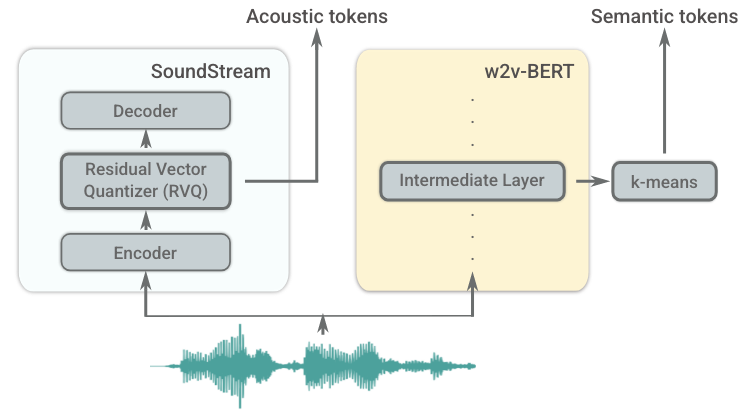
\includegraphics[width=0.5\textwidth]{tokenizerAudioLM.png}
  \caption[AudioLM Tokenisierungsverfahren]{Das hybrides Tokenisierungsverfahren zur Generierung semantischer Tokens mittels \emph{w2v-BERT} \cite{chung_w2v-bert_2021} und akustischer Tokens über \emph{SoundStream} \cite{zeghidour_soundstream_2021} \cite{borsos_audiolm_2022}
}
  \label{fig:tokenizerAudioLM}
\end{subfigure}

\vspace{1em} % Optional: Add some vertical space between the subfigures

\begin{subfigure}{1.0\textwidth}
  \centering
  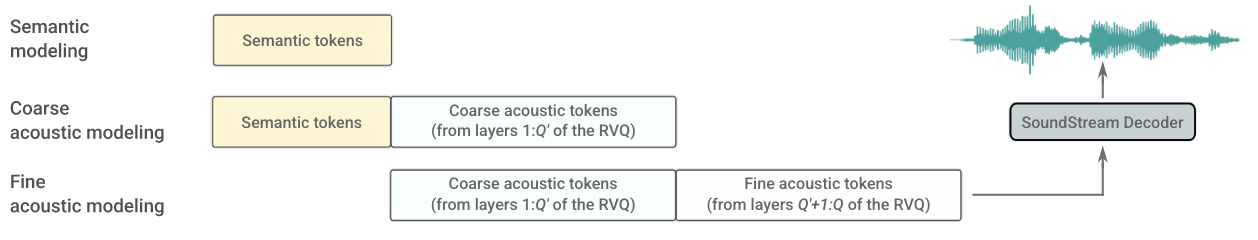
\includegraphics[width=0.7\textwidth]{hierarAudioLM.png}
  \caption[AudioLM Hierarchische Modellierung der Tokens]{Hierarchische Drei-Stufen-Modellierung von Tokens: Zunächst werden semantische Tokens für eine kohärente Struktur generiert. Diese werden anschließend durch grobe akustische Tokens ergänzt. Schließlich werden feine akustische Details in Tokens umgewandelt. Die abschließende Tokensequenz wird mittels \emph{Decoder} in ein Audiosignal transformiert. \cite{borsos_audiolm_2022}}
  \label{fig:hierarAudioLM}
\end{subfigure}
\caption[AudioLM Architektur]{AudioLM Module zur Extraktion von Tokens und Konstruktion eines Klanges aus diesen. \cite{borsos_audiolm_2022}}
\label{fig:test}
\end{figure}

Das Modell \emph{Diffsound} \cite{yang_diffsound_2023} wurde mit der Absicht entwickelt, Soundeffekte zu generieren. Die Erzeugung eines Audiosignals erfolgt anhand eines \emph{Prompts}, unter Zuhilfenahme eines \emph{Text Encoders}, eines \emph{Vector Quantized Variational Autoencoders (\emph{VQ-VAE})}, eines \emph{Token Decoders} und eines \emph{Vocoders} (siehe Abbildung \ref{fig:DiffsoundArchitecture}). Der \emph{Text Encoder} extrahiert relevante Audioinformationen aus dem eingegebenen Text und eliminiert dabei unwesentliche Daten. Dabei kommen ein vorab trainiertes \emph{BERT} \cite{devlin_bert_2019} und der \emph{Text Encoder} eines bereits trainierten \emph{Contrastive Language-Image Pre-Training (CLIP)} \cite{radford_learning_2021} zum Einsatz. Aus diesen Token wird ein \emph{Mel}-Spektrogramm generiert, welches das künftige Audiosignal repräsentiert. Da \emph{Mel}-Spektrogramme in eine Token-Sequenz überführt werden können, erstellt der \emph{Token Decoder} diese basierend auf den vom \emph{Text Encoder} generierten Token. Die Qualität des resultierenden Audiosignals hängt maßgeblich vom \emph{Token Decoder} ab. Frühere Arbeiten \cite{liu_conditional_2021, iashin_taming_2021} setzten auf einen \emph{autoregressiven} Ansatz, welcher aufeinanderfolgende Token basierend auf ihren Vorgängern vorhersagte. Ein solcher Ansatz kann allerdings zu kumulierten Fehlern führen, die sowohl die Rechenzeit als auch die Qualität beeinträchtigen. Zur Überwindung dieser Schwäche präsentiert das Paper einen \emph{nicht autoregressiven Token Decoder}, der auf \emph{Diskreter Diffusion} \cite{sohl-dickstein_deep_2015, austin_structured_2023} basiert. Anstatt die Mel-Spektrogramm-Token sequenziell vorherzusagen, prognostiziert \emph{Diffsound} alle Token simultan und optimiert sie iterativ. Der \emph{VQ-VAE} \cite{oord_neural_2018} lernt mithilfe eines \emph{Discriminators} das Vokabular der Spektrogramm-Token, um ein Spektrogramm zu generieren (siehe Abbildung \ref{fig:VQVAE}). In einem abschließenden Schritt konvertiert der \emph{Vocoder} das erstellte Spektrogramm in ein Audiosignal. Hierzu wurde der \emph{Vocoder MelGAN} \cite{kumar_melgan_2019} mit dem \emph{AudioSet} \cite{gemmeke_audio_2017} Datensatz trainiert. Zusätzlich kam der Datensatz \emph{AudioCaps} \cite{kim_audiocaps_2019} sowohl für Training als auch Validierung zum Einsatz. Trotz der Fortschritte besitzt diese Arbeit Limitierungen: So ist das Generierungssystem nicht vollständig End-to-End und sowohl der \emph{VQ-VAE}, der Token-\emph{Decoder} als auch der \emph{Vocoder} werden separat trainiert. \cite{yang_diffsound_2023}

\begin{figure}[h]
\centering
\begin{subfigure}{1.0\textwidth}
  \centering
  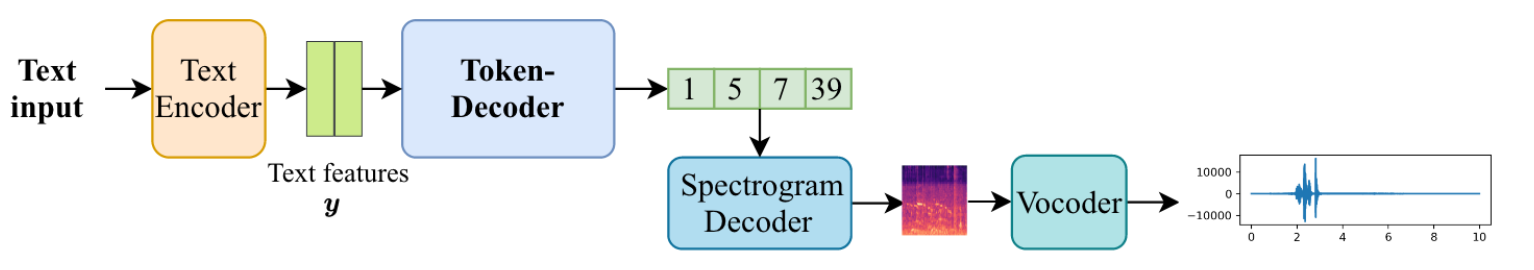
\includegraphics[width=1\textwidth]{Diffsound1.png}
  \caption[Diffsound Architektur]{Umwandlung einer Texteingabe in ein Audiosignal: Mithilfe des \emph{Text Encoder} und des \emph{Token-Decoder} werden Tokens für ein Spektrogramm generiert. Dieses kann anschließend durch einen \emph{Vocoder} in ein Audiosignal transformiert werden. \cite{yang_diffsound_2023}
}
  \label{fig:DiffsoundArchitecture}
\end{subfigure}

\vspace{1em} % Optional: Add some vertical space between the subfigures

\begin{subfigure}{1.0\textwidth}
  \centering
  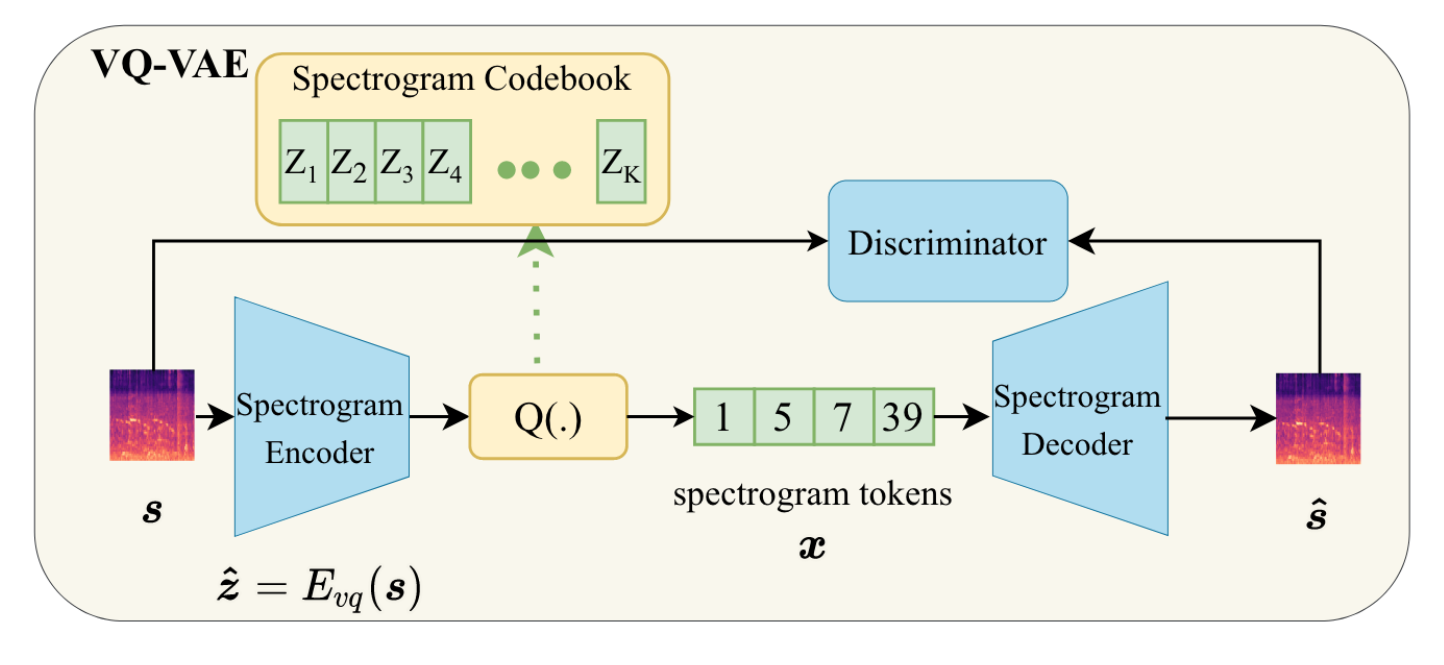
\includegraphics[width=0.7\textwidth]{Diffsound2.png}
  \caption[Diffsound VQ-VAE]{\emph{Diffsound Vector Quantized Variational Autoencoder} für das Erlernen einer latenten Repräsentation von Spektrogrammen: Die Spektrogramme werden kodiert und anschließend rekonstruiert. Die Optimierung erfolgt mithilfe eines \emph{Discriminator}. \cite{yang_diffsound_2023}}
  \label{fig:VQVAE}
\end{subfigure}
\caption[Diffsound Architektur]{Diffsound Architektur: Ablauf der Inferenz und der \emph{Vector Quantized Variational Autoencoder} \cite{yang_diffsound_2023}}
\label{fig:test}
\end{figure}

Einen \emph{autoregressiven} Ansatz verfolgend, verspricht \emph{AudioGen} \cite{kreuk_audiogen_2023} eine verbesserte Audiogenerierung auf der Grundlage textueller Eingaben im Vergleich zu \emph{Diffsound}. \emph{AudioGen} operiert auf einer gelernten diskreten Audio-Repräsentation und ist in der Lage daraus Audiosignale zu generieren. Die Architektur dieses Modells besteht aus zwei Hauptkomponenten (siehe Abbildung \ref{fig:audiogen}). Die erste Komponente kodiert Audio mittels \emph{neural audio compression} \cite{zeghidour_soundstream_2021} in eine diskrete Tokensequenz. Das hierfür verwendete Modell wurde darauf trainiert, komprimierte Audiosignale zu rekonstruieren. Auf die durch diese erste Komponente erzeugten Audio-Tokens versucht ein \emph{autoregressiven} \emph{Transformer-decoder} \emph{Sprachmodell}, das dem \emph{GPT2} \cite{alec_radford_jeff_wu_rewon_child_david_luan_dario_amodei_ilya_sutskever_language_2019} ähnelt, unter Berücksichtigung von Textinformationen abzubilden. Während der Inferenz extrahiert das \emph{Transformer}-Modell die zur Eingabe passenden Tokens, die anschließend durch den \emph{Decoder} der ersten Komponente in Audio umgewandelt werden können. Das entwickelte Modell zeigt jedoch Schwierigkeiten, temporale Umformulierungen korrekt zu verarbeiten. \cite{kreuk_audiogen_2023}

\begin{figure}[h]
  \centering
  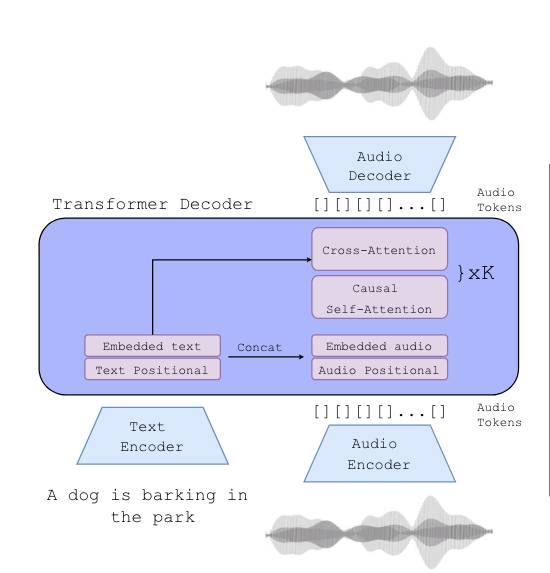
\includegraphics[width=.5\textwidth]{graphics/Audiogen.png}
  \caption[AudioGen Architektur]{Architektur von \emph{AudioGen}: Zusammensetzung aus \emph{Encoder} und \emph{Decoder} zum Erlernen des latenten Raums sowie dem \emph{Transformer}-Modell, das auf diesen operiert. \cite{kreuk_audiogen_2023}}
  \label{fig:audiogen}
\end{figure}

Das Modell \emph{Tango} \cite{ghosal_text--audio_2023} zieht Inspiration aus \emph{AudioLDM} und verfolgt das Ziel, Text in Audio mittels \emph{latenter Diffusion} zu transformieren. Es hebt sich in bestimmten Aspekten von \emph{AudioLDM} ab und strebt an, überlegene Resultate trotz reduziertem Datensatz zu erziehlen. Die Konstruktionsweise setzt sich aus drei zentralen Bestandteilen zusammen (siehe Abbildung \ref{fig:tango}): einem \emph{Text Encoder} zur Verarbeitung der Eingabe-\emph{Prompts}, einem \emph{Latenten Diffusionsmodell} (\emph{LDM}) \cite{rombach_high-resolution_2022}, und einem \emph{Variational Autoencoder} (\emph{VAE}) \cite{kingma_auto-encoding_2022}. Der \emph{Text Encoder}, angereichert durch das \emph{Large Language Model} (\emph{LLM}) \emph{FLAN-T5-LARGE} \cite{chung_scaling_2022}, formt eine textbasierte Darstellung des gegebenen Inputs. Untersuchungen \cite{dai_why_2023} zufolge vermögen \emph{FLAN-T5-Modelle} durch ihr extensives Vortraining - reich an Gedankenstrukturen, Argumentationslinien und Anweisungen - rasch und wirkungsvoll neue Aufgaben zu erlernen. Dieses intensive Vortraining, das älteren Textmodellen wie \emph{RoBERTa} \cite{liu_roberta_2019} fehlte, könnte die Betonung essenzieller Details vereinfachen, was eine optimierte Transformation von Texten in ihre auditiven Pendants begünstigen könnte. Das \emph{LDM}, adaptiert von \emph{AudioLDM}, wandelt die textbasierte Darstellung des \emph{Prompts} in eine latente Audio-Abbildung mittels Spektogramm-Tokens um. Dieser Vorgang beruht auf dem synchronisierten Wechselspiel von Vorwärts- und Rückwärts-\emph{diffusion}: Dem Audio wird Rauschen beigemischt, welches anschließend unter Anleitung des Textes wieder entfernt wird. Bei der Auswertung wird der trainierte Rückwärts \emph{Diffusions}-prozess genutzt, um die Audio-Darstellung zu formen. Der \emph{VAE}-Decoder wandelt dies dann in ein Mel-Spektogramm um. Der \emph{Vocoder HiFi-GAN} \cite{kong_hifi-gan_2020}, identisch zu dem in \emph{AudioLDM}, konvertiert das Spektogramm letztlich in ein Audiosignal. Eine Schwäche des Modells liegt in der Erstellung nuancierter Audio-Outputs für ähnliche Texte, besonders wenn es nur auf kleineren Datensätzen trainiert wurde. Die Autoren empfehlen daher, dieses Hindernis durch Training auf umfangreicheren Datensätzen zu überbrücken, um die Kapazitäten des Modells in Bezug auf Differenzierung und Generierung von diversen Text-Audio-Kombinationen zu steigern. \cite{ghosal_text--audio_2023}

\begin{figure}[h]
  \centering
  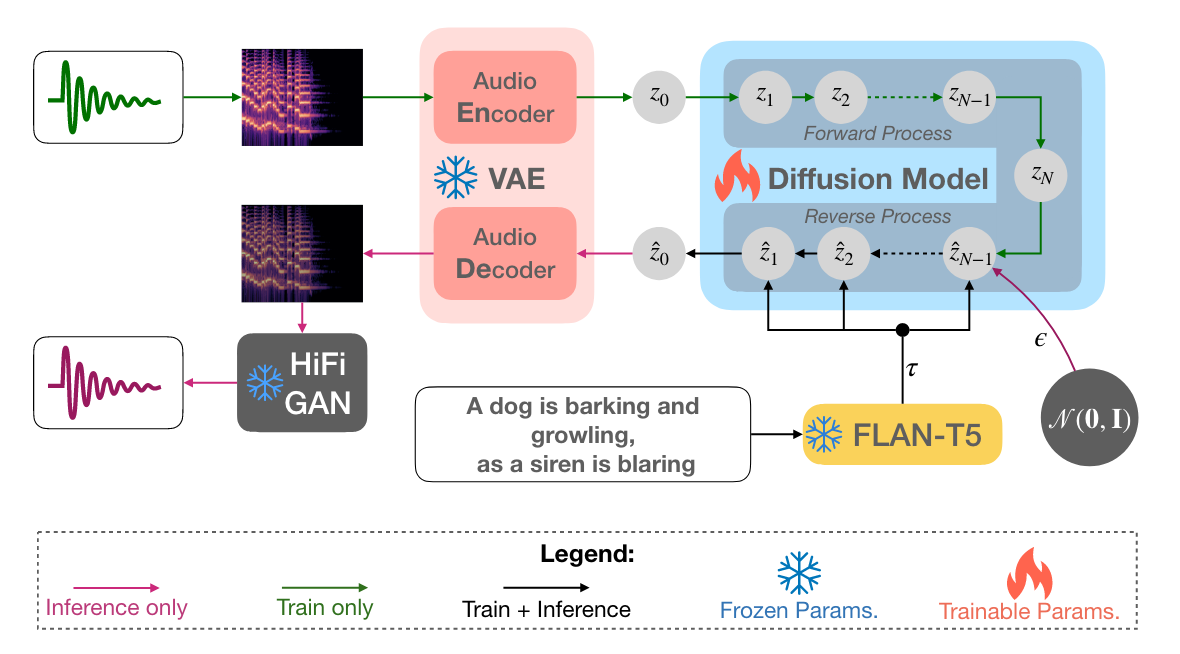
\includegraphics[width=.7\textwidth]{graphics/Tango.png}
  \caption[Tango Architektur]{Architektur von Tango: Ein Spektogramm-\emph{Encoder} und \emph{Decoder} zur Erstellung einer latenten Repräsentation, ergänzt durch den \emph{Diffusions}-Prozess und den Text-\emph{Encoder}. \cite{liu_roberta_2019}}
  \label{fig:tango}
\end{figure}

Ein zusätzliches Modell, das sich der Methode der \emph{Latenten Diffusion} \cite{rombach_high-resolution_2022} bedient, um Text in Audio zu konvertieren, ist \emph{Make-An-Audio} \cite{huang_make--audio_2023}. Parallel zur Entwicklung dieses Modells (siehe Abbildung \ref{fig:Make-An-Audio_Architecture}) wurde eine Methode konzipiert, um ungelabelten Audiosignalen eine Beschreibung zuzuweisen (siehe Abbildung \ref{fig:Make-An-Audio_DestillATIon}). Diese Methode soll den Mangel an gelabelten Audiosignalen adressieren. Der Prozess zur Umschreibung ungelabelter Audiosignale gliedert sich in zwei Stufen. In der ersten Stufe kommen vortrainierte Expertenmodelle \cite{xu_crnn-gru_2020, deshmukh_audio_2022, koepke_audio_2023} zum Einsatz, um Wissen zu destillieren. Diese Modelle generieren Texte, die das Audiosignal beschreiben. Der Text mit der höchsten \emph{CLAP}-Bewertung \cite{elizalde_clap_2022} wird als finaler Text ausgewählt. Zur Vermeidung von Overfitting im Modell wird in der zweiten Stufe aus einer Datenbank mit gelabelten Audioereignissen bis zu zwei Signale extrahiert und mit dem aus dem ersten Schritt generierten Paar kombiniert. Der \emph{Diffusions}-Prozess arbeitet auf einer latenten Repräsentation des Audios, die durch einen Spektrogramm-\emph{Autoencoder} erlernt wurde. Ein \emph{Encoder}-Netz empfängt ein Spektrogramm und komprimiert dieses in den \emph{Latentenraum}. Ein \emph{Decoder} zielt darauf ab, das komprimierte Audiosignal aus dem latenten Raum zu rekonstruieren. Das Modell wird daraufhin trainiert, den durch die Rekonstruktion entstandenen Verlust zu minimieren und mit einem zusätzlichen \emph{Diskriminator}, der das Unterscheiden zwischen echten und generierten Audiosignalen erlernt. Ein \emph{Vocoder} kann schließlich das rekonstruierte Spektrogramm in ein Audiosignal umwandeln. Abseits von textbasierten Eingaben können Audiosignale auch aus anderen Quellen, wie Bildern und Videos, generiert werden. \cite{huang_make--audio_2023}
 

\begin{figure}[h]
\centering
\begin{subfigure}{1.0\textwidth}
  \centering
  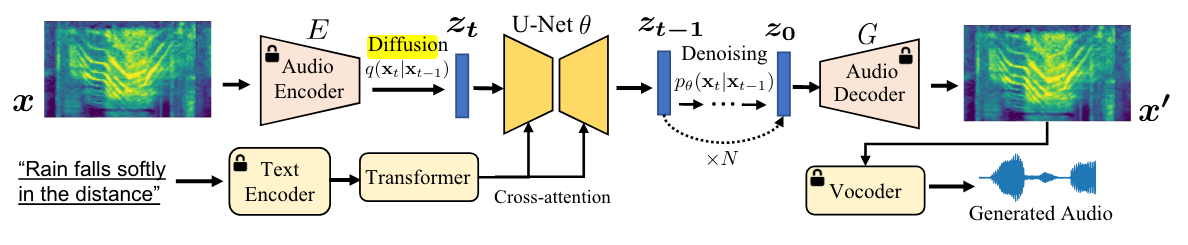
\includegraphics[width=1\textwidth]{graphics/Make-An_Audio.png}
  \caption[Make-An-Audio Architektur]{Architektur von Make-An-Audio: Während des Trainings bleiben die Parameter der mit einem Schloss gekennzeichneten Module, darunter Text-\emph{Encoder}, Audio-\emph{Encoder}, \emph{Decoder} und \emph{Vocoder}, konstant. \emph{U-Net} und der \emph{Diffusions}-Prozess werden trainiert. \cite{huang_make--audio_2023}}
  \label{fig:Make-An-Audio_Architecture}
\end{subfigure}

\vspace{1em} % Optional: Add some vertical space between the subfigures

\begin{subfigure}{1.0\textwidth}
  \centering
  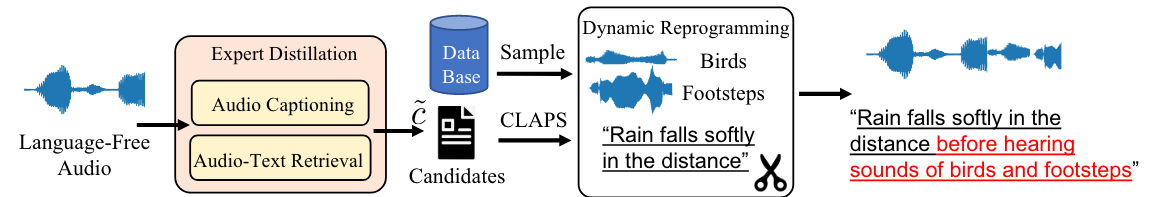
\includegraphics[width=0.7\textwidth]{graphics/Make-An-Audio-Destillation.png}
  \caption[Make-An-Audio Destillation]{Destillation von Make-An-Audio zur Erweiterung des verfügbaren Trainingsdatensatzes \cite{huang_make--audio_2023}}
  \label{fig:Make-An-Audio_DestillATIon}
\end{subfigure}
\caption[Make-An-Audio Module]{Module von Make-An-Audio zur Audio-Synthese und Erweiterung des Datensatzes umschriebener Audioereignisse. \cite{huang_make--audio_2023}}
\label{fig:test}
\end{figure}

Die musikalische Anwendung neuronaler Netze beschränkt sich nicht ausschließlich auf die konditionierte Synthese von Klängen. Vielmehr ermöglichen solche Netzwerke auch eine zielgerichtete musikalische Generierung. Modelle wie \emph{MusicLM} \cite{agostinelli_musiclm_2023} und \emph{MusicGen} \cite{copet_simple_2023} stützen sich auf bewährte Modelle und Ansätze der akustischen Klangsynthese. Sie erweitern diese jedoch durch die Fähigkeit, vollständige musikalische Audiosignale zu generieren, die kohärente Strukturen über längere Zeiträume beibehalten. 

Das Modell \emph{MusicLM} \cite{agostinelli_musiclm_2023} basiert auf den Konzepten von \emph{AudioLM}. Es integriert akustische Informationen über \emph{Soundstream} \cite{zeghidour_soundstream_2021}, semantische Informationen mittels \emph{w2v-Bert} \cite{chung_w2v-bert_2021-1} und Audio-Informationen mithilfe von \emph{Mulan} \cite{huang_mulan_2022} (siehe Abbildung \ref{fig:MusicLM_tokens}). Im Training dieses Modells erfolgte eine Abbildung des latenten Raums von \emph{MuLan} zum latenten Raum von \emph{w2v-Bert} und ebenso eine Abbildung von \emph{w2v-Bert} zu \emph{Soundstream} unter Verwendung von \emph{Transformers}. Während der Inferenz können die erlernten Abbildungen genutzt werden. Eine von \emph{MuLan} generierte Texteingabe wird hierbei in den latenten Raum von \emph{SoundStream} transformiert, um anschließend in ein Audiosignal kodiert zu werden (siehe Abbildung \ref{fig:MusicLM_Inference}). \cite{agostinelli_musiclm_2023}

\begin{figure}[h]
\centering
\begin{subfigure}{.8\textwidth}
  \centering
  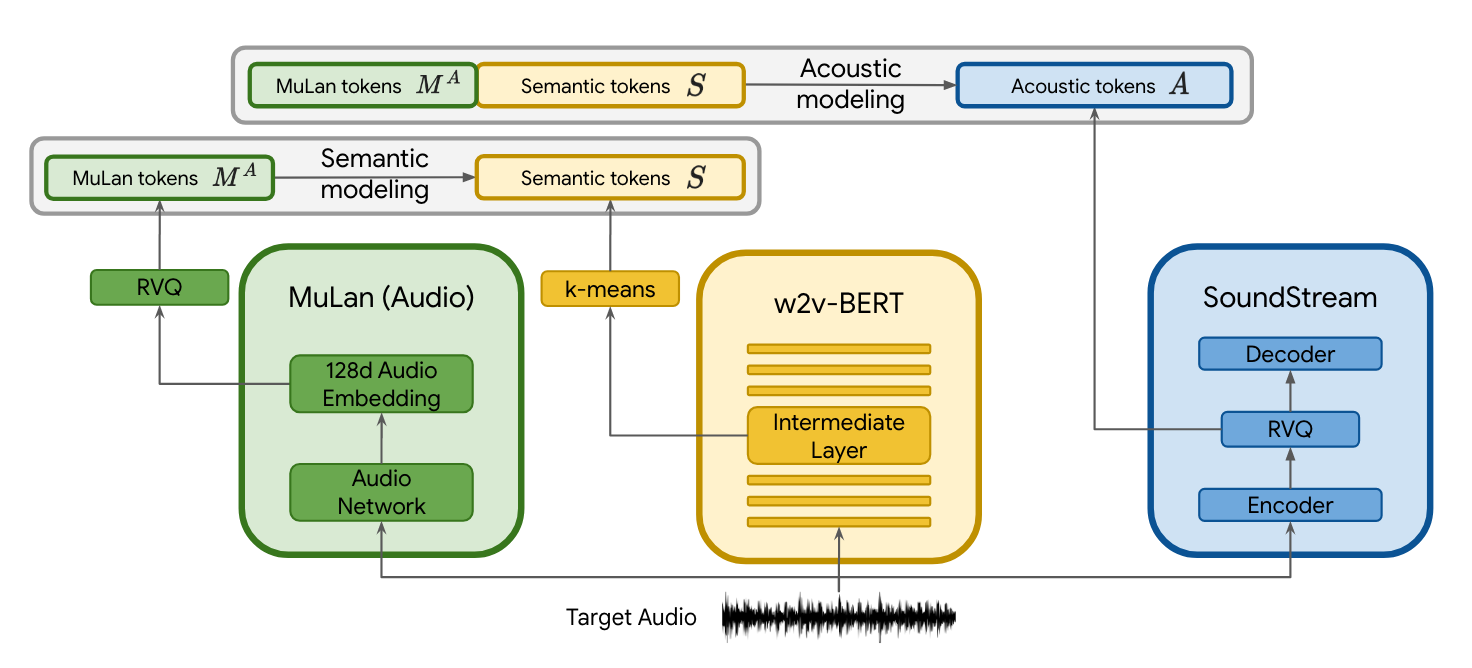
\includegraphics[width=1\textwidth]{graphics/MusicLM1.png}
  \caption[MusicLM Tokenisierung]{Modellierung semantischer und akustischer Tokens erzeugt durch \emph{MuLan}, \emph{w2v-Bert} und \emph{SoundStream}. \cite{agostinelli_musiclm_2023}}
  \label{fig:MusicLM_tokens}
\end{subfigure}

\vspace{1em} % Optional: Add some vertical space between the subfigures

\begin{subfigure}{1.0\textwidth}
  \centering
  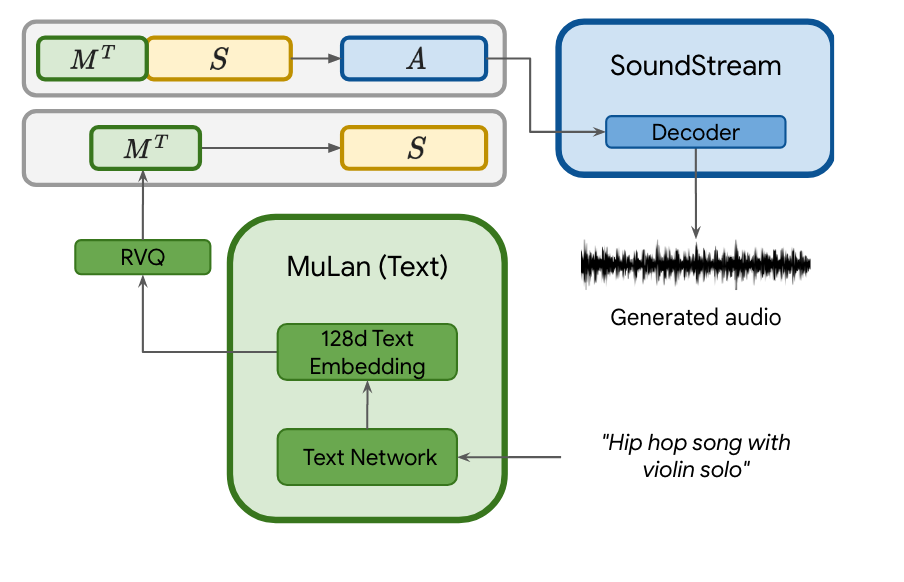
\includegraphics[width=0.5\textwidth]{graphics/MusicLM2.png}
  \caption[MusicLM Inferenz]{Inferenz von MusicLM für Text-zu-Audio-Konversion mittels des Text-\emph{Encoders} \emph{MuLan} und der im Training erlernten Modellierungsverfahren. \cite{agostinelli_musiclm_2023}}
  \label{fig:MusicLM_Inference}
\end{subfigure}
\caption[MusicLM Module]{Module von MusicLM für Inferenzprozesse und Training. \cite{agostinelli_musiclm_2023}}
\label{fig:test}
\end{figure}

Im Gegensatz zu \emph{MusicLM} \cite{copet_simple_2023} setzt \emph{MusicGen} nicht auf mehrere kaskadierende Modelle, sondern verwendet einen \emph{autoregressiven Transformer-basierten Decoder} \cite{vaswani_attention_2017}, der auf Text oder Melodien, wie beispielsweise Summen, konditioniert werden kann. Dieses Modell operiert auf einer komprimierten Darstellung von gesampelten Audiosignalen, die durch \emph{EnCodec} \cite{defossez_high_2022} (siehe Abbildung \ref{fig:encodec})generiert wird. \emph{EnCodec} ist ein \emph{convolutional auto-encoder}, der einen \emph{Latentenraum} mithilfe von \emph{Residual Vector Quantization} \cite{zeghidour_soundstream_2021} erstellt. Abhängig von der Anzahl der in dem Quantifizierungsprozess verwendeten \emph{codebooks} werden entsprechend viele Tokens generiert, die speziell angeordnet und anschließend dem \emph{Decoder} von \emph{EnCodec} übergeben werden. Dieser kann unter der gegebenen Konditionierung eine Audiodatei erstellen. Für die Textkonditionierung wurden Modelle wie \emph{T5} \cite{raffel_exploring_2020}, \emph{FLAN-T5} \cite{roberts_scaling_2022} und \emph{CLAP} evaluiert, während für Melodien eine Konditionierung über ein \emph{Chromagramm} erfolgt. \cite{copet_simple_2023}

\begin{figure}[h]
  \centering
  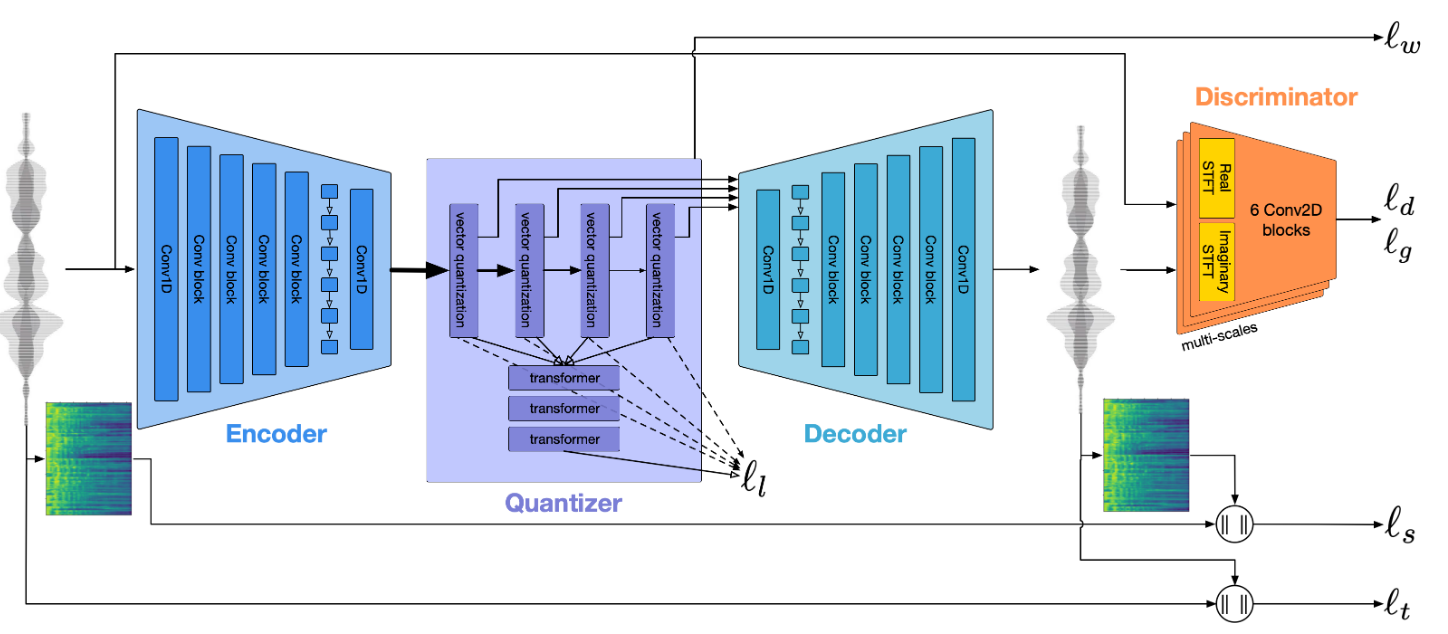
\includegraphics[width=.7\textwidth]{graphics/MusicGen.png}
  \caption[MusicGen EnCodec]{Einsatz von \emph{EnCodec} \cite{defossez_high_2022} in \emph{MusicGen} \cite{copet_simple_2023}: Eine \emph{Encoder}-\emph{Decoder}-Architektur basierend auf dem latenten Raum der \emph{Residual Vector Quantization}, optimiert durch einen \emph{Discriminator}. \cite{defossez_high_2022}}
  \label{fig:encodec}
\end{figure}

In dieser Arbeit wurden die generativen Audiomodelle \emph{AudioLDM} \cite{liu_audioldm_2023} und \emph{AudioLDM2} \cite{liu_audioldm2_2023} für die Auswahl herangezogen. Durch die Integration in das von \emph{Huggingface} \cite{noauthor_hugging_2023} veröffentlichte Python-Paket \emph{Diffusers} \cite{von_platen_diffusers_2023} mittels Anbindung \cite{noauthor_huggingface-audioldm_nodate, noauthor_huggingface-audioldm2_nodate} ist eine effiziente Implementierung dieser Modelle gewährleistet. Die zuvor in \emph{VroomAI} nicht vorhandene Möglichkeit Parameter einzustellen wurde ebenfalls berücksichtigt und implementiert.

\chapter{Grundlagen}

\section{Klangsynthese und Musikproduktion}

\subsection{Mathematische und physikalische Modellierung von Musik und Klang}\label{sec:music_math}
\glqq Musik ist eine Kunstform und kulturelle Aktivität, deren Medium der in Zeit organisierte Klang ist\grqq \footnote{"Music is an art form and cultural activity whose medium is sound organized in time"} \cite{tsuji_physics_2021}. Im Gegensatz zu Rauschen weisen die Klänge, die Musik aufbauen, Strukturen und Zusammenhänge auf, welche für das menschliche Gehör als angenehm wahrgenommen werden \cite{parker_good_2009}. 

Klang charakterisiert sich durch ein intrinsisches Zusammenspiel aus physikalischen und perzeptiven Elementen. Auf der physikalischen Ebene manifestiert sich der Klang als Welle, die durch einen schwingenden Körper erzeugt und von einem Ort zum anderen propagiert. Diese Welle setzt sich aus einem \emph{Grundton} sowie mehreren resonierenden Einzeltönen zusammen. Der resultierende Klang weist eine Vielzahl von \emph{Obertönen} auf, die die charakteristischen klanglichen Eigenschaften, auch \emph{Klangfarben} genannt, hervorbringen. \cite{tsuji_physics_2021, parker_good_2009}

Diese diversen \emph{Töne} sind periodische Schwingungen, definiert durch eine \emph{Tonhöhe/Frequenz} $\omega$ (in $Hz$). Diese kann als Anzahl der Kompressionen an einem festgelegten Punkt pro Sekunde verstanden werden. Der Kehrwert der \emph{Frequenz}, bezeichnet als \emph{Periode} $T=\frac{1}{\omega}$ (in $s$), gibt die Dauer an, die eine Kompression benötigt, um zwei identische Punkte zu durchlaufen. Töne mit einer niedrigen \emph{Frequenz} erscheinen in unserer Wahrnehmung als tief und dumpf, wohingegen Töne mit hohen \emph{Frequenzen} als leicht, schwebend und durchdringend empfunden werden. Die \emph{Amplitude} der Schwingung beschreibt die transportierte Energie und demzufolge die Lautstärke eines Tones. Aufgrund des Abstandsgesetzes wird diese von einer Schallquelle über die logarithmische \emph{Dezibel-Skala} (dB) angegeben. \cite{tsuji_physics_2021, parker_good_2009}

Die Analyse der Struktur eines Klangs konzentriert sich auf die Beziehungen und Interaktionen der diversen Töne, die den Klang konstituieren. Die elementarste Darstellung eines Tones ist der Sinuston, welcher durch eine Sinuskurve repräsentiert wird. Gemäß dem Fourier-Theorem besteht jeder Ton aus einer Kombination verschiedener Sinustöne (siehe Abbildung \ref{fig:evolution}). Dabei wird die tiefste dominierende \emph{Frequenz} als \emph{Grundton} und die höheren \emph{Frequenzen} als \emph{Obertöne} klassifiziert. Diese \emph{Obertöne} variieren in ihrer \emph{Frequenz, Amplitude} sowie ihrem zeitlichen Auf- und Abbau. Ein Oberton, dessen \emph{Frequenz} ein ganzzahliges Vielfaches des \emph{Grundtones} darstellt, wird als \emph{harmonischer} Oberton definiert. Ist dies nicht der Fall, wird der Oberton als \emph{inharmonisch} bezeichnet. Daraus folgt, dass verschiedene Instrumente, obwohl sie denselben Ton erzeugen, identische Grundschwingungen, aber unterschiedliche harmonische und inharmonische \emph{Obertöne} aufweisen. \cite{parker_good_2009, white_physics_2014, ruschkowski_elektronische_2019}

\begin{figure}
  \centering
  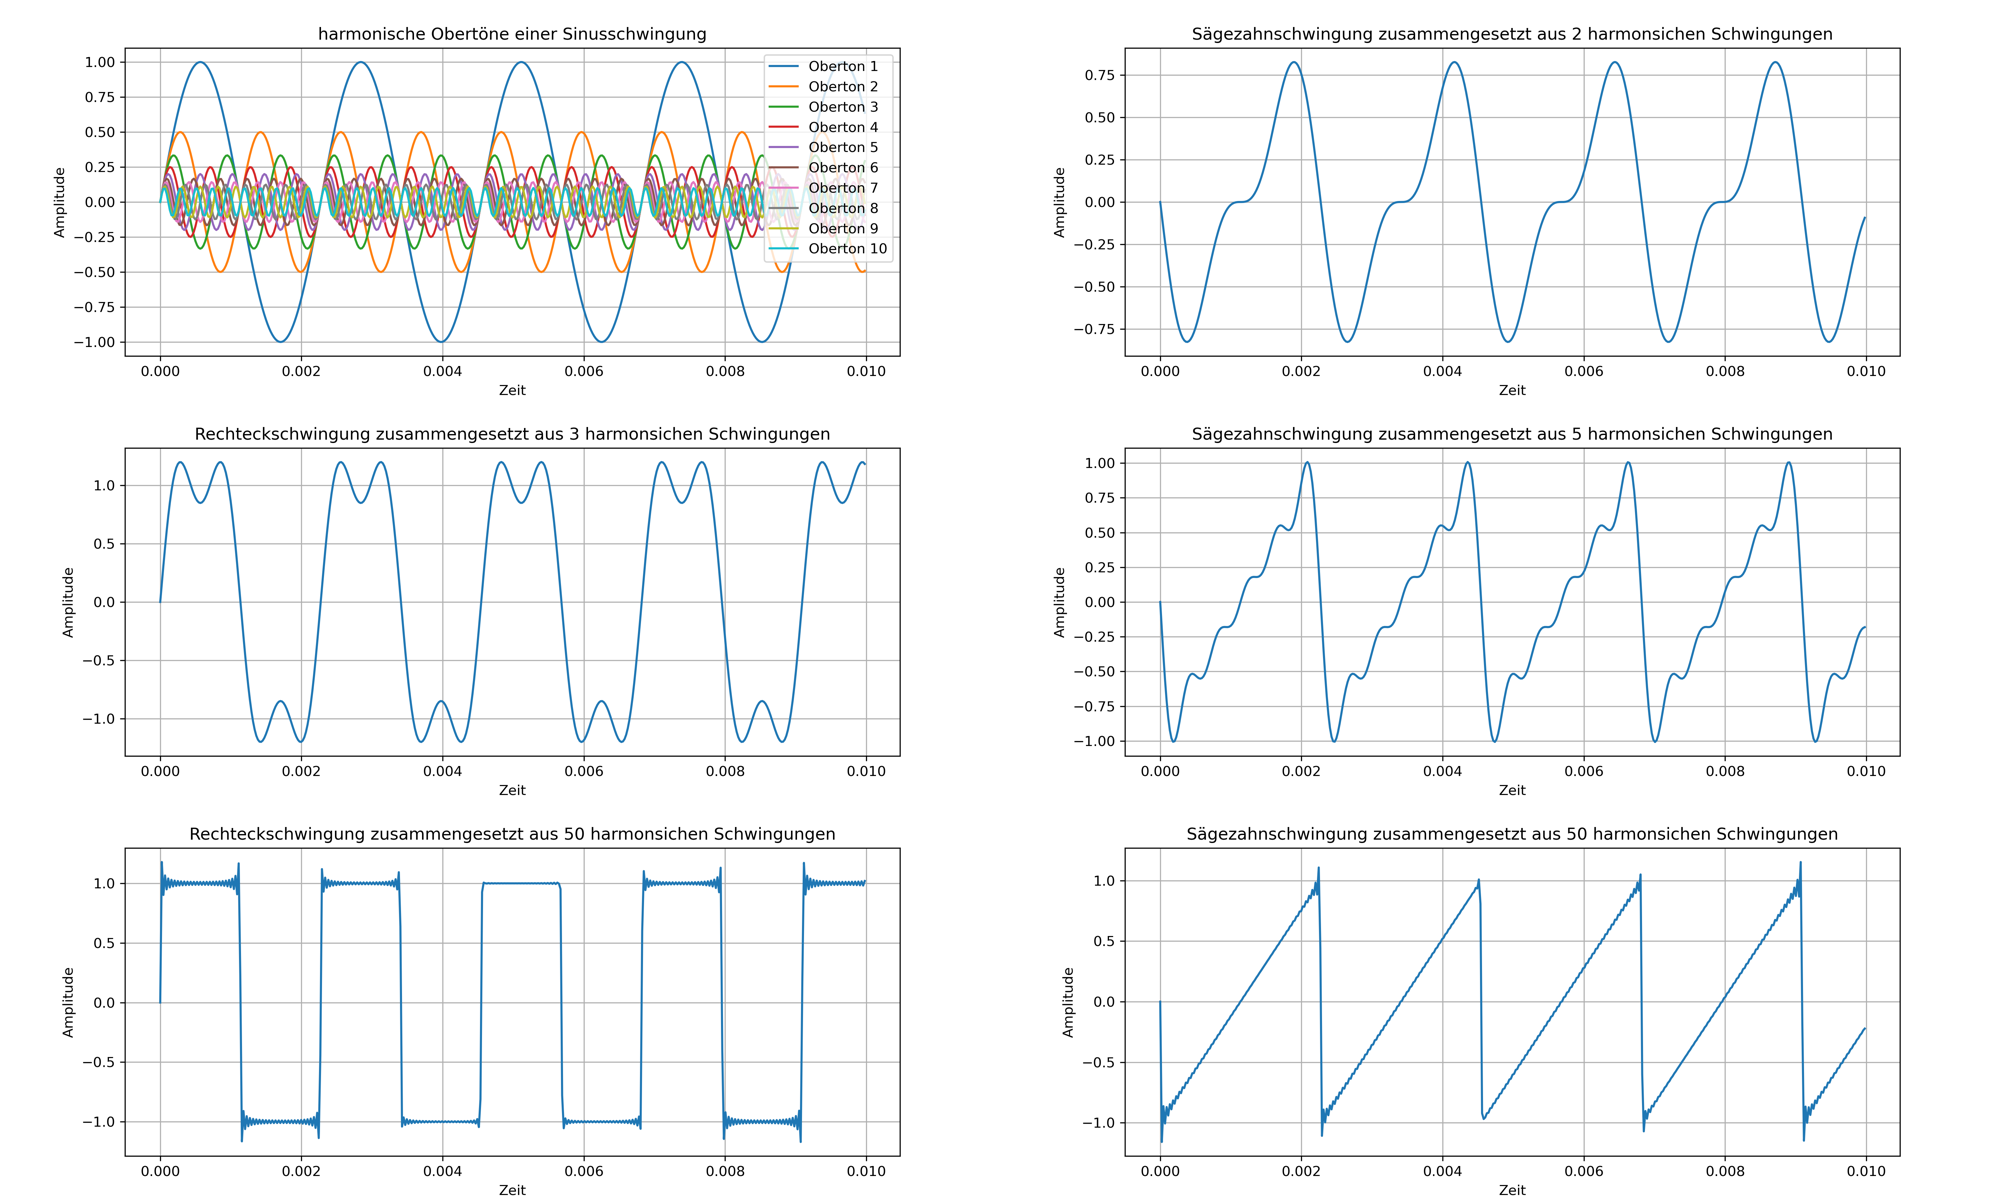
\includegraphics[width=1.0\textwidth]{evolution.png}
  \caption[Fourier Reihe]{Zusammensetzung von Sägezahn- und Rechteckschwingungen aus harmonischen Oberschwingungen einer Sinuswelle.}
  \label{fig:evolution}
\end{figure}

Die Beschaffenheit eines Klangs lässt sich durch die \emph{Amplituden}-faktoren und die korrespondierenden \emph{Frequenzen} der jeweiligen Töne beschreiben und in einem \emph{Frequenzspektrum} (siehe Abbildung \ref{fig:spectro}) darstellen. Diese Visualisierung ermöglicht die Identifikation dominanter \emph{Frequenzen} oder \emph{Frequenz}-bereiche innerhalb des Signals und bietet eine Illustration der \emph{Klangfarbe} sowie der spezifischen Charakteristik des Klangs. Mittels einer \emph{Fourier-Transformation} kann das zugehörige Spektrum für jedes gegebene Signal ermittelt werden. Umgekehrt erlaubt die \emph{Inverse Fourier-Transformation} die Rekonstruktion des Signals basierend auf seinem Spektrum. \cite{raffaseder_audiodesign_2010}

Zur Berechnung einer \emph{Diskreten Fourier-Transformation (DFT)} hat sich die \emph{Fast Fourier-Transformation (FFT)} als effizienter Algorithmus etabliert \cite{heideman_gauss_1985}. Zur Realisierung der Fourier-Transformation in Echtzeit wird auf die \emph{Short Time Fourier-Transformation} zurückgegriffen \cite{thyagarajan_introduction_2019}. 

Ein \emph{Spektrogramm} erlaubt die Analyse eines Signals sowohl im zeitlichen als auch im \emph{Frequenz}-bereich (siehe Abbildung \ref{fig:spectro}). Jedoch ist die Genauigkeit nicht stets gleichbleibend. Bei der Zerlegung des Signals in kurze zeitliche Segmente zur Spektrumsberechnung zeigen längere Segmente eine reduzierte zeitliche Auflösung, profitieren jedoch von einer präziseren Frequenzauflösung. Im Gegensatz dazu bieten kürzere Segmente eine höhere zeitliche Präzision, weisen aber eine geringere Frequenzauflösung auf. \cite{raffaseder_audiodesign_2010}

\emph{Spektogramme}, die sich auf die \emph{Mel-Skala} stützen, nennt man \emph{Mel}-Spektogramm. Diese Skala stellt akustische \emph{Frequenzen} in einer annähernd logarithmischen Weise dar, sodass Tonhöhenintervalle, die ähnlich wahrgenommen werden, über den gesamten Hörbereich konstant abgebildet werden \cite{noauthor_librosamel_frequencies_nodate}.

Ein Klang, der ein kontinuierliches \emph{Frequenzspektrum} (siehe Abbildung \ref{fig:spectro}) aufweist und viele Arten von Geräuschen aus unterschiedlichen Quellen beinhaltet, wird als \emph{Rauschen} definiert \cite{tsuji_physics_2021}.

Der für das menschliche Gehör wahrnehmbare \emph{Frequenz}-bereich, welcher von $20\text{Hz}$ bis $20\text{kHz}$ reicht, lässt sich in drei Segmente unterteilen: \emph{Bässe, Mitten und Höhen}. Die Bässe erstrecken sich von $20\text{Hz}$ bis $250text{Hz}$. Die tiefen Mitten umfassen den Bereich von $250\text{Hz}$ bis $2\text{kHz}$, während sich die hohen Mitten von $2\text{kHz}$ bis $4\text{kHz}$ erstrecken. \emph{Frequenzen} oberhalb von $4\text{kHz}$ werden als Höhen bezeichnet. \cite{raffaseder_audiodesign_2010}

\begin{figure}
  \centering
  \includegraphics[width=1.0\textwidth]{spectrums_flat.png}
  \caption[Spektren, Spektrogramme und Mel-Spektrogramme]{Spektren, Spektrogramme und Mel-Spektrogramme unterschiedlicher Klangcharakteristika.}
  \label{fig:spectro}
\end{figure}


\subsection{Digitale Audiorepräsentation und Sampling}

Aufgrund der binären Beschaffenheit digitaler Computer erfordert die Darstellung und Verarbeitung von Audiosignalen eine Umwandlung des Signals von einem kontinuierlichen in einen diskreten Wertebereich. Das \emph{Abtasttheorem} postuliert, dass analoge Signale redundante Informationen beinhalten, die bei einer Übertragung eliminiert werden können. Daher genügt es, das Audiosignal durch Erfassen von \emph{Amplituden}-werten in regelmäßigen Intervallen zu reproduzieren und zu übermitteln. Um das Signal adäquat zu charakterisieren, sollte die Abtastrate wenigstens das Doppelte der maximalen \emph{Frequenz} des Signals betragen. Diese Schranke wird als \emph{Nyquist-Frequenz} bezeichnet und ist gleich $2 \omega \mathrm{Hz}$. Da das menschliche Ohr lediglich \emph{Frequenzen bis zu $20 \text{kHz}$ detektiert, wird in der Praxis oft eine \emph{Abtastrate} von $44.1\text{kHz}$ angewendet. Unterschreitet die Abtastrate die \emph{Nyquist-Frequenz}, resultiert ein Informationsverlust, und die rekonstruierte Wellenform kann von der ursprünglichen abweichen. In solch einem Szenario ist der Vorgang der Signalrekonstruktion nicht länger deterministisch, was als \emph{Unterabtastung} bezeichnet wird. \cite{lai_practical_2004, shannon_communication_1949, ruschkowski_elektronische_2019}

Die \emph{Samplingtiefe} (engl. \emph{Bitdepth}) definiert den Wertebereich, innerhalb dessen die erfassten \emph{Amplituden}-werte dargestellt werden. Ein größerer Wertebereich ermöglicht eine präzisere Repräsentation des ursprünglichen Signals, erfordert jedoch auch einen erhöhten Speicherbedarf. Ist der Wertebereich hingegen eingeschränkt, müssen die \emph{Amplitudenwerte} intensiver gerundet werden, was zu Artefakten und Unregelmäßigkeiten im Signal führen kann. \cite{thompson_understanding_2005}

\emph{Sound-Sampling} oder schlicht \emph{Sampling} in Verbindung mit digitaler oder analoger Klangmodifikation stellt eine eigenständige Technik der Klangsynthese dar. Obwohl es im Wesentlichen eine Reproduktion des entnommenen Signals darstellt, geht es über eine bloße Speicherung hinaus. Prinzipien und Verfahren aus der analogen Synthese und Klanggestaltung können auf die Reproduktion des Klangs angewendet werden. Das resultierende Instrument wird als \emph{Sampler} bezeichnet. Abhängig von seiner Komplexität ermöglicht es dem Nutzer, das Signal in einem definierten Bereich zu wiederholen, zu verlangsamen, zu beschleunigen, zu invertieren oder spezifische Intervalle neu zu ordnen. Dies bietet auch die Gelegenheit zum musikalischen Zitieren, was jedoch rechtliche Fragen bezüglich des klanglichen Diebstahls für Musiker, Verlage und Plattenlabels aufwirft. \cite{russ_sound_2009, ruschkowski_elektronische_2019, katz_capturing_2010}

Die Wiederverwendung und Aufarbeitung von Teilen oder vollständigen, bereits produzierten Werken ist in der Industrie gängige Praxis. Dieses Vorgehen könnte durch den Einsatz generativer künstlicher Intelligenz vermieden werden.

\subsection{Synthetisierung und Klangformung} \label{sec:synth+envelope}

Instrumente, die dazu dienen, musikalische Klänge durch elektronische Spannung zu generieren und zu manipulieren, werden als \emph{Synthesizer} bezeichnet \cite{dudenredaktion_synthesizer_nodate, pirkle_designing_2021}. Die Bestandteile eines solchen Instruments lassen sich in drei Hauptkategorien einteilen (siehe Abbildung \ref{fig:synth}): \emph{Erzeuger} (engl. \emph{source}), \emph{Modifikatoren} (engl. \emph{modifier}) und \emph{Kontrollinstanzen} (engl. \emph{controls}). Erzeuger, wie beispielsweise Oszillatoren, generieren den Grundklang, welcher in diesem speziellen Projekt durch ein generatives \emph{Diffusions}-Modell erzeugt wird. Modifikatoren, zu denen Filter und Effekte gehören, bearbeiten diesen generierten Klang. Kontrollinstanzen ermöglichen es dem Nutzer, die Parameter der Erzeuger und Modifikatoren zu definieren und flexibel anzupassen. Die Veränderung eines Parameters wird als \emph{Modulieren} bezeichnet, während die spezifischen Einstellungen der Parameter als \emph{Patch} gelten. \cite{pirkle_designing_2021}   

Die für die Realisierung des Projekts erforderlichen Komponenten werden im Nachfolgenden erläutert.

\begin{figure}[h]
  \centering
  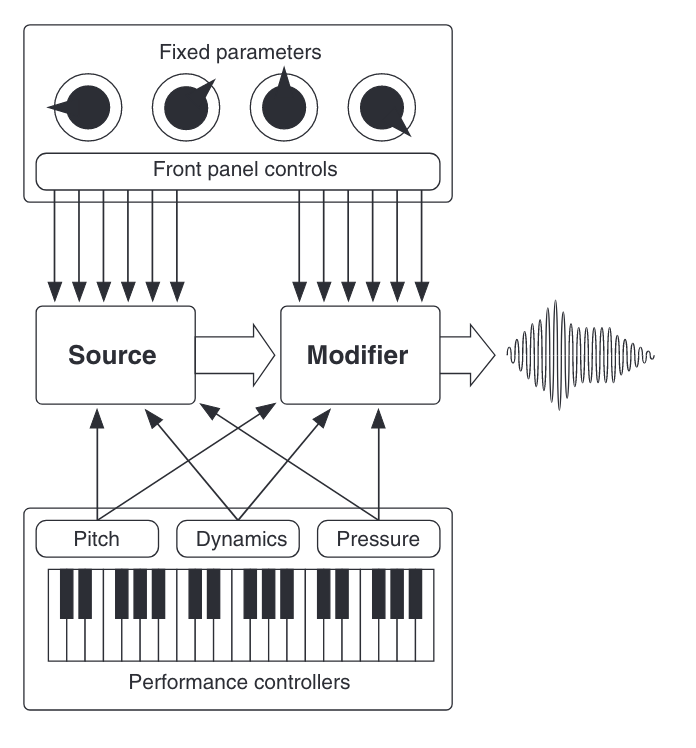
\includegraphics[width=.5\textwidth]{graphics/synthstruc.png}
  \caption[Synth]{Bestandteile eines Synthesizers: \emph{Erzeuger}, \emph{Modifikatoren} und \emph{Kontrollinstanzen}. \cite{russ_sound_2009}}
  \label{fig:synth}
\end{figure}


In dem Bestreben, sein fundiertes wissenschaftliches Verständnis und seine Expertise in den Bau musikalischer Instrumente zu integrieren, konzipierte der Physiker und Komponist Hugh Le Caine erste Apparaturen zur elektronischen Klangsynthese - und das 20 Jahre vor der Kommerzialisierung der ersten analogen Synthesizer \cite{young_gale_hugh_2013}. In diesem Zusammenhang formulierte Le Caine mehrere Grundsätze, die ein Instrumentenentwickler nach seiner Meinung verfolgen sollte. Er war der festen Überzeugung, dass ein Musiker maximale Kontrolle über die zentralen Parameter eines Klangs haben sollte. Dabei identifizierte er, dass die Ausdruckskraft eines Instruments insbesondere durch die Steuerung der \emph{Anschlagsdynamik} über den gesamten Lautstärkebereich eines Tones, durch die Regulierung seiner \emph{An- und Ausschwingszeiten} sowie durch die \emph{Klangfarbe} bestimmt wird. \cite{ruschkowski_elektronische_2019}

\begin{figure}[h]
  \centering
  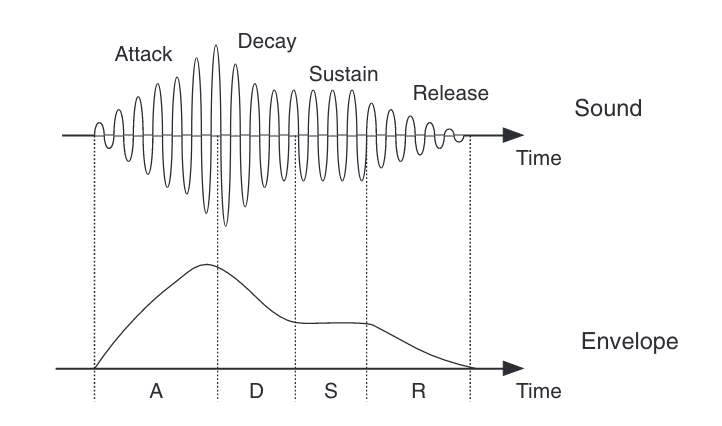
\includegraphics[width=.7\textwidth]{graphics/ADSR.png}
  \caption[Hüllkurve]{Beispiel einer Hüllkurve, definiert durch \emph{Anschwellzeit}, \emph{Abschwellzeit}, \emph{Lautstärkeniveau} und \emph{Ausklingzeit}. \cite{russ_sound_2009}}
  \label{fig:adsr}
\end{figure}

Allgemein wird das Ziel verfolgt, Töne zu generieren, die sich sowohl zeitlich als auch in ihrer \emph{Frequenz} verändern oder übergehen, um akustisch ansprechende Ergebnisse zu erzielen \cite{pirkle_designing_2021}. Die Steuerung von Anschlagsdynamik sowie An- und Ausschwingszeiten wird durch einen \emph{Hüllkurvengenerator} (engl. \emph{envelope generator}) ermöglicht. Dieser Generator besteht in der Regel aus vier Teilen. Die \emph{Anschwellzeit} (engl. \emph{attack time}) gibt die Dauer an, die nach dem Anschlagen einer Taste vergeht, bis ein Ton seine höchste Lautstärke erreicht. Entsprechend bestimmt die \emph{Abschwellzeit} (engl. \emph{decay time}) den Zeitraum, in dem der Ton bis zu einem voreingestellten \emph{Lautstärkeniveau} (engl. \emph{sustain level}) abfällt. Dieses Niveau wird beibehalten, bis die Taste losgelassen wird. Danach kann eine Zeitspanne festgelegt werden, in der der Ton komplett ausklingt (engl. \emph{release time}). Aufgrund der Bezeichnungen dieser Teile wird der Generator oft als \emph{ADSR}-Generator (engl. \emph{attack, decay, sustain, release}) (Abbildung \ref{fig:adsr}) genannt. Instrumente wie Streichinstrumente, die mit einem Bogen gespielt werden, haben lange Anschwell-, Abschwell- und Ausschwingzeiten. Im Gegensatz dazu haben gezupfte Instrumente kürzere Anschwellzeiten. Klaviere und Schlaginstrumente zeichnen sich durch sehr schnelle Anschwellzeiten aus. \cite{ruschkowski_elektronische_2019, russ_sound_2009}

Die \emph{Klangfarbe}, die durch den speziellen Erzeuger entsteht, kann durch Filter weiter verändert werden. In der Elektrotechnik werden diese verwendet, um bestimmte \emph{Frequenzen} zu entfernen. Insbesondere der \emph{Tiefpassfilter} (engl. \emph{low-pass}) und der \emph{Hochpassfilter} (engl. \emph{high-pass}) sind wichtig, da sie entweder die höheren oder tieferen Teile des \emph{Frequenz}-spektrums reduzieren. Der Punkt, an dem diese Reduzierung beginnt, wird als \emph{Beschneidungsfrequenz} (engl. \emph{cut-off-frequency}) bezeichnet. Mit diesen Filtern kann man bestimmte \emph{Obertöne} verstärken oder abschwächen. Wenn man diese Filter hintereinander schaltet, erhält man einen \emph{Bandpassfilter}. Es ist auch möglich, \emph{Obertöne} in der Nähe der Beschneidungsfrequenz zu betonen, was eine \emph{Resonanz} (engl. \emph{resonance}) nachahmt. \cite{ruschkowski_elektronische_2019}

\emph{Kontrollinstanzen} können in zwei Gruppen eingeteilt werden. Die erste Gruppe beinhaltet Steuerelemente, die durch die Performance beeinflusst werden, wie z.B. ein Klaviaturkeyboard. Dies ermöglicht dem Musiker, die Tonhöhe nach seinen Wünschen zu verändern und so das Instrument zu steuern. Die zweite Gruppe umfasst feste Parameter, die spezifisch für den Synthesizer sind. Diese werden verwendet, um die Klangcharakteristik zu bestimmen. Dazu gehören zum Beispiel die Drehregler und Tasten eines Synthesizers. \cite{russ_sound_2009}

Das Kommunikationsprotokoll \emph{MIDI} (\emph{Musical Instrument Digital Interface}) \cite{midi_association_midi_nodate} wurde eingeführt, um eine einheitliche Steuerung von Parametern und Kommunikation zwischen elektronischen Geräten zu gewährleisten. Es hat sich als globaler Standard in der elektronischen Musikbranche etabliert und erlaubt MIDI-Instrumenten, Daten auszutauschen. \cite{ruschkowski_elektronische_2019}

Die Einführung des \emph{MIDI}-Protokoll hatte einen erheblichen Einfluss auf die Entwicklung und das Design von Synthesizern. Aufgrund der durch MIDI bedingten Standardisierung vieler Designaspekte von Synthesizern wurde die Klangerzeugungsmethode prominenter, während das funktionale Instrumentendesign weniger betont wurde. \cite{russ_sound_2009}

\section{Synthetisierung mittels Diffusion}

\glqq Die Methoden der Klangerzeugung mit traditionellen mechanischen Musikinstrumenten waren seit ihrer Entstehung nur unwesentlichen Veränderungen unterworfen. [...] Der Instrumentenbau wandelte sich lediglich deshalb im Laufe der Zeit, weil man die Spielbarkeit der Instrumente zu verbessern und ihren Klangcharakter den wechselnden musikalischen Idealvorstellungen anzupassen wünschte. Anders dagegen im Bereich elektronischer Klangerzeugung. Hier werden ständig neue Methoden zur Synthese von Klängen entwickelt.\grqq \, \cite{ruschkowski_elektronische_2019}

Die innovative Technik der Soundsynthese durch \emph{Diffusion} bietet verschiedene Vorteile. Sie könnte die Abhängigkeit von aufgezeichneten Klängen, deren Aufnahme oft kostenintensiv ist, reduzieren. Künstliche Intelligenz in der Sound-Synthese könnte diesen Sektor demokratisieren und mehr Menschen Zugang zu benötigten Ressourcen bieten. Zudem könnten Nutzer mehr Kontrolle über \emph{Klangfarben} und -eigenschaften erhalten. Kreativ gesehen ermöglicht diese Methode die Schaffung einzigartiger Klänge, die Künstlern als Inspirationsquelle dienen könnten. \cite{haohe_liu_audioldm_2023}


\subsection{Diffusion}
Unter der Prämisse, dass die untersuchten Daten einer bestimmten Verteilung entstammen, zielen generative \emph{Machine-Learning}-Modelle darauf ab, diese Verteilung zu identifizieren und zu approximieren. Die Erstellung neuer Daten erfolgt durch das Ziehen einer Probe aus dieser nachgebildeten Verteilung. \cite{machine_learning_at_berkeley_diffusion_2022}

Der Prozess der \emph{Diffusion} im Maschinellen Lernen \cite{sohl-dickstein_deep_2015, ho_denoising_2020, nichol_improved_2021, dhariwal_diffusion_2021} wurde von der statistischen Thermodynamik \cite{jarzynski_equilibrium_1997} und der sequenziellen Monte-Carlo-Methodik \cite{neal_annealed_1998} inspiriert. Ziel ist es, iterative Verzerrungen einer Datenverteilung $x_0\sim q(\mathbf{x}_0)$ (\emph{forward diffusion}) durch einen umgekehrten Prozess zu korrigieren (\emph{reverse diffusion}). Das Ergebnis ist ein generatives Modell, das effizienter trainiert und bewertet werden kann als vergleichbare Ansätze. \cite{sohl-dickstein_deep_2015, nichol_improved_2021}

\begin{figure}[h]
  \centering
  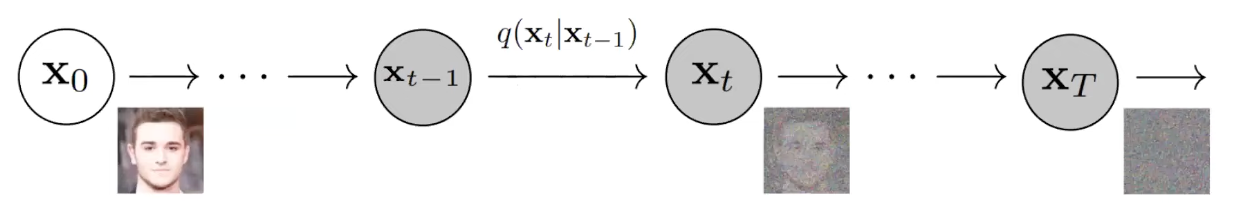
\includegraphics[width=.9\textwidth]{forwardDiffusion.png}
  \caption[Vorwärtsprozess Diffusion]{Vorwärts \emph{Diffusions}-prozess: Schrittweise Korruption betrachteter Daten hin zu isotropischem Rauschen. \cite{machine_learning_at_berkeley_diffusion_2022}}
  \label{fig:forwardDiffusion}
\end{figure} 

Der Vorwärtsprozess (Abbildung \ref{fig:forwardDiffusion}) ist als Markov-Kette gestaltet \cite{sohl-dickstein_deep_2015, ho_denoising_2020}. Einem Datenpunkt $x_0$ wird ein geringes Rauschen hinzugefügt, das durch den Hyperparameter $\left\{\beta_t \in(0,1)\right\}_{t=1}^T$, auch als \emph{noise schedule} bekannt, bestimmt wird \cite{ho_denoising_2020, machine_learning_at_berkeley_diffusion_2022}. Hierbei wird \emph{Gauss'sches Rauschen} \cite{shannon_communication_1949} verwendet, repräsentiert durch eine Normalverteilung $\mathcal{N}$. Wiederholt man diesen Vorgang über $T$ Schritte, werden sukzessive Informationen entfernt, bis schließlich nur isotropisches Rauschen verbleibt \cite{machine_learning_at_berkeley_diffusion_2022}.

\begin{align}
   & q\left(\mathbf{x}^{(t)} \mid \mathbf{x}^{(t-1)}\right) = \mathcal{N}\left(\mathbf{x}^{(t)} ; \mathbf{x}^{(t-1)} \sqrt{1-\beta_t}, \mathbf{I} \beta_t\right) \\
   & q\left(\mathbf{x}_{1: T} \mid \mathbf{x}_0\right)=\prod_{t=1}^T q\left(\mathbf{x}_t \mid \mathbf{x}_{t-1}\right)
\end{align}

Unter Verwendung der Relation \( \alpha_t:=1-\beta_t \) und \( \bar{\alpha}_t:=\prod_{s=1}^t \alpha_s \) lässt sich die Gleichung für den Vorwärtsprozess wie folgt formulieren \cite{ho_denoising_2020}: 

\begin{equation}
    q\left(\mathbf{x}_t \mid \mathbf{x}_0\right)=\mathcal{N}\left(\mathbf{x}_t ; \sqrt{\bar{\alpha}_t} \mathbf{x}_0,\left(1-\bar{\alpha}_t\right) \mathbf{I}\right)
\end{equation}

\begin{figure}[h]
  \centering
  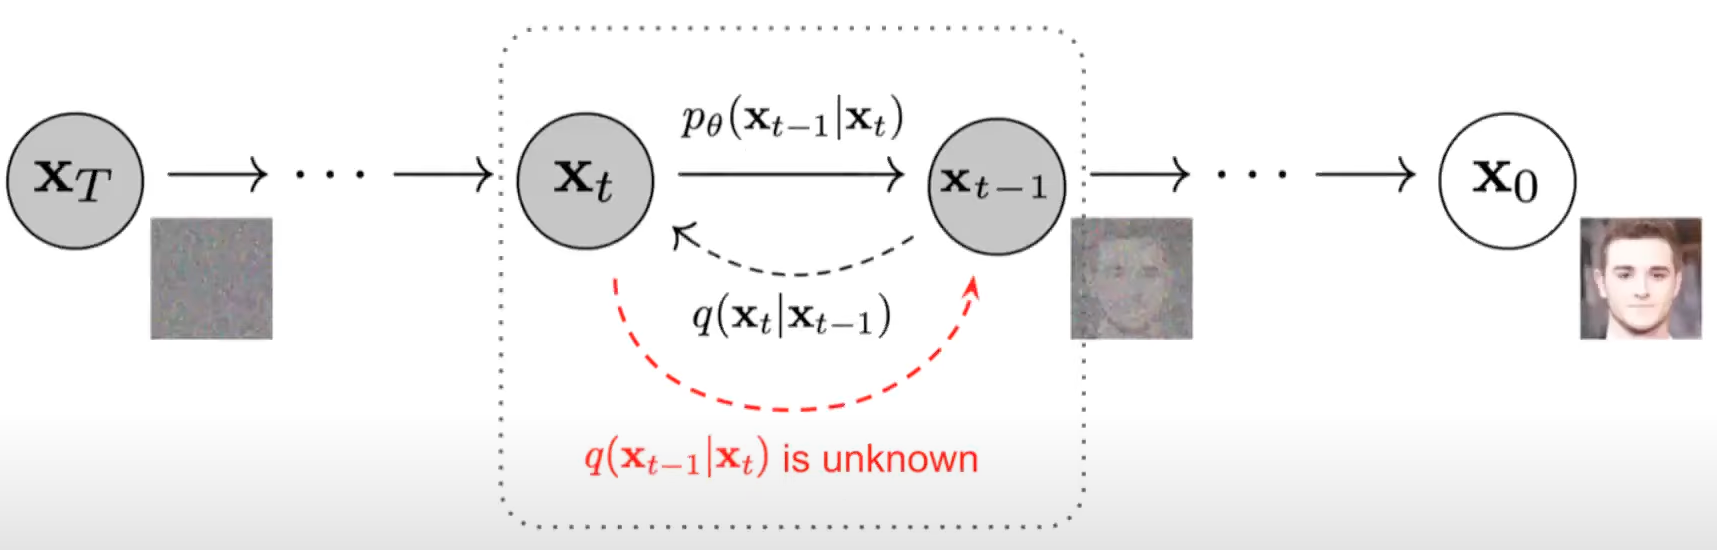
\includegraphics[width=.8\textwidth]{reverseDiffusion.png}
  \caption[Rückwertsprozess Diffusion]{Rückwärts \emph{Diffusions}-prozess: Schrittweise Entrauschung der Daten. \cite{machine_learning_at_berkeley_diffusion_2022}}
  \label{fig:reverseDiffusion}
\end{figure} 

Während des Rückwärtsprozesses (siehe Abbildung \ref{fig:reverseDiffusion}) wird versucht, das eingefügte Rauschen $\epsilon \sim \mathcal{N}(0,1)$ schrittweise zu entfernen \cite{machine_learning_at_berkeley_diffusion_2022}. Dies lässt den umgekehrten Prozess so erscheinen, als würde er aus dem Rauschen neue Daten generieren \cite{machine_learning_at_berkeley_diffusion_2022}. Bei einem niedrigen Wert von $\beta$ stimmt die Rauschverteilung des Rückwärtsschritts \( q\left(\mathbf{x}_{t-1} \mid \mathbf{x}_t\right) \) mit dem Vorwärtsprozess überein \cite{sohl-dickstein_deep_2015}. Der erlernte Rückwärtsprozess \( p_\theta\left(\mathbf{x}_{t-1} \mid \mathbf{x}_t\right) \) kann dementsprechend approximiert werden \cite{ho_denoising_2020, machine_learning_at_berkeley_diffusion_2022, nichol_improved_2021}. Das Training fokussiert sich darauf, kleinere Abweichungen zu schätzen, anstatt den gesamten Ablauf in einem einzigen Schritt durch eine Funktion zu repräsentieren \cite{sohl-dickstein_deep_2015}.


\begin{align}
& p_\theta\left(\mathbf{x}_{t-1} \mid \mathbf{x}_t\right)=\mathcal{N}\left(\mathbf{x}_{t-1} ; \boldsymbol{\mu}_\theta\left(\mathbf{x}_t, t\right), \boldsymbol{\Sigma}_\theta\left(\mathbf{x}_t, t\right)\right)\\
& p_\theta\left(\mathbf{x}_{0: T}\right)=p\left(\mathbf{x}_T\right) \prod_{t=1}^T p_\theta\left(\mathbf{x}_{t-1} \mid \mathbf{x}_t\right)
\end{align}

Das Erlernen des Rückwärtsprozesses wird durch ein neuronales Netzwerk durchgeführt. In jedem Schritt können das Netzwerk den Erwartungswert $\boldsymbol{\mu}_\theta$, das ursprüngliche Bild $\boldsymbol{x}_0$ oder das hinzugefügte Rauschen $\boldsymbol{\epsilon}$ vorhersagen \cite{ho_denoising_2020, nichol_improved_2021}. Untersuchungen zeigten, dass die Vorhersagen des Bildes weniger präzise waren. Daher wurde die Entscheidung getroffen, das hinzugefügte Rauschen $\boldsymbol{\epsilon}$ unter Verwendung der vereinfachten Verlustfunktion 3.6 vorherzusagen \cite{ho_denoising_2020}.

\begin{equation}
    L_{\text {simple }}=E_{t, x_0, \epsilon}\left[\left\|\epsilon-\epsilon_\theta\left(x_t, t\right)\right\|^2\right]
\end{equation}

Der Erwartungswert $\boldsymbol{\mu}_\theta$ kann aus dem vorhergesagten Rauschen $\boldsymbol{\epsilon}$ mithilfe der nachstehenden Gleichung abgeleitet werden \cite{ho_denoising_2020}:

\begin{equation}
    \mu_\theta\left(x_t, t\right)=\frac{1}{\sqrt{\alpha_t}}\left(x_t-\frac{\beta_t}{\sqrt{1-\bar{\alpha}_t}} \epsilon_\theta\left(x_t, t\right)\right)
\end{equation}

Die in \cite{ho_denoising_2020} präsentierte Architektur des neuronalen Netzwerks basiert auf einem \emph{U-Net} \cite{ronneberger_u-net_2015}, welches auf einem \emph{Wide ResNet} \cite{zagoruyko_wide_2017} aufbaut \cite{ho_denoising_2020}.

In \cite{nichol_improved_2021} wurden signifikante Verbesserungen im Vergleich zu den Arbeiten von \cite{sohl-dickstein_deep_2015} und \cite{ho_denoising_2020} vorgenommen. Eine dieser Neuerungen war das Lernen der Varianz anstelle ihrer festen Einstellung. Zudem wurde der \emph{schedule} Parameter optimiert. Statt einer konstanten Einstellung, die dazu führte, dass die Datenpunkte am Ende übermäßig verrauscht waren und die anfänglichen Schritte zu viel Information verloren, wurde ein \emph{cosinus schedule} eingeführt. \cite{nichol_improved_2021}

\subsection{Latente Diffusion}

In \cite{rombach_high-resolution_2022} wurde das \emph{Latente \emph{Diffusions}-modell} (\emph{LDM}) vorgestellt, welches den \emph{Diffusions}-prozess \cite{sohl-dickstein_deep_2015, ho_denoising_2020, nichol_improved_2021, dhariwal_diffusion_2021} erweitert, um die Generierung von Bildern basierend auf einer Eingabe zu ermöglichen. Anders als bei früheren \emph{Diffusions}-prozessen fokussiert sich dieser Ansatz nicht auf die Pixelwerte der Bilder, sondern auf ihre \emph{latente} Darstellung. Dies reduziert den Rechenaufwand erheblich und ermöglicht sowohl das Training als auch die Inferenz auf eingeschränkter Hardware. Die in Abbildung \ref{fig:LDM} dargestellte Architektur besteht aus drei Hauptteilen: Ein \emph{Variational Autoencoder}, der die Daten im \emph{Latentenraum} kodiert und dekodiert, der \emph{Diffusions}-teil und ein zusätzliches Modul, das den \emph{Diffusions}-teil mithilfe von Text, Bildern oder anderen Eingaben konditioniert. \cite{rombach_high-resolution_2022}

\begin{figure}[h]
  \centering
  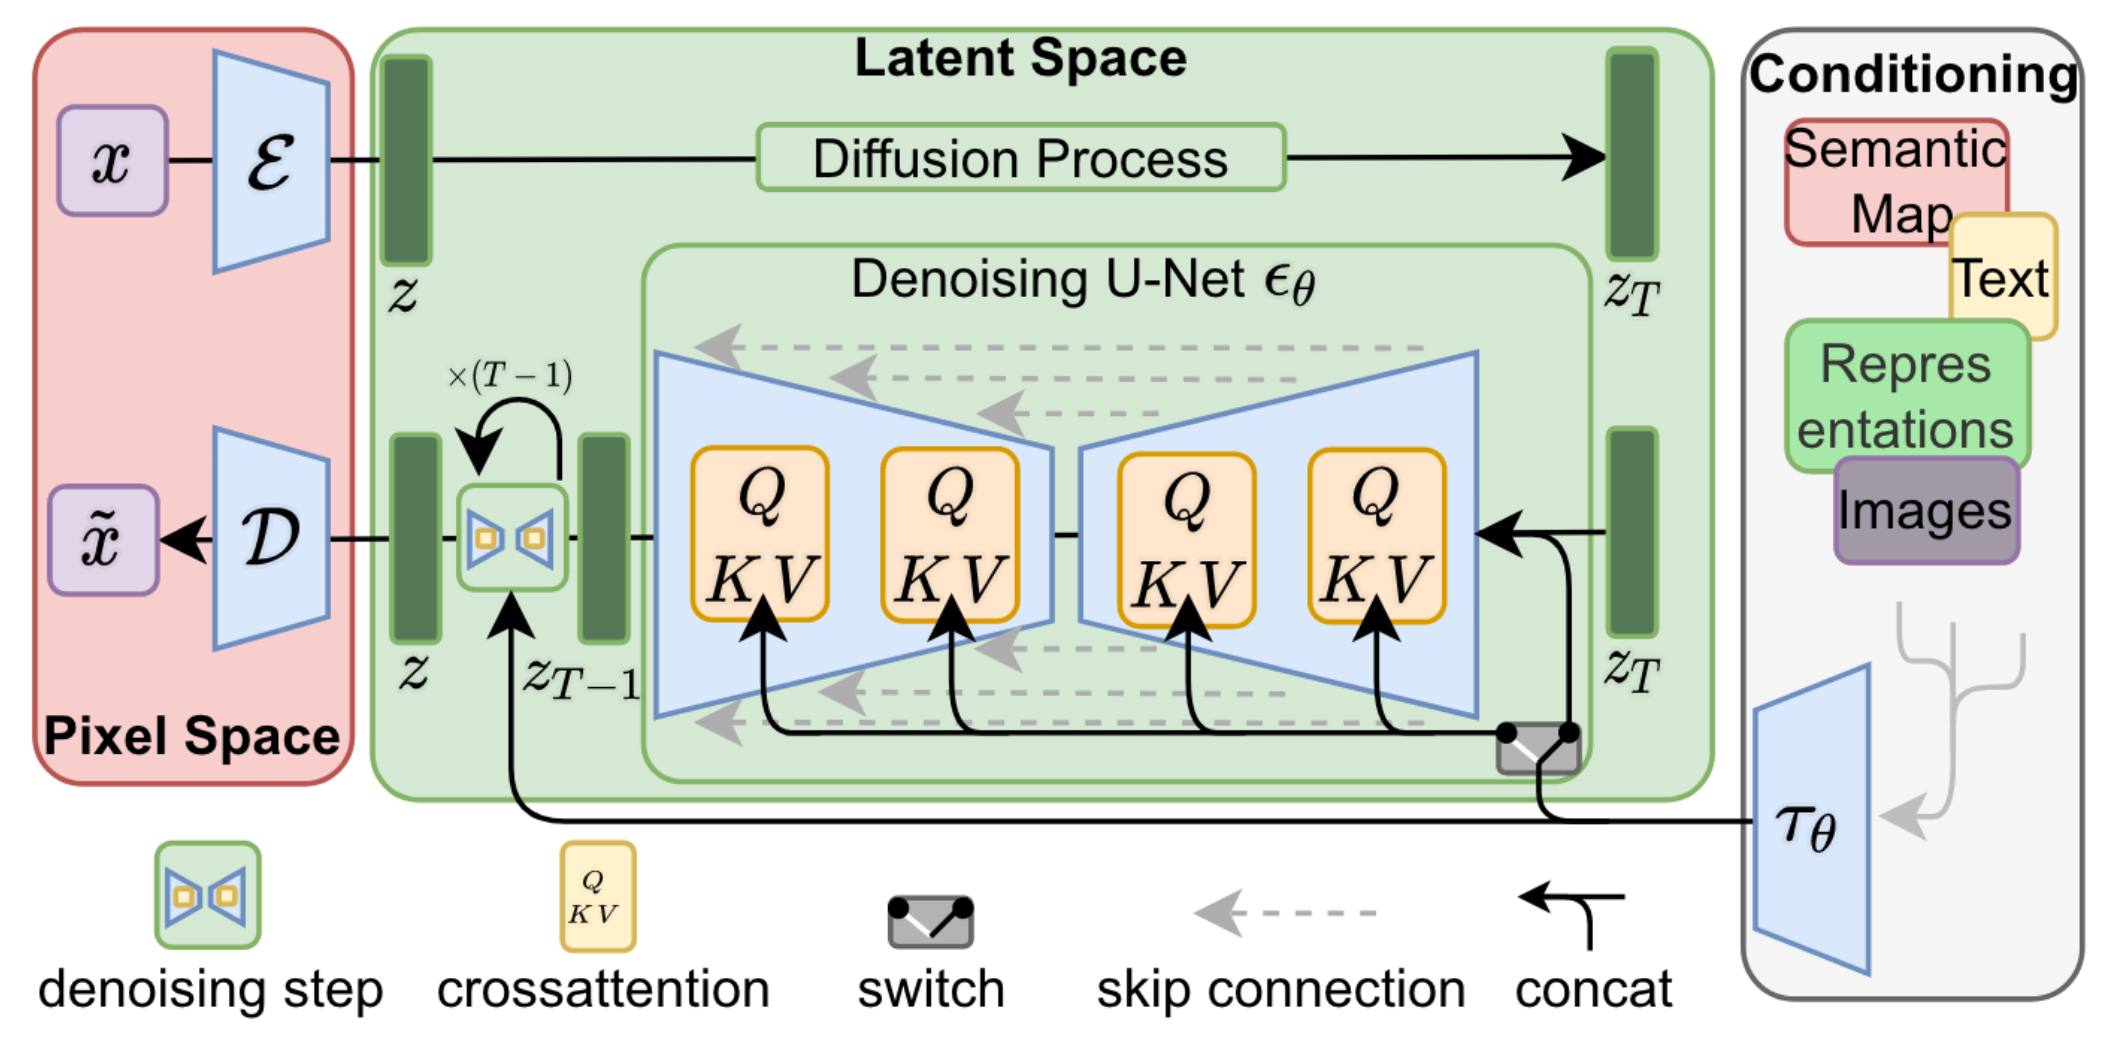
\includegraphics[width=.8\textwidth]{LDM.png}
  \caption[LDM Architektur]{LDM-Architektur: \emph{Diffusion} mittels \emph{U-Net} im durch den \emph{Encoder} $\mathcal{E}$ erzeugten \emph{latenten} Raum. Rekonstruktion in die ursprüngliche Darstellung erfolgt durch den \emph{Decoder} $\mathcal{D}$. \cite{rombach_high-resolution_2022}}
  \label{fig:LDM}
\end{figure} 

Durch das vorausgehende Training eines \emph{Variational Autoencoders} \cite{kingma_auto-encoding_2022} gemäß \cite{esser_taming_2021} wird der \emph{latente} Raum für den \emph{Diffusions}-prozess erzeugt. Dabei transformiert der resultierende \emph{Encoder} $\mathcal{E}$ ein RGB-Bild $x \in \mathbb{R}^{H \times W \times 3}$ in seine \emph{latente} Darstellung $z \in \mathbb{R}^{h \times w \times c}$, dargestellt als $z=\mathcal{E}(x)$. Nach dem \emph{Rückwärtsdiffusions}-prozess generiert ein \emph{Decoder} $\mathcal{D}$ das Bild zurück, wobei $\tilde{x}=\mathcal{D}(z)=\mathcal{D}(\mathcal{E}(x))$. \cite{rombach_high-resolution_2022}

Dank der niedrigen Dimensionalität und Kompression des \emph{latenten} Raumes eignet sich der \emph{Diffusions}prozess besser für \emph{likelihood}-basierte generative Modelle als die Verwendung der ursprünglichen Pixelwerte. Dies liegt daran, dass semantisch wichtige Informationen stärker hervorgehoben werden und der Rechenaufwand effizienter gestaltet wird. Das zugrundeliegende \emph{U-Net} \cite{ronneberger_u-net_2015} verwendet hauptsächlich \emph{2D-Konvolutionsschichten}, um die Bildverarbeitung zu optimieren. \cite{rombach_high-resolution_2022}

Um eine von $y$ abhängige Generierung zu ermöglichen, muss das Netzwerk $\epsilon_\theta\left(z_t, t, y\right)$ konditioniert werden. Dazu wird das verwendete \emph{U-Net} durch \emph{Cross Attention} \cite{vaswani_attention_2017} erweitert. Ein spezifischer \emph{Encoder} $\tau_\theta$ passt sich an verschiedene Eingabemodalitäten an und erstellt eine Repräsentation $T_\theta(y) \in \mathbb{R}^{M \times d_\tau}$. Diese Repräsentation wird mittels \emph{Cross Attention} auf die Schichten des \emph{U-Net} angewendet. Die dabei verwendete Aufmerksamkeitsfunktion ist durch $\operatorname{Attention}(Q, K, V)=\operatorname{softmax}\left(\frac{Q K^T}{\sqrt{d}}\right)$ definiert, wobei  $Q=W_Q^{(i)} \cdot \varphi_i\left(z_t\right), K=W_K^{(i)} \cdot \tau_\theta(y), V=W_V^{(i)} \cdot \tau_\theta(y)$ entsprechend gegeben sind. Die zugehörige Verlustfunktion wird im Folgenden beschrieben. \cite{rombach_high-resolution_2022}

\begin{equation}
L_{L D M}:=\mathbb{E}_{\mathcal{E}(x), y, \epsilon \sim \mathcal{N}(0,1), t}\left[\left\|\epsilon-\epsilon_\theta\left(z_t, t, \tau_\theta(y)\right)\right\|_2^2\right]
\end{equation}

\subsection{Clap}

\emph{Large-Scale Contrastive Language-Audio Pretraining} (\emph{Clap}) \cite{wu_large-scale_2023} erschafft, mittels \emph{Contrastive Learning} eine Vorverarbeitung auf Sprach-Audio-Daten durchzuführen. Ziel ist es, eine \emph{latente} Repräsentation für Audio zu erstellen. Inspiriert wurde dieses Modell von \emph{Contrastive Language-Image Pretraining} (\emph{CLIP}) \cite{radford_learning_2021}, welches den Zusammenhang zwischen Bild- und Textdaten in ähnlicher Weise lernt. Analog zum bildlichen Kontext weisen Audio und Text überlappende Informationen auf. \cite{wu_large-scale_2023}

Das \emph{Contrastive Learning}-Modell wurde mit dem spezifisch veröffentlichten Datensatz \emph{LAION-Audio-630K} trainiert. Dieser umfasst $633,526$ Paare aus Text und Audio ($X_i^a$, $X_i^t$), die aus verschiedenen Online-Quellen stammen. Dazu gehören menschliche Stimmen, Naturklänge und Audioeffekte. Zusätzlich wurden die Datensätze \emph{AudioCaps+Clotho} \cite{kim_audiocaps_2019} \cite{drossos_clotho_2019} und \emph{AudioSet} \cite{gemmeke_audio_2017} verwendet. Alle Audiodateien wurden in ein \emph{Mono}-Signal umgewandelt und haben eine Abtastrate von 48kHz. \cite{wu_large-scale_2023}

\begin{figure}[h]
  \centering
  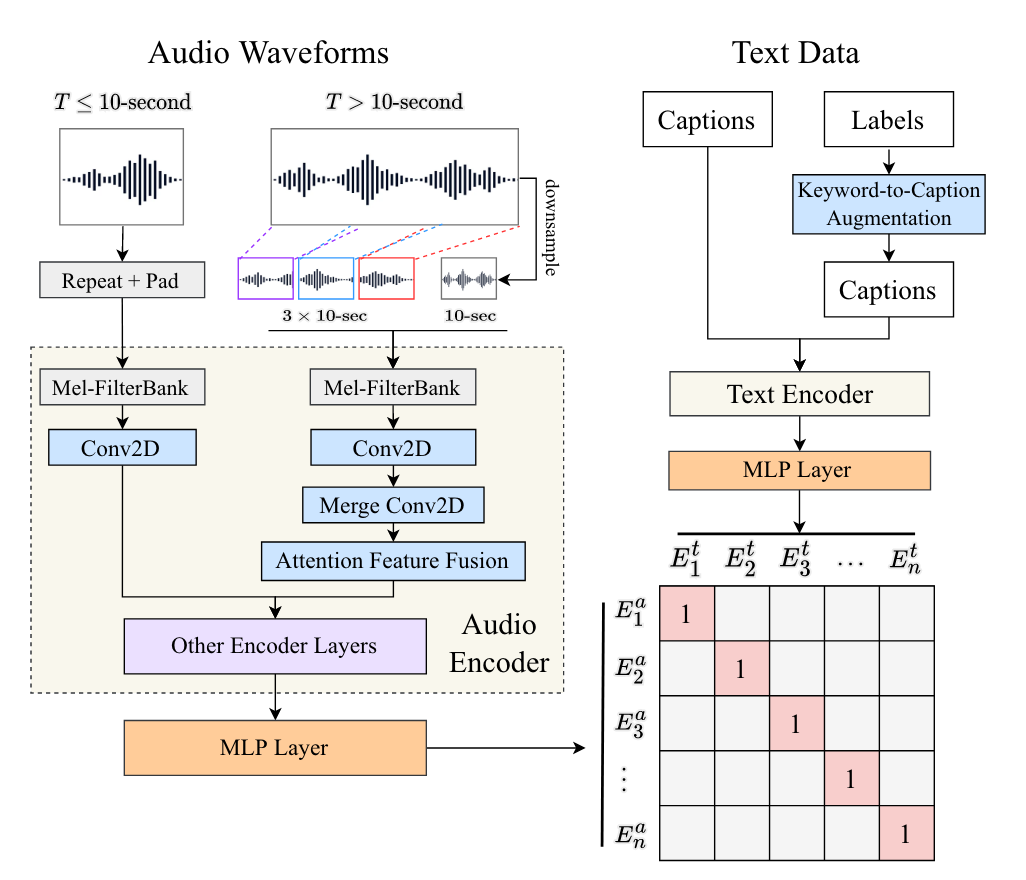
\includegraphics[width=.7\textwidth]{Clap.png}
  \caption[Clap Architektur]{CLAP-Architektur für \emph{latente} Repräsentation von Text-Audio-Paaren: Der Audio-\emph{Encoder} verarbeitet Signale variabler Länge und adaptiert sie für das \emph{MLP}. Der Text-\emph{Encoder} behandelt textuelle Eingaben; bei Verwendung von Labeln erfolgt zuerst eine Umschreibung. \cite{wu_large-scale_2023}}
  \label{fig:Clap}
\end{figure} 

Die Modellarchitektur, dargestellt in Abbildung \ref{fig:Clap}, generiert Embeddings $E_i^a$ und $E_i^t$ für die Audio- $X_i^a$ und Texteingabe $X_i^t$. Hierfür wird zunächst ein Encoder $f(\cdot)$ eingesetzt, dessen Ergebnis anschließend durch ein zweischichtiges \emph{Multi-Layer-Perceptron} (\emph{MLP}) mit \emph{ReLU} \cite{agarap_deep_2019} als Aktivierungsfunktion weiterverarbeitet wird. \cite{wu_large-scale_2023}

\begin{equation}
     E_i^a = M L P_{\text{audio}}\left(f_{\text{audio}}\left(X_i^a\right)\right)
\end{equation}
\begin{equation}
    E_i^t = M L P_{\text{text}}\left(f_{\text{text}}\left(X_i^t\right)\right)
\end{equation}

Um die Rechenzeit bei längeren Audiosignalen zu minimieren, wurde ein Ansatz entwickelt, der es ermöglicht, Audioeingaben unterschiedlicher Länge in konstanter Zeit zu verarbeiten. Dabei werden sowohl globale als auch lokale Signalinformationen berücksichtigt. Bei Signalen unter 10 Sekunden wird das Signal dreifach wiederholt und mit Nullen ergänzt, bis es 10 Sekunden erreicht. Für Signale über 10 Sekunden werden vier Eingaben erstellt: Einmal wird das gesamte Signal auf 10 Sekunden \emph{downgesampled} und zusätzlich werden drei zufällige 10-Sekunden-Abschnitte aus verschiedenen Signalbereichen entnommen. Der Audio-\emph{Encoder} kombiniert anschließend diese globalen und lokalen Daten, um die relevanten Informationen zu extrahieren. \cite{wu_large-scale_2023}

Einige der genutzten Datensätze enthalten für Audiosignale lediglich Keywords oder Tags statt vollständiger Beschreibungen. Um diesem Mangel zu begegnen, wurde das \emph{T5} \cite{raffel_exploring_2020} \emph{Language}-Modell verwendet, um aus diesen Stichworten und Tags umfassende Beschreibungen zu erstellen. Zusätzlich wurden die generierten Beschreibungen von Voreingenommenheiten befreit, wie zum Beispiel durch das Entfernen geschlechtsspezifischer Verzerrungen (eng. \emph{gender de-biasing}). \cite{wu_large-scale_2023}

Die gleiche Verlustfunktion mit einem Temperaturparameter $\tau$, wie in \emph{Clip} \cite{radford_learning_2021}, wurde in den MLPs verwendet \cite{wu_large-scale_2023}.

\begin{equation}
L=\frac{1}{2 N} \sum_{i=1}^N\left(\log \frac{\exp \left(E_i^a \cdot E_i^t / \tau\right)}{\sum_{j=1}^N \exp \left(E_i^a \cdot E_j^t / \tau\right)}+\log \frac{\exp \left(E_i^t \cdot E_i^a / \tau\right)}{\sum_{j=1}^N \exp \left(E_i^t \cdot E_j^a / \tau\right)}\right)
\end{equation}

Als Audio-\emph{Encoder} wurden die Modelle \emph{PANN} \cite{kong_panns_2020}, basierend auf einem \emph{Convolutional Neural Network} (CNN), und \emph{HTSAT} \cite{chen_hts-at_2022}, basierend auf einem \emph{Transformer}-Modell, evaluiert. Für den Text-\emph{Encoder} wurden der Text-\emph{Encoder} von \emph{Clip} \cite{radford_learning_2021}, \emph{Bert} \cite{devlin_bert_2019}, und \emph{RoBERTa} \cite{liu_roberta_2019} ebenfalls ausgewertet. \cite{wu_large-scale_2023}

Das trainierte Modell eignet sich sowohl für die Audio-Klassifikation als auch zur Bestimmung eines zugehörigen Audiosignals für einen gegebenen Text $(T\rightarrow A)$ \cite{wu_large-scale_2023}. Insbesondere für die Klangsynthese ist die Konversion von Text zu Audio von großer Relevanz. Die Untersuchungsergebnisse, die durch die Kombination verschiedener \emph{Encoder} aus Tabelle \ref{tab:Clap} erzielt wurden, verdeutlichen, dass \emph{HTSAT} \cite{chen_hts-at_2022} als Audio-\emph{Encoder} in Kombination mit \emph{Bert} \cite{devlin_bert_2019} oder \emph{RoBERTa} \cite{liu_roberta_2019} als Text-\emph{Encoder}, abhängig vom verwendeten Datensatz, die optimalsten Ergebnisse erbrachte. \cite{wu_large-scale_2023}

\begin{table}[h]
  \centering
\begin{tabular}{lcc|cc}
\hline \multirow{2}{*}{ Model } & \multicolumn{2}{c|}{ AudioCaps $(\mathrm{mAP} @ 10)$} & \multicolumn{2}{c}{ Clotho (mAP@ 10) } \\
\cline { 2 - 5 } & $\mathrm{A} \rightarrow \mathrm{T}$ & $\mathrm{T} \rightarrow \mathrm{A}$ & $\mathrm{A} \rightarrow \mathrm{T}$ & $\mathrm{T} \rightarrow \mathrm{A}$ \\
\hline PANN+CLIP Trans. & 4.7 & 11.7 & 1.9 & 4.4 \\
PANN+BERT & 34.3 & 44.3 & 10.8 & 17.7 \\
PANN+RoBERTa & 37.5 & 45.3 & 11.3 & 18.4 \\
HTSAT+CLIP Trans. & 2.4 & 6.0 & 1.1 & 3.2 \\
HTSAT+BERT & 43.7 & 49.2 & $\mathbf{1 3 . 8}$ & $\mathbf{2 0 . 8}$ \\
HTSAT+RoBERTa & $\mathbf{4 5 . 7}$ & $\mathbf{5 1 . 3}$ & $\mathbf{1 3 . 8}$ & 20.4 \\
\hline
\end{tabular}
\caption[Encoder CLAP]{Evaluation der Encoder \cite{wu_large-scale_2023}}
  \label{tab:Clap}
\end{table}

\subsection{AudioLDM}
\label{sec:AudioLDM}

\emph{AudioLDM} \cite{liu_audioldm_2023} wurde entwickelt, um sowohl die Synthese von Text zu Audio als auch die textgesteuerte Audio-Manipulation mittels \emph{Latenter Diffusion} \cite{rombach_high-resolution_2022} durchzuführen. Es bietet den Vorteil qualitativ hochwertiger Ergebnisse bei minimalem Rechenaufwand. Während \emph{Diffsound} \cite{yang_diffsound_2023} Audio-Text-Paare für Trainingszwecke nutzt, hat \emph{AudioLDM} nachgewiesen, dass durch die Verwendung einer \emph{CLAP}-Repräsentation \cite{wu_large-scale_2023} hochwertige Resultate erlangt werden können. \cite{liu_audioldm_2023}.

Die Entscheidung, Natürliche Sprache anstelle von Labels für Eingabe und Konditionierung zu nutzen, wurde getroffen, um akustische Merkmale in einer flexibleren, deskriptiveren und präziseren Weise darstellen zu können. Frühere Ansätze im Bereich Text-zu-Audio (TTA) waren durch das Fehlen großer Mengen an qualitativ hochwertigen Audio-Text-Daten limitiert \cite{liu_separate_2022}. Obwohl Methoden der Textvorverarbeitung \cite{gemmeke_audio_2017, yang_diffsound_2023} versuchten, dieses Problem zu adressieren, konnten sie die komplexen Beziehungen zwischen Klangereignissen nicht vollständig erfassen, was zu einer Beeinträchtigung der Generierungsleistung führte. Das Modell \emph{AudioLDM} begegnete dieser Herausforderung, indem es im Training ausschließlich auf Audiodaten zurückgriff und somit überzeugendere Ergebnisse im Vergleich zu Ansätzen mit gepaarten Audio-Text-Daten erzielte \cite{liu_audioldm_2023}


\begin{figure}[h]
  \centering
  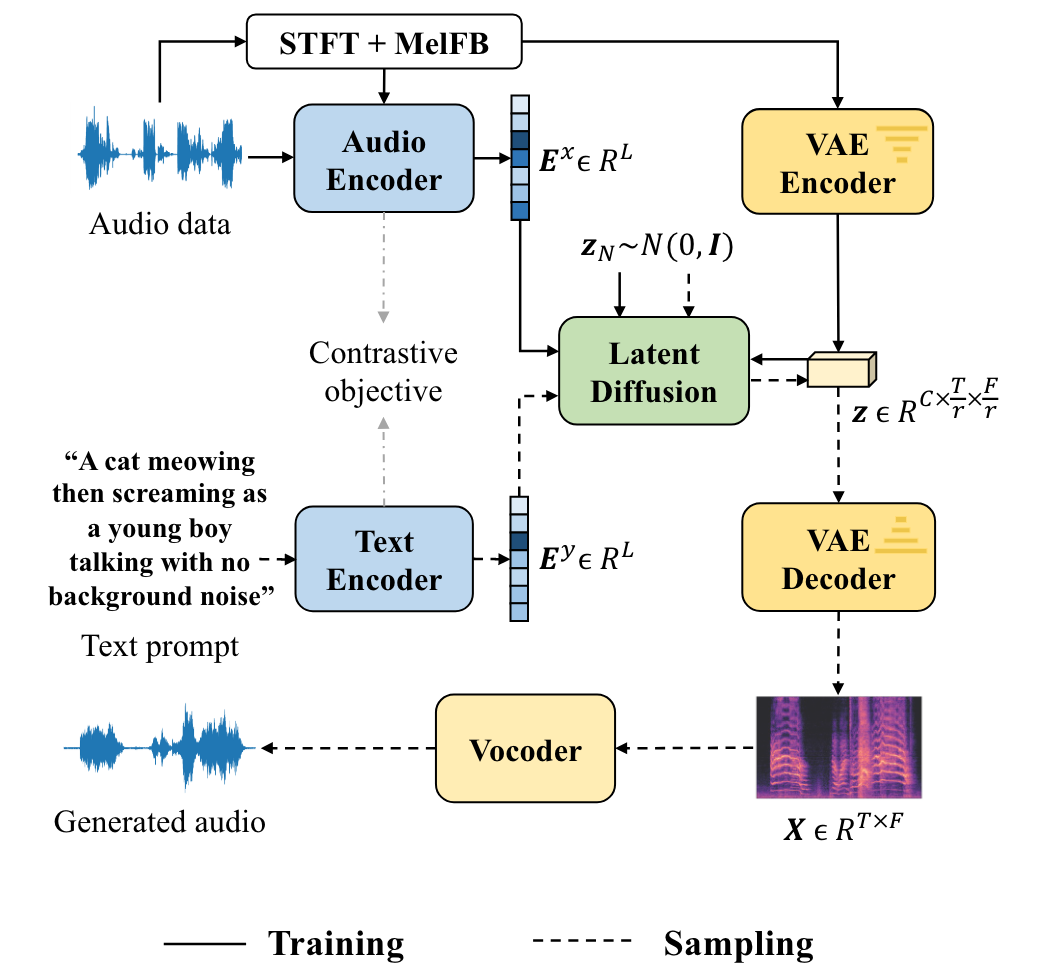
\includegraphics[width=.6\textwidth]{AudioLDM.png}
  \caption[AudioLDM Architektur]{Architektur von AudioLDM für Text-zu-Audio-Generierung: Die \emph{VAE}-\emph{Encoder} und \emph{Decoder} bilden auf Grundlage von Spektogrammen die \emph{latente} Repräsentation, die mittels \emph{Diffusion} modifiziert wird. Text- und Audio-\emph{Encoder} dienen der Konditionierung, während der \emph{Vocoder} ein Audiosignal aus dem Spektogramm generiert. \cite{liu_audioldm_2023}}
  \label{fig:AudioLDM}
\end{figure} 

Die in Abbildung \ref{fig:AudioLDM} dargestellte Architektur integriert mehrere Komponenten: Einen \emph{VAE} \cite{kingma_auto-encoding_2022}, welcher Mel-Spektrogramme in einen \emph{latenten} Raum transformiert; einen nach dem \emph{CLAP}-Prinzip \cite{wu_large-scale_2023} entworfenen Audio- und Text-\emph{Encoder} zur Erzeugung von Embeddings, die zur Konditionierung des \emph{LDMs} dienen; einen \emph{LDM}, der die inhärente Verteilung modelliert; sowie einen \emph{Vocoder}, der das generierte Spektrogramm in ein hörbares Audiosignal konvertiert. \cite{liu_audioldm_2023}

Die \emph{CLAP}-Module erzeugen Embeddings sowohl für Text, repräsentiert durch $\boldsymbol{E}^y \in \mathbb{R}^L$, als auch für Audio, dargestellt durch $\boldsymbol{E}^x \in \mathbb{R}^L$. In diesem Kontext steht $x$ für eine Audioprobe und $y$ für eine Textbeschreibung. Die Funktionen $f_{\text {text }}(\cdot)$ und $f_{\text {audio }}(\cdot)$ agieren hierbei als \emph{Encoder}. Als Audio-\emph{Encoder} kam \emph{HTSAT} \cite{chen_hts-at_2022} zum Einsatz, während für den Text-\emph{Encoder} \emph{RoBERTa} \cite{liu_roberta_2019} verwendet wurde. Während des Trainingsprozesses des \emph{LDMs} fungierte $\boldsymbol{E}^x$ des jeweiligen Trainingsdatenpunkts als Konditionierungselement, wohingegen $\boldsymbol{E}^y$ zur Generierung des gewünschten Signals herangezogen wurde \cite{liu_audioldm_2023}.

Der für den \emph{LDM} verwendete \emph{Latentraum}, beschrieben durch $\boldsymbol{z} \in \mathbb{R}^{C \times \frac{T}{r} \times \frac{F}{r}}$, wurde mittels eines \emph{VAE} auf der Grundlage von Spektrogrammen trainiert. In dieser Darstellung bezeichnet $r$ das \emph{Kompressionsniveau}. Die Variablen $T$ und $F$ repräsentieren die Zeit- und Frequenzdimensionen, während $C$ die Anzahl der Kanäle angibt. Ein gegebenes Audiosignal wird durch die \emph{STFT}-Methode (siehe Referenz \ref{sec:music_math}) in ein Spektrogramm $\boldsymbol{X} \in \mathbb{R}^{T \times F}$ überführt. Im Generierungsprozess wird aus der \emph{latenten} Variable $\hat{\boldsymbol{z}}_o$ ein Spektrogramm $\hat{\boldsymbol{X}}$ erzeugt. Dieses generierte Spektrogramm wird anschließend durch den \emph{Vocoder}, welcher auf \emph{HiFi-GAN} \cite{kong_hifi-gan_2020} basiert, in ein Audiosignal $\hat{x}$ konvertiert. \cite{liu_audioldm_2023}

Das konzeptuelle Modell \emph{LDM} verfolgt die Absicht, die fundamentale Verteilung $q\left(\boldsymbol{z}0 \mid \boldsymbol{E}^y\right)$ durch die Annäherung an $p\theta\left(\boldsymbol{z}_0 \mid \boldsymbol{E}^y\right)$ zu repräsentieren. In diesem Kontext wurden sowohl die Verlustfunktion als auch der Rückwärtsprozess entsprechend definiert: \cite{liu_audioldm_2023}

\begin{equation}
    L_n(\theta)=\mathbb{E}_{\boldsymbol{z}_0, \boldsymbol{\epsilon}, n}\left\|\boldsymbol{\epsilon}-\boldsymbol{\epsilon}_\theta\left(\boldsymbol{z}_n, n, \boldsymbol{E}^x\right)\right\|_2^2
\end{equation}
\begin{equation}
    p_\theta\left(\boldsymbol{z}_{n-1} \mid \boldsymbol{z}_n, \boldsymbol{E}^y\right)=\mathcal{N}\left(\boldsymbol{z}_{n-1} ; \boldsymbol{\mu}_\theta\left(\boldsymbol{z}_n, n, \boldsymbol{E}^y\right), \boldsymbol{\sigma}_n^2 \boldsymbol{I}\right)
\end{equation}
\begin{equation}
    p_\theta\left(\boldsymbol{z}_{0: N} \mid \boldsymbol{E}^y\right)=p\left(\boldsymbol{z}_N\right) \prod^N p_\theta\left(\boldsymbol{z}_{n-1} \mid \boldsymbol{z}_n, \boldsymbol{E}^y\right) \\
\end{equation}

Der Erwartungswert wird wie folgt parametrisiert und ergibt sich aus dem im Rückwärtsverfahren ermittelten Rauschen: $\boldsymbol{\epsilon}_\theta\left(\boldsymbol{z}_n, n, \boldsymbol{E}^y\right)$ \cite{liu_audioldm_2023}.

\begin{equation}
    \boldsymbol{\mu}_\theta\left(\boldsymbol{z}_n, n, \boldsymbol{E}^y\right)=\frac{1}{\sqrt{\alpha_n}}\left(\boldsymbol{z}_n-\frac{\beta_n}{\sqrt{1-\bar{\alpha}_n}} \boldsymbol{\epsilon}_\theta\left(\boldsymbol{z}_n, n, \boldsymbol{E}^y\right)\right)
\end{equation}

Ferner wurde nachgewiesen, dass der \emph{Cross-Attention}-Mechanismus gemäß \cite{rombach_high-resolution_2022} entbehrlich ist \cite{liu_audioldm_2023}.

\subsection{AudioLDM2}

\emph{AudioLDM2} \cite{liu_audioldm2_2023} baut auf den erarbeiteten Konzepten von \emph{AudioLDM} \cite{liu_audioldm_2023} auf und verspricht durch eine neuartige Architektur (siehe Abbildung \ref{fig:AudioLDM2}) in Verbindung mit innovativen Konzepten verbesserte Resultate in der Audiogenerierung mittels neuronaler Netze. Die treibende Kraft hinter dieser Entwicklung war die Erkenntnis, dass im Bereich der Audiosynthese zwar verschiedene Modelle für unterschiedliche Anwendungen wie Spracherzeugung, Musikgenerierung und Klangsynthese existieren, diese jedoch häufig so spezifisch und beschränkt für eine bestimmte Aufgabe oder Domäne entwickelt werden, dass ihre Anwendbarkeit in einem übergeordneten Kontext limitiert ist. Das vorgestellte Modell verfolgt das Ziel, diese diversen spezifischen Herausforderungen in einem einzigen Modell zu integrieren. Zu diesem Zweck wurde eine Audio-Repräsentation namens \emph{language of audio} (\emph{LOA}) konzipiert, die sich effizient über verschiedene Domänen und Modalitäten, wie Text, Audio und verschiedene Medien, generalisieren lässt. Auf Basis dieser Repräsentation wurde ein \emph{Latente-Diffusion}-Modell trainiert, um die Audiosynthese zu realisieren. \cite{liu_audioldm2_2023}

\begin{figure}[h]
  \centering
  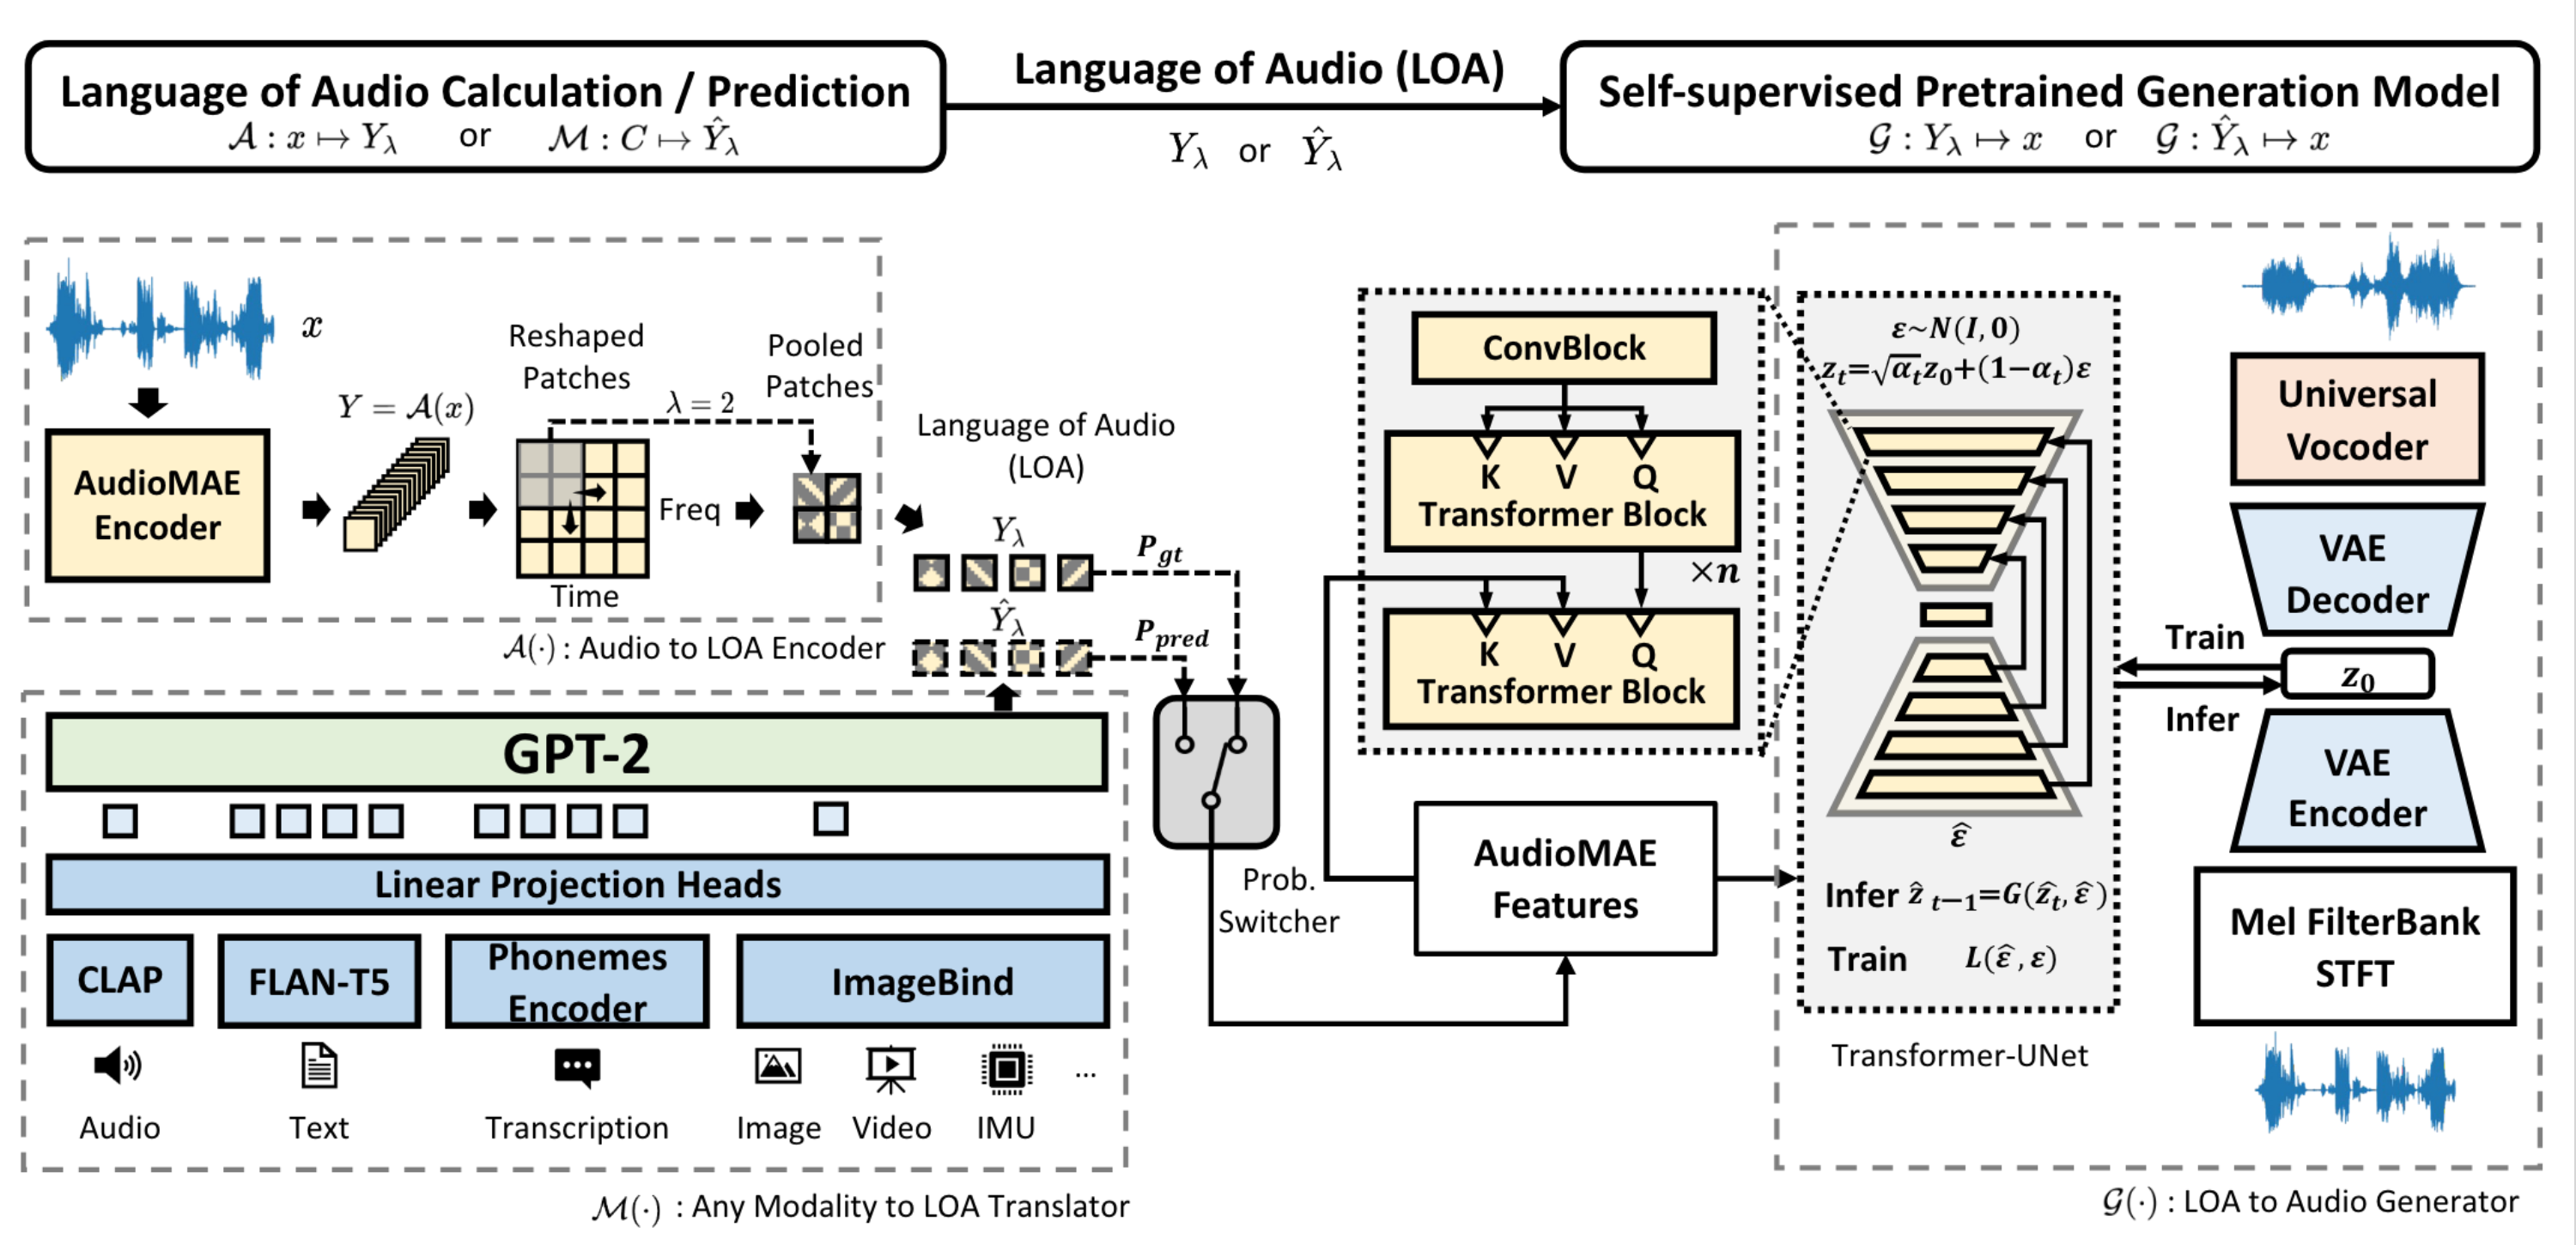
\includegraphics[width=1.0\textwidth]{AudioLDM2.png}
  \caption[AudioLDM2 Architektur]{Architektur von AudioLDM2: Das \emph{Diffusions}-netz integriert \emph{U-Net} und \emph{Transformer}-Konzepte und operiert auf der \emph{latenten} Repräsentation von Spektogrammen. Die Konditionierung basiert auf der \emph{LOA}-Repräsentation, abgeleitet von \emph{AudioMAE}-Informationen. Diese kann entweder durch den Audio-zu-\emph{LOA} Encoder oder den \emph{Any Modality}-zu-\emph{LOA} Konverter gewonnen werden. \cite{liu_audioldm2_2023}}
  \label{fig:AudioLDM2}
\end{figure} 

Die Synthese eines Audiosignals $x \in \mathbb{R}^{L_s}$, wobei $L_s$ die Dauer des Signals in Sekunden angibt, kann als Funktion $\mathcal{H}: C \mapsto x$ im Hypothesenraum $\mathcal{H}$ dargestellt werden. In dieser Funktion stellt $C$ die Eingabe dar, auf deren Basis das Signal generiert wird. Diese Eingabe kann sowohl Text als auch diverse Medienformate umfassen. Das Erlernen dieser Funktion stellt aufgrund der signifikanten Unterschiede in den Verteilungen von $C$ und $x$ eine besondere Herausforderung dar. Ein vorgeschlagener Lösungsweg besteht in einer Abstraktion durch \emph{LOA}. Die Darstellung eines Audiosignals im \emph{LOA}-Format wird als $Y=\mathcal{A}(x)$ definiert, wobei $\mathcal{A}$ einen Audio-zu-LOA-\emph{Encoder} darstellt. $\mathcal{A}$ kann entweder durch vordefinierte Regeln definiert oder mittels \emph{self-supervised learning} \cite{tan_regeneration_2023} trainiert werden. Um verschiedenste Eingabeformate zu unterstützen und in \emph{LOA} zu konvertieren, wurde der Übersetzer \emph{any modality to LOA translator} $\mathcal{M}$ als $\hat{Y}=\mathcal{M}(C)$ definiert. Infolgedessen kann die Signalgenerierungsfunktion entsprechend formuliert werden. \cite{liu_audioldm2_2023}

\begin{equation}
    \mathcal{H}_0=\mathcal{G} \circ \mathcal{M}: C \mapsto \hat{Y} \mapsto x
\end{equation}

Hierbei extrahiert $\mathcal{G}$ ein Audiosignal aus der \emph{LOA}-Repräsentation. Falls $\mathcal{M}$ durch $\mathcal{A}$ ersetzt wird  (wie in Gleichung \ref{eqn:h1} gezeigt), tritt nur $x$ als Trainingsdaten für $\mathcal{G}$ auf. Dementsprechend kann $\mathcal{G}$ \emph{self-supervised} ohne den Einsatz von Labels trainiert werden, wodurch das Problem einer geringen Anzahl an gelabelten Audiopaaren umgangen wird. \cite{liu_audioldm2_2023}

\begin{equation}
\label{eqn:h1}
    \mathcal{H}_0=\mathcal{G} \circ \mathcal{A}: C \mapsto Y \mapsto x
\end{equation}

Um eine vielfältige Audio-Repräsentation $Y$ für Sprache, Musik und Soundeffekte zu erstellen, sollte diese in der Lage sein, sowohl semantische als auch akustische Informationen zu erfassen. Zur Erfüllung dieser Kriterien wurde für den \emph{Audio zu LOA}-\emph{Encoder} das mittels \emph{self-supervised} Verfahren vortrainierte Modell \emph{AudioMAE} \cite{huang_masked_2023} herangezogen. Das Modell trainiert eine Repräsentation von ungelabelten Audiosignalen mithilfe eines \emph{Encoder}-\emph{Decoder}-Ansatzes. Hierbei werden dem \emph{Encoder} \emph{Mel}-Spektrogramme mit maskierten Bereichen übergeben, welche der \emph{Decoder} anschließend zu rekonstruieren versucht. Nachdem die Repräsentation $Y$ generiert wurde, kann diese durch den Einsatz von \emph{average-max pooling} \cite{liu_simple_2023} weiter zu $Y_\lambda$ verfeinert werden. \cite{liu_audioldm2_2023}

Das Erlernen von $\mathcal{G}$ wurde in Anlehnung an \emph{AudioLDM} \cite{liu_audioldm_2023} mittels \emph{Latenter Diffusion} \cite{rombach_high-resolution_2022} durchgeführt (vgl. \ref{sec:AudioLDM}). Der \emph{Diffusions}-vorgang erreignet sich in einem \emph{latenten} Raum, der mittels eines \emph{VAE} \cite{kingma_auto-encoding_2022} erlernt wurde. Die \emph{Diffusion} findet nicht direkt auf $Y$ statt, da sich \emph{AudioMAE} nicht in erster Linie auf den Erhalt der Qualität während des Rekonstruktionsvorgangs konzentriert. Ein \emph{VAE} hingegen kennzeichnet sich durch eine überlegene Rekonstruktionsfähigkeit und ein intensiveres Kompressionsverhältnis. Während \emph{AudioMAE} primär semantische Aspekte hervorhebt, legt der \emph{VAE} sein Augenmerk verstärkt auf akustische Details. \cite{liu_audioldm2_2023}

Die durch den \emph{VAE} generierte \emph{latente} Repräsentation $z$ wird mittels eines \emph{Encoders}, der Downsampling verwendet, und eines \emph{Decoders}, der Upsampling einsetzt, erlernt. Ein gegebenes Spektrogramm $X$ wird in $z$ umgewandelt und gemäß $\mathcal{V}: X \mapsto z \mapsto \hat{X}$ rekonstruiert. Aus $\hat{X}$ kann mithilfe eines vortrainierten vortrainierten \emph{HiFiGAN} \cite{kong_hifi-gan_2020} ein Audiosignal generieren. Die Optimierung des \emph{VAE} basiert auf den Differenzen zwischen $X$ und $\hat{X}$. \cite{liu_audioldm2_2023}

Der Vorwärtsprozess des \emph{LDM} im \emph{latenten} Raum mit dem Hyperparameter $\beta_t \in[0,1]$ ist wie folgt definiert \cite{liu_audioldm2_2023}:
\begin{equation}
    q\left(z_t \mid z_{t-1}\right)=\sqrt{1-\beta_t} z_{t-1}+\sqrt{\beta_t} \epsilon_t, t \in 2, \ldots, T
\end{equation}

Der Rückwärtsprozess hingegen ist definiert als \cite{liu_audioldm2_2023}:
\begin{equation}
q\left(z_t \mid z_0\right)=\sqrt{\alpha_t} z_0+\sqrt{1-\alpha_t} \epsilon_t
\end{equation}

Die zugehörige Verlustfunktion lautet \cite{liu_audioldm2_2023}:
\begin{equation}
\operatorname{argmin}_\phi\left[\mathbb{E}_{z_0, Y, t \sim\{1, \ldots, T\}}\left\|\mathcal{G}\left(\sqrt{\alpha_t} z_0+\sqrt{1-\alpha_t} \epsilon_t, t, Y ; \phi\right)-\epsilon_t\right\|\right]
\end{equation}

Für $\mathcal{G}$ kam ein \emph{Transformer-UNet} (\emph{T-UNET}) zum Einsatz. Dieses Netzwerk vereint einen \emph{Encoder}, der Downsampling nutzt, mit einem \emph{Decoder}, der Upsampling einsetzt. Im Anschluss an einen \emph{Konvolutions}-Block werden zudem \emph{Transformer}-Blöcke eingebunden. \cite{liu_audioldm2_2023}

Das Modell $\mathcal{M}$ ist von Bedeutung, da während der Inferenz $\mathcal{A}$ nicht verfügbar ist. Zur Generierung von $\hat{Y}$ ist ein alternatives Modell $\mathcal{M}_\theta: C \rightarrow \hat{Y}$ erforderlich. Dabei stellt $\theta$ die anlernbaren Parameter dar. Um der Ausgabe des \emph{AudioMAE} optimal zu entsprechen, wurde dieses Problem als Aufgabe der Sprachmodellierung definiert. Als Basis für dieses Modell dient der \emph{Generative Pre-trained Transformer 2} (\emph{GPT-2}) \cite{alec_radford_jeff_wu_rewon_child_david_luan_dario_amodei_ilya_sutskever_language_2019}. Dieser wurde mittels eines \emph{unsupervised} Verfahrens auf einem umfangreichen Textdatensatz trainiert. Sein Hauptziel ist die Bewältigung von Aufgaben im Kontext des \emph{Natural Language Processing} (\emph{NLP}), wie Textvervollständigung, Frage-Antwort-Systeme oder Sprachübersetzung. Das Modell \emph{GPT-2} wurde spezifisch für den Einsatz in \emph{AudioLDM2} mittels \emph{teacher forcing} \cite{kolen_field_2001} verfeinert.Gegeben ein Datensatz $C$, wird das Modell durch die Maximierung der Likelihood optimiert. $C$ kann diverse Daten repräsentieren, darunter Audio, Text, Phoneme oder visuelle Daten. Zur Extraktion essenzieller Merkmale kommt ein \emph{Mischung von Experten}-Ansatz (engl. \emph{mixture of experts}) \cite{masoudnia_mixture_2014} zum Einsatz, wodurch ein vielfältiges Informationsspektrum zugänglich gemacht wird. Ein \emph{Linearer Adapter} (engl. \emph{linear adaptor}) dient dazu, sämtliche Merkmale auf die einheitliche Dimension $D$ zu bringen. Verschiedenste Systeme können zur Extraktion dieser Merkmale genutzt werden. \cite{liu_audioldm2_2023}

Zur Nutzung von Text als Kondition $C$ kamen sowohl \emph{CLAP} \cite{wu_large-scale_2023} als auch \emph{FLAN-T5} \cite{chung_scaling_2022} zum Einsatz. Da \emph{CLAP} Schwierigkeiten bei der angemessenen Verarbeitung temporaler und semantischer Informationen aufwies, fungierte \emph{FLAN-T5} zusätzlich als zusätzlicher \emph{Encoder}. Des Weiteren diente \emph{CLAP} der Generierung von Paraphrasen für Audiosignale, welche ursprünglich keine entsprechenden Umschreibungen besaßen, wie es bei Text-zu-Sprach-Aufgaben vorkommt. Ein weiterer in der Arbeit implementierter \emph{Encoder} ist der \emph{Phoneme Encoder}. Dieser wurde speziell konzipiert, um Informationen über Phoneme, die kleinsten sprachlichen Einheiten, zu kodieren. Für die Kodierung visueller Daten wurde \emph{ImageBind} \cite{girdhar_imagebind_2023} eingesetzt. \cite{liu_audioldm2_2023}

Während des Finetunings entschied ein probabilistischer Mechanismus über das Konditionierungssignal. In $25\%$ der Fälle dienten die von \emph{AudioMAE} extrahierten Informationen als \emph{Ground Truth}. Demgegenüber wurden in den verbleibenden $75\%$ der Szenarien die von \emph{GPT} generierten Daten herangezogen. \cite{liu_audioldm2_2023}

\chapter{Methoden}
\section{Implementierung des Neuronalen Synthesizers}
\subsection{Audioprogrammierung}
Die Geschwindigkeit der Datenverarbeitung stellt ein maßgebliches Kriterium bei der Wahl der Programmiersprache für die Entwicklung und Implementierung von digitalen Audioprozessen dar. Für Echtzeitanwendungen gilt insbesondere, dass der Code so effizient wie möglich gestaltet sein sollte, um jegliche Latenz zu minimieren. Unter Berücksichtigung dieser Prämissen fällt die Wahl häufig auf eine Realisierung in \emph{C/C++}. \cite{doumler_c_2015, boulanger_audio_2011}

C++ wurde als Erweiterung der Programmiersprache C entwickelt und behält dennoch C als eine seiner Untermengen bei. Es baut auf den fundamentalen Prinzipien von C auf, insbesondere auf der hardwarenahen Programmierung und der Fähigkeit, auf den meisten Systemen zu operieren. Ergänzend erweitert C++ das Repertoire um Facetten der Datenabstraktion sowie um objektorientierte und generische Programmieransätze. \cite{stroustrup_c_1997}

\subsection{JUCE Framework}
\glqq\emph{JUCE} ist das am häufigsten verwendete Framework für die Entwicklung von Audioanwendungen und Audio-Plugins. Es handelt sich dabei um eine Open-Source-C++-Codebasis, die zur Erstellung eigenständiger Software auf Windows, macOS, Linux, iOS und Android sowie VST-, VST3-, AU-, AUv3-, AAX- und LV2-Plugins verwendet werden kann.\grqq \footnote{
JUCE is the most widely used framework for audio application and plug-in development. It is an open source C++ codebase that can be used to create standalone software on Windows, macOS, Linux, iOS and Android, as well VST, VST3, AU, AUv3, AAX and LV2 plug-ins.
} \cite{noauthor_juce_nodate}

Es bietet eine Abstraktion für die Verarbeitung von Audiosamples und \emph{MIDI} von den nativen Audiogeräten auf jeder Plattform oder einer \emph{Host-DAW}. Die von \emph{JUCE} angebotene Bibliothek für \emph{digitale Signalverarbeitungs (DSP)}-Bausteine ermöglicht eine rasche Prototypisierung und Implementierung verschiedener Audioeffekte, Filter, Instrumente und Generatoren. \cite{noauthor_juce_nodate} Zudem bietet \emph{JUCE} eine Vielzahl von Klassen, die gängige Herausforderungen in der Entwicklung von Audioprojekten adressieren. Dies schließt die Verwaltung von Grafiken, Sound, Benutzerinteraktion und Netzwerkkommunikation mit ein. \cite{robinson_getting_2013}

In dieser Arbeit wird das \emph{JUCE}-Framework mittels \emph{CMake}, \glqq eine Open-Source-, plattformübergreifende Werkzeugfamilie, die zur Erstellung, zum Testen und zum Verpacken von Software entwickelt wurde\grqq \footnote{CMake is an open source, cross-platform family of tools designed to build, test, and package software.} \cite{noauthor_cmake_nodate} eingesetzt, um die durch das \emph{Diffusions}-netz erstellten Klänge spielbar und manipulierbar zu gestalten. 

Das \emph{Juce}-Modul \emph{PluginGuiMagic} \cite{walz_plugin_nodate} erleichtert und beschleunigt die Gestaltung von Benutzeroberflächen für die zu entwickelnde Anwendung.

\subsection{AudioLDM-Anbindung} \label{sec:api}
Um ein von den \emph{Diffusions}-modellen \emph{AudioLDM} und \emph{AudioLDM2} erzeugtes Sample, mithilfe des im \emph{JUCE}-Framework entwickelten digitalen Instruments, wiederzugeben, muss Inferenz der Modelle aus dem \emph{C++}-Quellcode des Instruments möglich sein.

Um eine Binäre Repräsentation des Modells zu generieren wäre eine \emph{ONNX}-Modell \cite{noauthor_onnx_nodate} eine geeignete Methode. Mittels der \emph{ONNX-Runtime} \cite{noauthor_onnx-runtime_nodate} ließe sich diese in \emph{C++} integrieren und abrufen, um Inferenzoperationen auszuführen und so die Soundgenerierung zu realisieren. Dieser Ansatz könnte insbesondere das Kompilieren und die Verbreitung des finalisierten Instruments samt des trainierten Modells fördern. Eine alternative Herangehensweise wäre, das Modell in ein \emph{Torchscript}-Modell \cite{noauthor_torchscript_nodate} zu konvertieren und dieses dann in C++ zu laden. \cite{oli_larkin_machine_2023}

Bislang ließ sich weder ein \emph{ONNX}- noch ein \emph{Torchscript}-Modell für das \emph{AudioLDM}-/\emph{AudioLDM2}-Modell erstellen. Dies liegt an der komplexen Interaktion verschiedener eingesetzter Modelle und Module, von denen einige gegenwärtig weder von \emph{ONNX} noch von \emph{Torchscript} unterstützt werden. Daher wurde für die Realisierung dieses Projekts die Erstellung einer \emph{API (Application Programming Interface)} bevorzugt. Durch definierte Endpunkte ermöglicht diese API die Generierung einer lokalen Instanz des Modells, welche zur Erzeugung benötigter Samples dient. Als Basis für diese Implementierung dient das \emph{FastAPI}-Framework \cite{noauthor_fastapi_nodate}. Auf dem Python-Server wird eine Instanz des \emph{AudioLDM}-/\emph{AudioLDM2}-Modells betrieben, welche mithilfe der \emph{Diffusers}-Bibliothek \cite{von_platen_diffusers_2023} von \emph{Huggingface} \cite{noauthor_hugging_2023} als \emph{Pipeline} \cite{noauthor_huggingface-audioldm_nodate, noauthor_huggingface-audioldm2_nodate} genutzt wird. Die Anwendung dieser Pipeline erlaubt Inferenzen mit einer gewissen Abstraktionsebene und ihre Nutzung auf unterschiedlichen Systemen. Zuvor waren die veröffentlichten Modelle etwa nicht auf Rechnern ohne GPU, wie den M-Modellen von Apple, lauffähig. Doch durch die Konfigurierbarkeit des in der Pipeline genutzten Prozessors ließ sich dieses Hindernis überwinden. Zudem verhindert der Einsatz einer API, dass bei mehreren Synthesizer-Instanzen jeweils ein neues Modell initialisiert werden muss, was eine parallele Nutzung mehrerer Modelle unnötig macht.

Die implementierten Endpunkte beinhalten einen zur Initialisierung eines Modells. Für diese Initialisierung sind Angaben zum \emph{Gerät}, welches den auszuführenden Prozessor bestimmt, und zum \emph{Modell}, welches das zu verwendende vortrainierte Modell festlegt, erforderlich. Der Endpunkt für die Klanggenerierung benötigt Eingaben wie \emph{Prompt}, \emph{negativer Prompt}, \emph{Audiolänge}, \emph{Anzahl der Inferenzschritte} und \emph{Leitskala} und optional einen \emph{Seed}. Als Rückgabe erfolgt ein in \emph{Base64} kodiertes Audiosignal.

\begin{figure}
  \centering
  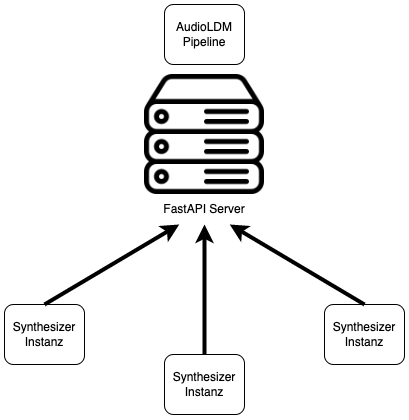
\includegraphics[width=.4\textwidth]{graphics/Server.png}
  \caption[AudiLDM Anbindung]{Anbindung an den \emph{AudioLDM}-Server}
  \label{fig:server}
\end{figure}

\subsection{Sampler}

Für die Implementierung des Samplers wurde der von \emph{Juce} bereitgestellten Sampler \cite{noauthor_sampler_nodate} verwendet. Darüber hinaus wurde die Funktionalität erweitert, um gezielte Tonverschiebungen durchzuführen und den Pitch-Bender eines Keyboards zu verwenden.

\section{Verteilung und Bündelung}

Für \emph{macOS} konnten eine \emph{.app}-Applikationsdatei, eine \emph{VST3}- sowie eine \emph{AU}-Datei generiert werden. Um die Installation der Dateien für den Nutzer zu vereinfachen, wurden diese in eine \emph{pkg}-Installationsdatei gebündelt. 

Der \emph{FastAPI}-Server wurde mittels \emph{pyinstaller} \cite{noauthor_pyinstaller_nodate} zu einer Applikation kompiliert, die der Nutzer unkompliziert öffnen kann. \emph{pyinstaller} integriert alle erforderlichen Abhängigkeiten in einem Paket, sodass der Benutzer die Applikation ausführen kann, ohne einen Python-Interpreter oder sonstige Module installieren zu müssen \cite{noauthor_pyinstaller_nodate}. Da jedoch alle benötigten Module inkludiert werden, resultiert aus einem ursprünglich $5$ KB großen Skript eine Dateigröße von $450$ MB. Die Vergrößerung des Speicheraufwandes ist somit erheblich, jedoch unabdingbar, um den Server und damit ein benutzbares Instrument zu verteilen und zu veröffentlichen. Falls die generierten Server-Applikationen, jedoch auf einem System instabile Performance oder Probleme aufweisen, lässt sich auch das Server-Skript in einer festgelegten \emph{Conda}-Umgebung ausführen. 

Das digitale Instrument wurde sowohl unter \emph{macOS} mit \emph{Silicon}- als auch \emph{Intel}-Chips getestet. Bei der Nutzung der Server-\emph{Applikation} auf Intel-Macs wurde mit zwingendem \emph{torch}-Gerät \emph{cpu} eine mangelhafte und instabile Performance festgestellt. Hierbei empfiehlt sich das Script für den Server, in einer \emph{Cuda}-Umgebung mit den vorgegebenen \emph{Python}-Modulen laufen zu lassen (siehe Kapitel \ref{chap:git})

\section{Benutzeroberfläche}

\begin{figure}[h]
  \centering
  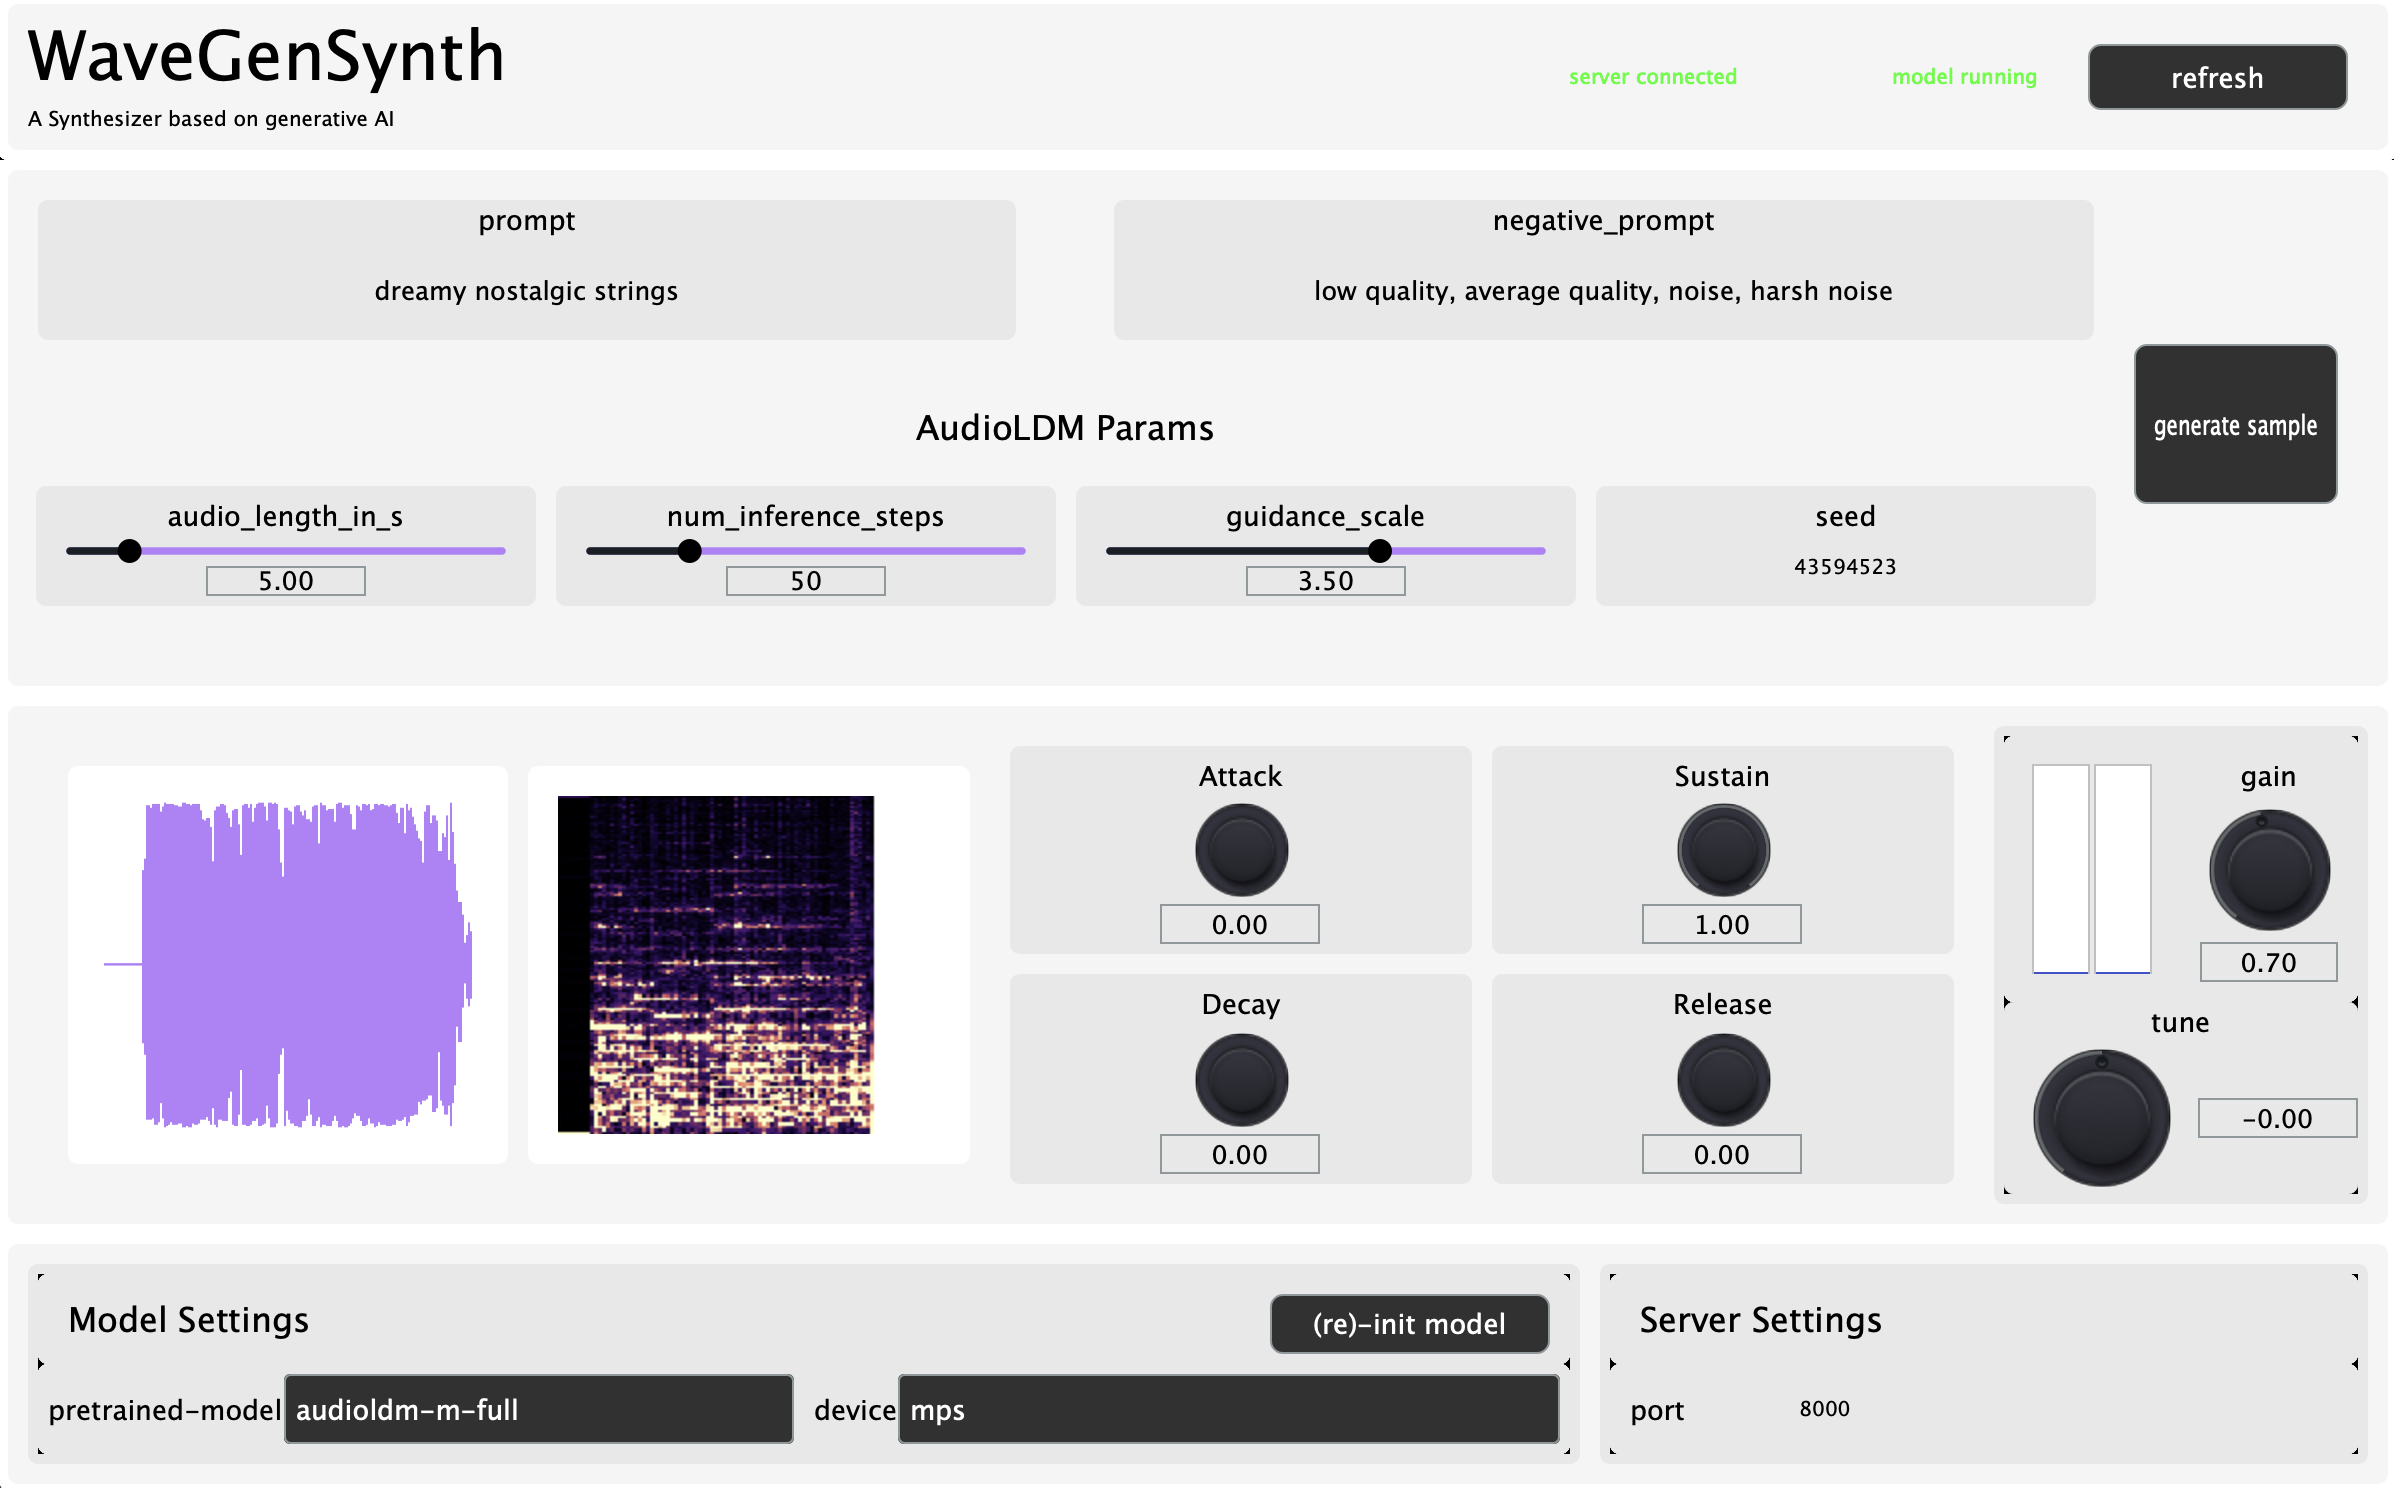
\includegraphics[width=1.0\textwidth]{synth.png}
  \caption[Benutzeroberfläche]{Entstandene Benutzeroberfläche}
  \label{fig:synth}
\end{figure} 

Die resultierende Benutzeroberfläche (Abbildung \ref{fig:synth}) erlaubt es einem Nutzer, eine Verbindung mit der API (siehe \ref{sec:api}) auf einem gewählten Port herzustellen und ein Modell zu initiieren, indem aus einer Palette von vortrainierten Modellen ausgewählt wird. Die Nutzung des Modells auf diversen Hardwarekonfigurationen (mit und ohne GPU) sowie Betriebssystemen wird durch die Auswahl an unterstützten Geräten ermöglicht. Nach der Initialisierung eines Modells kann ein gewünschter Klang, der durch die Texteingabefelder \emph{Prompt} und \emph{Negative Prompt} spezifiziert wird, synthetisiert werden. Zudem lassen sich die Länge des zu erzeugenden Klangs in Sekunden (\emph{audio length}), die Anzahl der Inferenzschritte (\emph{number of inference steps}) und die Leitskala (\emph{guidance scale}) anpassen. Um die Erzeugung deterministisch zu gestalten, kann ein \emph{Seed} in Form eines 8-Byte großen Integers im Wertebereich von $0$ bis $2^{64}-1$ angegeben werden.

Die \emph{Hüllkurve} des \emph{Samplers} (siehe \ref{sec:synth+envelope}) kann über vier Parameter angepasst werden. Hierbei lassen sich die Zeitspannen in Sekunden für die Anschwell- (engl. \emph{attack}), Abschwell- (engl. \emph{decay}) und Ausschwingphasen (engl. \emph{release}) sowie das Niveau, auf das die Lautstärke absinken soll (engl. \emph{sustain}), festlegen. Der von dem Instrument generierte Klang kann durch den Schieberegler "Verstärkung" (engl. \emph{gain}) auf eine spezifische Lautstärke justiert werden.

Da die \emph{Tonhöhe} des generierten Klangs nicht im Voraus festgelegt werden kann und der Klang standardmäßig der \emph{Midi}-Note $C4$ zugeordnet wird, bietet sich die Option, das Instrument mittels des Reglers \emph{tune} so zu stimmen, dass die \emph{Tonhöhe} des Klangs der gespielten Note entspricht. Hierbei lässt sich der Klang kontinuierlich um bis zu zwölf Halbtöne, also einer Oktave, nach oben oder unten modifizieren.

Mithilfe eines \emph{MIDI}-Eingabegeräts lassen sich die verschiedene \emph{Tonhöhen} spielen. Das an vielen Keyboards vorhanden \emph{Pitch-Bend}-Rad, welches eine kontinuierliche \emph{Modulation} des aktuell gespielten Tones um bis zu 2 Halbtöne ermöglicht, kann ebenso von dem Instrument verarbeitet werden. 

Das erzeugte Signal wird mittels einer Wellenform- und Spektrogramm-Anzeige visualisiert. Dies zielt darauf ab, dem Nutzer ein besseres Verständnis der Modellergebnisse zu ermöglichen und das erfolgreiche Generieren zu erkennen. Zudem ermöglicht diese Visualisierung die Identifikation bestimmter Klangstrukturen.


\section{Evaluation}

Eine Darstellung des Verhaltens verschiedener Modelle in Reaktion auf spezifische Parameter und Eingaben ist unter \url{https://suckrowpierre.github.io/TtPS.github.io/} \cite{pierre-louis_suckrow_text-zu-spielbarem-klang_nodate} visualisiert ermöglicht eine einfache Evaluierung dieser. Es ist zu beachten, dass diese Zusammenstellung einen Einblick und einen ersten Eindruck in die Nutzbarkeit der verfügbaren Modelle in Kombination verschiedener Parameter und \emph{Prompts} bieten soll. Aufgrund der begrenzten Anzahl an Beispielen und dem Fehlen einer Studie können jedoch keine definitiven Aussagen über Qualität der Modelle getroffen werden. Die Untersuchungen der Modelle und daraus folgende Ergebnisse beziehen sich auf subjektive empfundene Beobachtungen und Eindrücke.  

Die in \url{https://suckrowpierre.github.io/TtPS.github.io/} \cite{pierre-louis_suckrow_text-zu-spielbarem-klang_nodate} dargestellten Ergebnisse wurden mittels des auf \url{https://github.com/suckrowPierre/ThesisModelsResultsGenerator/} veröffentlichten Codes generiert.

Ergebnisse, bei denen die \emph{torch}-Geräte \emph{mps} und \emph{cpu} zum Einsatz kamen, wurden auf einem \emph{Macbook Pro} mit einem \emph{Apple M1 Pro}-Chip unter \emph{macOS Ventura 13.2.1} erzeugt. Ergebnisse, die mithilfe von Cuda erzeugt wurden, entstanden in einem \emph{Google-Colab} unter Verwendung einer \emph{T4 GPU}.

Die verwendeten \emph{Prompts} wurden unter anderem durch \emph{GPT-4} \cite{openai_gpt-4_2023} auf \url{https://chat.openai.com/} mittels des folgenden \emph{Prompts} (siehe \ref{lst:prompt}) am 8. September 2023 generiert.

\lstdefinestyle{gpt}{
    basicstyle=\ttfamily\small,
    breaklines=true
}
\begin{Listing}
\begin{lstlisting}[style=gpt]
For a scientific work of mine, I'm evaluating the music abilities of diffusion models that can generate audio. For that, I have a script that generates audio for different models based on a list of prompts. My list looks like the following. Please add more prompts to test the musical and instrumental abilities of the models. Keep in mind the people using the models would be musicians, studio engineers, and music producers. 


A single kickdrum
A kickdrum
A distored kickdrum
A kickdrum with a lot of reverb
A clap
A weird clap
A snare
A string orchestra
A analog synth
A distorted analog synth
A string synth
dreamy nostalgic strings
Ambient pads
A guitar string
A distorted guitar string
\end{lstlisting}
    \caption{Benutzer \emph{GPT-4} \emph{Prompt}}
  \label{lst:prompt}
\end{Listing}

\chapter{Ergebnisse}
Die Integration der erörterten Komponenten und Elemente resultierte in einem digitalen Instrument mit den Namen \emph{WaveGenSynth}, das entweder als eigenständige Anwendung oder als Erweiterung in den Formaten VST3 oder AU innerhalb einer Digital Audio Workstation (DAW) wie \emph{Ableton} \cite{noauthor_ableton_nodate} oder \emph{Logic} \cite{noauthor_logic_nodate} verwendet werden kann. Das digitale Instrument ist unter \emph{Github} \cite{noauthor_github_nodate} veröffentlicht \footnote{\url{https://github.com/suckrowPierre/WaveGenSynth}} (siehe \ref{chap:git}). 

Die Soundqualität des Instrumentes und die Fähigkeit die gewünschten musikalischen Merkmale aus der textuellen Eingabe zu generieren hängt von dem zur Verwendung kommenden Modell, und der Nutzer spezifischen Eingabe der Parameter und des \emph{Promptes} ab. 

Es lässt sich feststellen, dass bei gleichen Parametern und \emph{Prompt} für unterschiedliche \emph{Torch}-Geräte diverse Audiosignale erzeugt werden. Ein großer Unterschied in der Qualität zwischen den Geräten lässt sich anhand der $6$ verwendeten \emph{Prompts} nicht eindeutig ermitteln, jedoch zeigt sich eine Tendenz, dass, wenn ein \emph{Prompt} auf den Geräten \glqq\emph{mps}\grqq und \glqq\emph{cuda}\grqq ein schlechtes Ergebnis erzielt, das mittels \glqq\emph{cpu}\grqq generierte Audiosignal für den gleichen \emph{Prompt} noch mehr unerwünschte Artefakte und unangenehme Geräusche aufweist.

Aus \cite{noauthor_huggingface-audioldm_nodate, noauthor_huggingface-audioldm2_nodate} geht der erwartete Einfluss des Werts der \emph{Leitskala} (engl. \emph{guidance-scale}) auf die Signalqualität hervor. Obwohl höhere Werte den beschriebenen \emph{Prompt} präziser abbilden, führen sie zu einer verminderten Audioqualität. Zur Untersuchung dieses Sachverhalts wurden Audiosignale der \emph{Prompts} (\glqq Gentle guitar strum, Tribal African drum circle, vocal harmonies\grqq) mittels sämtlicher verfügbarer vortrainierter Modelle und \emph{Leitskala}-Werten von $1,2,3,4,5$ generiert. Es zeigt sich, dass Audiosignale, die mit einem Wert von $1$ erzeugt wurden, die niedrigste Qualität aufweisen. Werte zwischen $2-4$ scheinen hingegen eine bessere Audioqualität zu gewährleisten. Die bedeutenden Audiocharakteristika scheinen sich in diesem Bereich zu kristallisieren, und tiefe \emph{Frequenzen} treten in Erscheinung. Weiterhin bestätigt sich, dass höhere Werte den gegebenen \emph{Prompt} detaillierter repräsentieren. Ein exemplarischer Fall hierfür ist der \emph{Prompt} \glqq Gentle guitar strum\grqq, generiert mit \emph{audioldm-m-full} \cite{noauthor_cvsspaudioldm-m-full_nodate}. Bei diesem zeigen Signale mit einem Wert unter $4$ diverse Audioereignisse, die an eine Gitarre erinnern. Erst bei einem Wert von $4$ oder höher ist ein einzelnes, eindeutiges Gitarrenzupfen zu identifizieren.

Die \emph{Inferenzschritte} (engl. \emph{Inferencesteps}) geben die Anzahl der Entrauschungsschritte im \emph{Diffusions}-prozess an. Eine höhere Anzahl dieser Schritte soll zu verbesserten Ergebnissen bei gleichzeitig längerer Inferenzzeit führen \cite{noauthor_huggingface-audioldm2_nodate, noauthor_huggingface-audioldm_nodate}. Um die Auswirkungen der \emph{Inferenzschritte} zu analysieren, wurden wieder Audiosignale aus drei unterschiedlichen \emph{Prompts} (\glqq ambient texture\grqq, \glqq techno kickdrum\grqq, \glqq Long evolving drone\grqq) mithilfe aller vorab trainierten Modelle und für Inferenzschritte-Anzahlen von $5,10,20,50,100,200,400$ generiert. Hierbei zeigten die Werte $5$ und $400$ die ungünstigsten Ergebnisse: Signale mit $5$ Schritten resultierten in dumpfen und wenig strukturierten Klängen. Hingegen schienen Werte im Bereich von $10-200$ adäquate Resultate zu liefern. Es wurden oftmals nur marginale Qualitätsveränderungen pro Schritt beobachtet. Die Ergebnisse weisen zudem darauf hin, dass \emph{AudioLDM2} im Vergleich zu \emph{AudioLDM} eine größere Anzahl an Schritten benötigt, um qualitativ hochwertige Signale zu produzieren. Bei $400$ Schritten hingegen erscheint die Anzahl überdimensioniert, da das resultierende Signal verstärkt abstrakte Klangereignisse und unerwünschte Artefakte aufweist.

Um die Auswirkungen der gewünschten Audiosignallänge auf die Resultate zu untersuchen, wurden für die drei \emph{Prompts} (\glqq Chirping birds at dawn\grqq, \glqq A choir pad\grqq, \glqq An ambient electronic pad\grqq) mittels der Modelle \emph{audioldm-m-full} \cite{noauthor_cvsspaudioldm-m-full_nodate} und \emph{audioldm2} \cite{noauthor_cvsspaudioldm2_nodate} Signale mit den Längen $5,10,20,30$ generiert. Bei ausgedehnteren Signalen scheint die Qualität leicht abzunehmen. Offenbar haben die Modelle Schwierigkeiten, die Konsistenz über längere Zeiträume hinweg beizubehalten. In einigen dieser Beispiele manifestiert sich ein Phänomen, das als \emph{Pitchdrifting} bezeichnet wird, wodurch die wahrgenommene Tonhöhe variiert. Diese leicht reduzierte Qualität könnte jedoch gezielt als stilistisches Mittel verwendet werden.

Die Einwirkung verschiedener \emph{Negative-Prompts} (engl. \emph{negative prompt}) auf die \emph{Prompts} (\glqq Soft flute note\grqq, \glqq Choir\grqq, \glqq A muted trumpet\grqq) wurde analysiert. Mittels der Modelle \emph{audioldm-m-full} \cite{noauthor_cvsspaudioldm-m-full_nodate} und \emph{audioldm2-music} \cite{noauthor_cvsspaudioldm2-music_nodate} wurden Signale unter Verwendung der \emph{Negativen Prompts} (\glqq low quality\grqq, \glqq average quality\grqq, \glqq harsh noise\grqq, \glqq dissonant chords\grqq, \glqq distorted sounds\grqq, \glqq clashing frequencies\grqq, \glqq feedback loop\grqq, \glqq clattering\grqq, \glqq inharmonious\grqq, \glqq noise\grqq, \glqq high pitch\grqq, \glqq artefacts\grqq) generiert. Die Beobachtungen zeigen, dass einige \emph{Negative-Prompts} das Ergebnis positiv beeinflussen, während andere das Signal mit zusätzlichem Rauschen beeinträchtigen. Insbesondere \glqq low quality\grqq, \glqq noise\grqq, \glqq harsh noise\grqq und \glqq average quality\grqq schienen das Resultat am meisten zu verbessern. Der \emph{Negative-Prompt} \glqq distorted sounds\grqq zeigte in einigen Fällen positive Effekte, bewirkte jedoch im Zusammenhang mit dem \emph{Prompt} \glqq Soft flute note\grqq und dem Modell \emph{audioldm-m-full} eine Verschlechterung. \glqq high pitch\grqq scheint hohe \emph{Obertöne} zu unterdrücken und tiefere Töne bekommen mehr Präsenz, was eine bewusste Entscheidung seien sollte. Andere \emph{Negative-Prompts}, wie \glqq dissonant chords\grqq, \glqq distorted sounds\grqq, \glqq clashing frequencies\grqq, \glqq feedback loop\grqq, \glqq clattering\grqq, \glqq inharmonious\grqq und \glqq artefacts\grqq, scheinen das Resultat zu beeinträchtigen. Die anfängliche Annahme, dass \emph{AudioLDM2} aufgrund von \emph{LOLA} effizienter mit \emph{Negative-Prompts} interagieren könnte, wurde durch die ungünstigen Ergebnisse von \emph{audioldm2-music} in den gegebenen Tests nicht bestätigt.

Erwartungen, dass \emph{Prompts} wie \glqq A kickdrum\grqq, \glqq A snare\grqq, \glqq Loud clap sound\grqq, \glqq A gong hit\grqq \, ein singuläres, nicht wiederholendes Audioereignis erzeugen, werden nicht erfüllt. In den meisten Fällen produzieren die Modelle Signale, in denen Audioereignisse mehrfach auftreten. Die Modelle scheinen nicht darauf ab zu zielen, das gewünschte einzelne Ereignis zu synthetisieren, sondern generieren das angestrebte Ergebnis in einem musikalischen Rhythmus. Eine präzise Formulierung, die ausschließlich ein einzelnes Audioereignis und einen Ton erwartet – ausgedrückt durch \glqq A single\grqq –, scheint bei \emph{audioldm2} \cite{noauthor_cvsspaudioldm2_nodate} effektiver zu sein. Im Gegensatz dazu zeigt \emph{audioldm2-music} \cite{noauthor_cvsspaudioldm2-music_nodate} auch mit dieser Formulierung keine verbesserten Ergebnisse. Es wird vermutet, dass \emph{audioldm2-music} \cite{noauthor_cvsspaudioldm2-music_nodate} dazu neigt, wiederholende Strukturen zu generieren, da sein Hauptziel die Generierung musikalischer Ergebnisse und nicht eines isolierten Klangs ist.

Der Versuch, instrumententypische Klänge durch die \emph{Prompts} \glqq FM synthesis bells\grqq, \glqq mellotron chords\grqq, \glqq A bagpipe melody\grqq, \glqq A guitar string\grqq und \glqq A piano chord\grqq zu generieren, brachte nicht die gewünschten Ergebnisse. Die erzeugten Signale klingen abstrakt und stellen keine akkurate Audiorepräsentation der jeweiligen Eingabe dar. Zudem ist festzustellen, dass weniger zufriedenstellende Ergebnisse von \emph{AudioLDM2} eine Neigung haben, ähnliche zu klingen.

Das Schmücken des \emph{Prompts} mit Emotionen und zusätzlichen Beschreibungen, wie beispielsweise \glqq Dark pad sound\grqq, \glqq An ethereal shimmering synth pad\grqq, \glqq An angelic choir\grqq, \glqq dreamy nostalgic strings\grqq und \glqq a sad violin solo\grqq, scheint die generierten Signale interessanter zu gestalten. Dies ermöglicht den Anwendern, den zu erzeugenden Klang stärker in eine bestimmte Richtung zu beeinflussen. Hierbei wurde wieder beobachtet, dass die Ergebnisse von \emph{AudioLDM2} trotz variierender \emph{Prompts} eine Tendenz zu ähnlichen Klangstrukturen zeigen.

Die Modelle scheinen auf bestimmte Beschreibungen musikalischer und akustischer Effekte adäquat reagieren zu können. Das langanhaltende Ausklingen eines Tones, umschrieben durch den Ausdruck \glqq long sustain\grqq, funktioniert offenbar zufriedenstellend. Ebenso scheint das Hinzufügen von Hall durch \glqq reverb\grqq, Verzerrung mittels \emph{distortion} und das Umkehren eines Tones durch \glqq reverse\grqq gut zu funktionieren. Komplexere Effekte wie Echo (\glqq echo\grqq), Verstimmung (\glqq detune\grqq) und Verzögerung (\glqq delay\grqq) können gelegentlich zu den gewünschten Ergebnissen führen. Interessanterweise scheinen die \emph{AudioLDM}-Modelle in diesem Aspekt besser abzuschneiden als die \emph{AudioLDM2}-Modelle, obwohl man aufgrund der \emph{LOA}-Repräsentation erwarten könnte, dass letztere bessere Ergebnisse erzielen könnten.

Bei dem Versuch, \emph{Prompts} mit spezifischen, in der Musikproduktion oder der Pop-Kultur häufig verwendeten Klängen und Begriffen zu definieren scheiterte. Die Bemühungen, eine im Hip-Hop häufig verwendete \emph{808-Kickdrum} oder eine in der elektronischen Musik verwendete \emph{909-Kickdrum} zu erzeugen, lieferten Ergebnisse, deren \emph{Klangfarbe} nicht den Vorgaben entsprach. Auch der Versuch, einen \emph{Amen-Break}, das wohl am meisten verwendete \emph{Sample} weltweit, zu erzeugen, brachte nicht das gewünschte Ergebnis. Eine Ähnlichkeit mit einer \emph{303 Baseline} konnte lediglich durch \emph{audioldm-m-full} erreicht werden, während die anderen Modelle scheiterten. Die \emph{Prompts} \glqq A Juno-106 pad\grqq{} und \glqq Oberheimer OB-Xa string pads\grqq{} erzeugten verwendbare \emph{Pads}, also lange gehaltene Töne oder Akkorde. Es lässt sich jedoch streiten, ob sie die klanglichen Feinheiten dieser Instrumente besitzen. 

\chapter{Diskussion}
Das Aufzeigen, der Möglichkeit Instrumente basierend auf künstlicher Intelligenz zu entwickeln, stellt eine bedeutende Erweiterung in der musikalischen Klangerzeugung dar. Die Analyse des digitalen Instruments und die Bewertung der anwendbaren Modelle deuten darauf hin, dass die Generierung, Manipulation und Reproduktion von Klängen, die durch künstliche Intelligenz synthetisiert wurden, ein hohes kreatives Potential aufweisen. Es treten jedoch bestimmte Einschränkungen und Schwachstellen auf. Zu diesen zählen insbesondere die identifizierten Mängel, das gelegentlich unvorhersehbare Verhalten der Modelle sowie die begrenzte Implementierung des Samplers.

Es zeigt sich, dass die analysierten Modelle bisher nicht angemessen auf Eingabeaufforderungen im Bereich der Musikproduktion reagieren. Die Unfähigkeit einiger Modelle, einzelne Klangereignisse zu generieren, das Fehlen der Modellierung erwarteter Klangmerkmale spezifischer Instrumente sowie das Auftreten verrauschter Ergebnisse weisen auf bestehende Defizite hin. Diese Mängel könnten durch das Training mit umfangreicheren Audiodaten, die in der Musikproduktion eingesetzt werden, adressiert werden. Potenzielle Quellen für solche Trainingsdaten sind Synthesizer- oder Samplermanufakturen, Audiobibliotheken wie \emph{Splice} \cite{noauthor_royalty-free_nodate}, Musikstudios oder auch Produzenten selbst. Privatpersonen, die sich mit Musikproduktion beschäftigen, verfügen häufig über eigene Klangbibliotheken, die in ihren Werken Anwendung finden. Auf Basis dieser Daten könnte ein Modell weiter verfeinert werden, um es individueller und persönlicher zu gestalten. Eine solche Personalisierung von \emph{AudioLDM} \cite{liu_audioldm_2023} wurde in \cite{plitsis_investigating_2023} untersucht und könnte in \emph{generative AI}-Werkzeuge für Musikproduzenten integriert werden. Eine weitere Überlegung wäre, die Klangbibliotheken verschiedener Privatpersonen zu einer umfangreichen Datenbasis zusammenzuführen, die anschließend für das Finetuning oder Training verwendet werden könnte. Ein solcher, von der Community getriebener Ansatz, könnte ein demokratisches Mittel darstellen, um den Mangel an Datensätzen in diesem Bereich zu beheben. 

Benutzte Modelle sollten darauf abzielen, Ergebnisse mit der von der \emph{Audio Engineering Society} empfohlenen \emph{Sampling}-Rate von $48$kHz \cite{audio_engineering_society_inc_aes5-2018_2018} zu erzeugen. Die Modelle \emph{AudioLDM} \cite{liu_audioldm_2023} und \emph{AudioLDM2} \cite{liu_audioldm2_2023} produzieren Ergebnisse mit einer Rate von $16$kHz und sind daher nicht geeignet, um Klänge in \emph{High Fidelity} zu generieren. Eine kürzere \emph{Inferenzzeit} könnte die \emph{User-Experience} des Instruments positiv beeinflussen.

Es ist wünschenswert, dass eingesetzte Modelle Ergebnisse mit der von der \emph{Audio Engineering Society} empfohlenen \emph{Sampling}-Rate von $48$kHz \cite{audio_engineering_society_inc_aes5-2018_2018} liefern. Die Modelle \emph{AudioLDM} \cite{liu_audioldm_2023} und \emph{AudioLDM2} \cite{liu_audioldm2_2023} generieren Ergebnisse mit einer Rate von $16$kHz und sind daher für die Generierung von Klängen in \emph{High Fidelity} nicht optimal. Eine verkürzte \emph{Inferenzzeit} könnte zudem die \emph{User-Experience} des Instruments verbessern.

Das Scheitern der Erstellung einer ONNX- bzw. TorchScript-Repräsentation des Modells für die Inferenz in C++ führt zu Komplikationen bei der Bündelung und Verteilung des Modells in Verbindung mit der Python API. Durch die Erstellung einer solchen \emph{binären} Datei für das verwendete Modell würde die Notwendigkeit eines Servers und einer API entfallen. Ebenso wäre der Einsatz mehrerer Programmiersprachen für eine Implementierung nicht länger erforderlich.

Die rudimentäre Implementierung des Samplers ermöglicht nicht die Definition von Start- und Endpunkten für die Wiedergabe des generierten Signals. Solche Parameter könnten eine intuitive Möglichkeit bieten, das gewünschte Klangereignis aus mehreren oder wiederholten Ereignissen auszuwählen. Zudem fehlt die Möglichkeit, spezifische Klangsegmente zu wiederholen, um einen durchgängigen Klang zu erzeugen – eine Funktion, die in industriellen Samplern seit den 1990er Jahren üblich ist. Vor diesem Hintergrund stellt sich die Frage nach der Notwendigkeit, einen eigenen Sampler zu entwickeln. Alternativ könnte eine Benutzeroberfläche ausreichen, die sich in bestehende Musikproduktionssoftware integrieren lässt, um Klänge zu generieren und mittels der Werkzeuge des jeweiligen Software-Ökosystems zu manipulieren. Eine solches Anwendung könnte, vorausgesetzt das Modell ist leistungsstark genug, Anwendungen wie \emph{Splice} \cite{noauthor_royalty-free_nodate} überflüssig machen. Die in \emph{AudioLDM} \cite{liu_audioldm_2023} präsentierten Generierungsfunktionen, wie Inpainting oder Style-Transfer, könnten in einem solchen Werkzeug integriert werden. Dies würde Nutzern beispielsweise erlauben, unerwünschte Abschnitte eines Spektrogramms zu eliminieren oder Audiodateien zu importieren und durch Eingabeaufforderungen zu verändern.

Sollte die Entwicklung eines speziell angefertigten Samplers fortgesetzt werden, könnten diesem auch Elemente des maschinellen Lernens hinzugefügt werden. Beim Spielen unterschiedlicher Noten auf einem Klavier erzeugen diese verschiedene \emph{Klangfarben} und folglich unterschiedliche Spektren \cite{parker_good_2009}. Es genügt nicht, den Klang lediglich auf die gewünschte \emph{Frequenz} zu modulieren. Um ein realistischeres Ergebnis zu erzielen, müssen die feinen Unterschiede der Oberschwingungen für jede \emph{Tonhöhe} angepasst werden. Ein solches Anpassungsverfahren könnte durch ein ML-Modell erlernt werden. Als Eingabe würde ein Audiosignal dienen, aus welchem das Modell Signale für alle möglichen \emph{Tonhöhe} generiert. Für das Training eines solchen Modells wäre eine umfangreiche Sammlung von Audiosignalen erforderlich, die alle \emph{Tonhöhe} verschiedener Instrumente abdecken.

Einige Musiker bevorzugen es, sich von Computern zu distanzieren und spezialisierte Hardware zu nutzen, die ein haptischeres Feedback bietet. Die in dieser Arbeit präsentierte spielbare Klangsynthese könnte auf ein dediziertes Hardware-Gerät übertragen werden. Lösungen für \emph{Deep Learning} auf Microcontrollern \cite{saha_machine_2022} können auf dedizierten Hardware-Plattformen, wie den \emph{Coral}-Geräten \cite{noauthor_coral_nodate} von Google oder den \emph{Jetson}-Geräten \cite{noauthor_jetson_nodate} von Nvidia, betrieben werden. Der Code für das Instrument müsste dann lediglich für eine bestimmte Hardware entwickelt und gewartet werden. Dies würde für Musiker, die keine Kenntnisse in \emph{Python} oder \emph{C++} besitzen, den Vorteil bieten, dass sie sich nicht mit der Installation und Betreiben der Software auseinandersetzen müssen. Einige Microcontroller-Lösungen, wie \emph{Coral}, erfordern jedoch, dass das verwendete Modell mit \emph{TensorFlow Lite} \cite{noauthor_tensorflow_nodate} kompatibel ist. Hierbei stellt sich wieder die Frage, ob umfangreiche und komplexe Modelle, wie \emph{AudioLDM} \cite{liu_audioldm_2023} und \emph{AudioLDM2} \cite{liu_audioldm2_2023}, in dieses Format konvertiert werden können.

Weitere Mängel des Instruments, die adressiert und optimiert werden könnten, betreffen beispielsweise das manuelle Stimmen, welches sich automatisierten ließ. Ein weiteres Defizit besteht darin, dass die bisher generierten Klänge und Einstellungen sich nicht, wie bei vielen digitalen Instrumenten üblich, speichern und wieder abrufen lassen. Für die Erstellung dieses ersten Prototyps wurde auf die \emph{Spezifikation und Verifikation} des \emph{Quellcodes} verzichtet. Bei einer Weiterverfolgung der Implementierung sollte dieser Aspekt jedoch berücksichtigt werden, um potenzielle \emph{Bugs} und Fehler im Code zu minimieren.

Ungeachtet der genannten Defizite und Schwachstellen hat sich gezeigt, dass das digitale Instrument mithilfe der vorgestellten \emph{Diffusions}-Modelle in der Lage ist, spielbare und manipulierbare Klänge aus benutzerspezifischen Eingaben zu generieren. Weiterhin wurde bestätigt, dass das Instrument in moderne Musikproduktionsprozesse und die damit verbundenen Anwendungen integriert werden kann. Es erschließt eine neue Form der Soundsynthese durch künstliche Intelligenz und bietet somit innovative Möglichkeiten, Klanglandschaften zu gestalten. Ein wesentlicher Vorteil gegenüber der Generierung anderer Medien besteht darin, dass auch unerwartete oder minderwertige Ergebnisse weiterverwendet werden können, indem sie durch diverse Effekte und Prozesse umfassend bearbeitet und transformiert werden. Ein Beispiel hierfür liefert der Musiker \glqq Heinbach\grqq, der in \cite{hainbach_how_2021} erläutert, wie er den von \glqq Bob Ross\grqq geprägten Begriff \emph{Happy Little Accidents} in den Musikbereich überträgt und unerwartete Klänge musikalisch aufarbeitet, um neue \emph{Klangfarben} und -landschaften zu schaffen. Zusammenfassend lässt sich feststellen, dass das entwickelte Instrument in seiner aktuellen Form mit den verfügbaren generativen Modellen weniger zur qualitativ hochwertigen Modellierung spezifischer Klänge geeignet ist, sondern vielmehr zum Experimentieren mit neuen, unerwarteten Klängen verlockt.

\chapter{Schlussfolgerung}
Diese Arbeit zielte darauf ab, musikalische Konzepte, elektronischer Klangerzeugung, digitaler Audiorepräsentation, \emph{generative AI} mittels \emph{Latenter Diffusion} und Softwareframeworks zu verknüpfen. Es wurde erfolgreich ein digitales Instrument entwickelt, das die Erzeugung innovativer, spielbarer und manipulierbarer Klangergebnisse ermöglicht. Dies unterstreicht die Machbarkeit eines solchen Unterfangens, auch wenn es bestimmten Einschränkungen und Defiziten erfasst wurden.

Die Komplexität der verwendeten Modelle \emph{AudioLDM} \cite{liu_audioldm_2023} und \emph{AudioLDM2} \cite{liu_audioldm2_2023} ließ eine erfolgreiche Konvertierung in eine binäre Repräsentation scheitern und beschränkte dadurch die möglichen Implementierungsmethoden. Es wurde sich für die Implementierung des Instruments über eine lokal gehostete \emph{API} entschieden, die die vortrainierten Modelle \emph{AudioLDM} und \emph{AudioLDM2} initialisieren und mit diesen Inferenz betreiben kann. Dieser Ansatz führte allerdings zu einer erhöhten Komplexität bei der Bündelung und Verteilung des Instruments, wodurch zwei separate ausführbare Applikationen entstanden.

Die Auswertung der Qualität der Ergebnisse von \emph{AudioLDM} \cite{liu_audioldm_2023} und \emph{AudioLDM2} \cite{liu_audioldm2_2023} im Hinblick auf die erwarteten \emph{Prompts} im Kontext der Nutzung des digitalen Instruments offenbarte Limitierungen. Diese Einschränkungen begrenzen die Anwendbarkeit des Instruments primär auf die Exploration neuer teils unerwarteter Klänge. Dennoch, trotz dieser Limitierungen liegt hierin das Potenzial, diese unvorhergesehenen und vielleicht befremdlichen Klänge als Basis für weitere Manipulationen und Umformung zu nutzen. Zukünftig könnten verbesserte und weiterentwickelte Modelle bei gesteigerter Klangqualität und reduzierten Artefakten im Klang konventionellen Instrumenten gleich kommen. Das Potenzial eines individuellen \emph{finetuning} durch eigene Klangbibliotheken wurde erkannt und auf eine Verbesserung der \emph{Abtastrate} auf $48$kHz hingewiesen. 

Die Abwesenheit von Funktionen, die es erlauben, Start- und Endpunkte der wiedergegebenen Töne anzupassen sowie Loop-Points zu definieren, für ein kontinuierliches Anhalten eines Klanges, limitiert die Bearbeitungsmöglichkeiten des generierten Klanges. Zudem würde das Instrument von zusätzlichen Optimierungen wie einer automatischen Stimmfunktion und der Möglichkeit, Klänge zu speichern und abzurufen, profitieren.

Trotz dieser Mängel ist es unbestreitbar, dass die Arbeit das Potenzial der musikalischen Anwendung von \emph{Diffusions}-Modellen unterstreicht, und eine verbesserte und vielseitigere Integrationsmöglichkeit in moderne Musikproduktionsökosysteme im Vergleich zu ähnlichen Anwendungen bietet. Anwender können Klänge nach ihren Vorstellungen parametrisieren und erzeugen, das Klangverhalten dieser beim Spielen durch eine \emph{Envelope} modifizieren, das Instrument stimmen und die Lautstärke justieren. Eingabegeräte können mittels \emph{MIDI} angeschlossen und das \emph{Pitch-Bend}-Rad kann ebenso verwendet werden.

Es ist zu hoffen, dass zukünftige Forschungen in diesem Bereich von den in dieser Arbeit gemachten Entdeckungen profitieren und diese weiterführen werden. Perspektiven für weitere diverse potenzielle Integration generativer Künstlicher Intelligenz in den Ablauf der Musikproduktion wurden aufgezeigt. 

\label{sec:conclusion}


\printbibliography

All links were last followed on \today{}.

\appendix
\chapter{Veröffentlichung}
\label{chap:git}
Der auf \emph{GitHub} \cite{noauthor_github_nodate} veröffentlichte Code befindet sich im Repository \url{https://github.com/suckrowPierre/WaveGenSynth}. Die für diese Arbeit relevante Version ist im Branch \glqq thesis\grqq , \url{https://github.com/suckrowPierre/WaveGenSynth/tree/thesis} zu finden. Das Repository umfasst den Quellcode sowohl für das digitale Instrument als auch für den \emph{FastApi}-Server. Zusätzlich sind ein Plugin-Installer für Mac, ausführbare Server-Dateien für die Silicon- und Intel-Architekturen auf Mac sowie eine Zip-Datei vorhanden. Letztere beinhaltet das \emph{Python}-Skript für den Server und die benötigten \emph{Python}-Pakete für \emph{Conda}, welche die Ausführung des Servers ohne eine ausführbare Datei ermöglichen.

Die README-Datei bietet Anleitungen zur Installation und Ausführung des Codes.


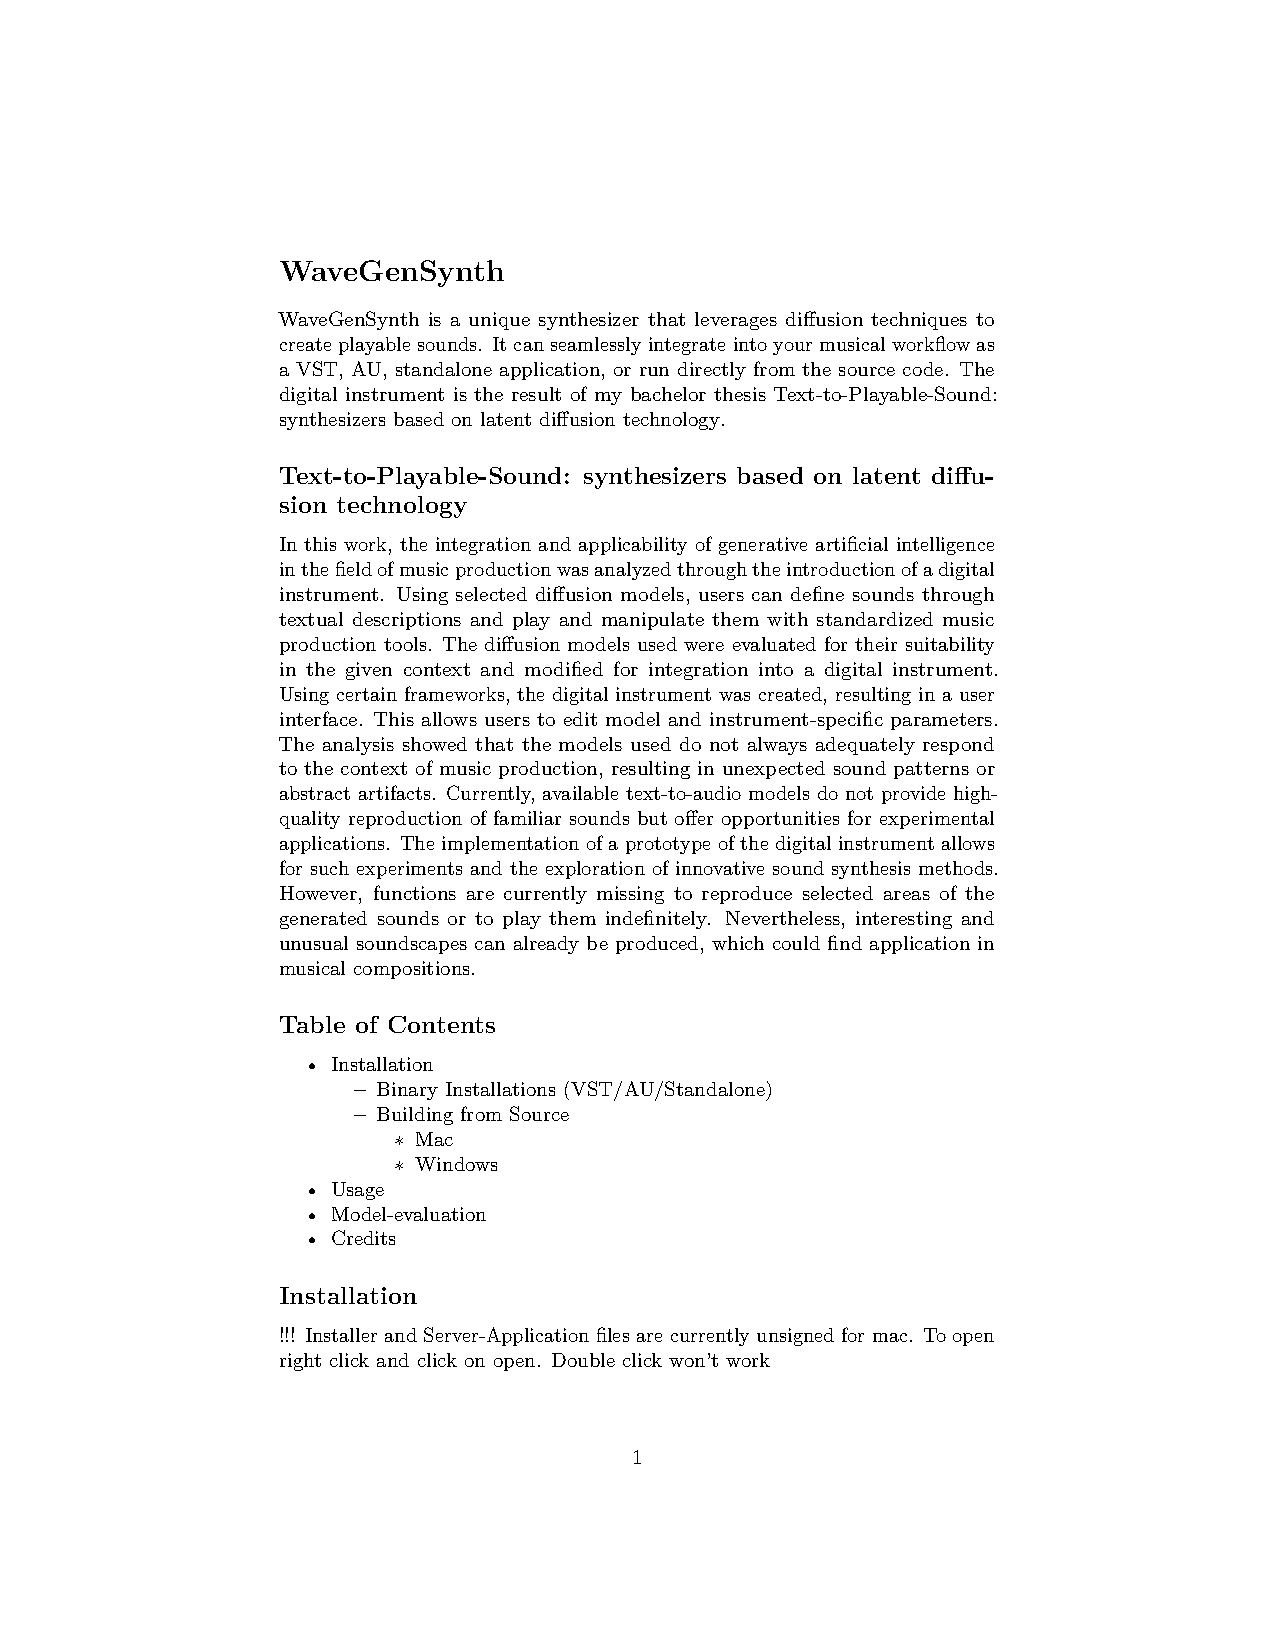
\includepdf[pages=-]{code/README.pdf}


\chapter{Erzeugung der Ergebnisse}
\label{chap:prompts}




%% !TeX root = main-english.tex
% !TeX spellcheck = en-US
% !TeX encoding = utf8
% -*- coding:utf-8 mod:LaTeX -*-

%This smart spell only works if no changes have been made to the chapter 
%using the options proposed in preambel/chapterheads.tex.
\setchapterpreamble[u]{%
  \dictum[Albert Einstein]{We cannot solve our problems with the same level of thinking that created them}
}
\chapter{LaTeX Hints}
\label{chap:latexhints}

One sentence per line.
This rule is important for the usage of version control systems.
A new line is generated with a blank line.
As you would do in Word:
New paragraphs are generated by pressing enter.
In LaTeX, this does not lead to a new paragraph as LaTeX joins subsequent lines.
In case you want a new paragraph, just press enter twice (!).
This leads to an empty line.
In word, there is the functionality to press shift and enter.
This leads to a hard line break.
The text starts at the beginning of a new line.
In LaTeX, you can do that by using two backslashes (\textbackslash\textbackslash).
This is rarely used.

Please do \textit{not} use two backslahes for new paragraphs.
For instance, this sentence belongs to the same paragraph, whereas the last one started a new one.
A long motivation for that is provided at \url{http://loopspace.mathforge.org/HowDidIDoThat/TeX/VCS/#section.3}.

One can write \emph{emphasized text (rendered in italics)} and \textbf{bold text}.

\section{File Encoding and Support of Umlauts}
\label{sec:firstsectioninlatexhints}
The template offers foll UTF-8 support.
All recent editors should not have issues with that.

\section{Citations}


References are set by means of \texttt{\textbackslash cite[key]}.

\begin{filecontents*}{\democodefile}
Example: \cite{WSPA} or by author input: \citet{WSPA}.
\end{filecontents*}
\PrintDemo{style=parallel}

The following sentence demonstrates
\begin{inparaenum}[1.]
  \item the capitalization of author names at the beginning of the sentence,
  \item the correct citation using author names and the reference,
  \item that the author names are a hyperlink to the bibliography and that
  \item the bibliography contains the name prefix \qq{van der} of \qq{Wil M.\,P.\ van der Aalst}.
\end{inparaenum}

\begin{filecontents*}{\democodefile}
\Citet{RVvdA2016} present a study on the effectiveness of workflow management systems.
\end{filecontents*}
\PrintDemo{style=parallel}

The following sentence demonstrates that you can overwrite the text part of the generated label using \texttt{label} in a bibliopgrahie"=entry, but the year and the uniqueness is still generated by biber.

\begin{filecontents*}{\democodefile}
The workflow engine Apache ODE \cite{ApacheODE} executes \BPEL processes reliably.
\end{filecontents*}
\PrintDemo{style=parallel}

\begin{filecontents*}{\democodefile}
Words are best enclosed using \texttt{\textbackslash qq\{..\}}, then the correct quotes are used.
\end{filecontents*}
\PrintDemo{style=parallel}

When creating the Bibtex file it is recommended to make sure that the DOI is listed.

\section{Formulas and Equations}
\label{sec:mf}

\begin{filecontents*}{\democodefile}
Equations $f(x)=x$ inside the text can be provided.
\end{filecontents*}
\PrintDemo{style=parallel}

A list with all available mathematical symbols is provided at \url{http://texdoc.net/pkg/symbols-a4}.

\begin{filecontents*}{\democodefile}
As example the set of natural numbers is given by $\mathbb{N}$.
\end{filecontents*}
\PrintDemo{style=parallel}

For the documentation of editing mathematical formulas read the package documentation of \texttt{amsmath}\footnote{\url{http://texdoc.net/pkg/amsmath}}.

Equation~\ref{eq:test} is numbered and can be referenced in the text:
\begin{filecontents*}{\democodefile}
\begin{align}
  \label{eq:test}
  x = y
\end{align}
\end{filecontents*}
\PrintDemo{style=parallel}

Following equation is not numbered because of using \texttt{\textbackslash align*} as environment.
\begin{filecontents*}{\democodefile}
\begin{align*}
  x = y
\end{align*}
\end{filecontents*}
\PrintDemo{style=parallel}

The template offers \verb+\abs+ to enable the bars scaling well at the absolute value:

\begin{filecontents*}{\democodefile}
$\abs{X}$.
\end{filecontents*}
\PrintDemo{style=parallel}

More details about mathematical environments provides the documentation available at \url{http://www.ctan.org/tex-archive/help/Catalogue/entries/voss-mathmode.html}.


%%%%%%%%%%%%%%%%%%%%%%%%%%%%%%%%%%%%%%%%%%%%%%%%%%%%%%%%%%%%%%%%%%%%%%%%%%%%%%
\section{Sourcecode}
%%%%%%%%%%%%%%%%%%%%%%%%%%%%%%%%%%%%%%%%%%%%%%%%%%%%%%%%%%%%%%%%%%%%%%%%%%%%%%
\Cref{lst:ListingANDlstlisting} shows how to emmbed source code.
With \texttt{\textbackslash lstinputlisting} the source code can be loaded directly from files.

%Listing-Umgebung wurde durch \newfloat{Listing} definiert
\begin{Listing}
  \begin{lstlisting}
<listing name="second sample">
  <content>not interesting</content>
</listing>
\end{lstlisting}
  \caption{The code is separated by two horizontal lines in the listings environment.}
  \label{lst:ListingANDlstlisting}
\end{Listing}

\begin{filecontents*}{\democodefile}
Source code is also available in the text \lstinline|<listing />|.
\end{filecontents*}
\PrintDemo{style=parallel}


%%%%%%%%%%%%%%%%%%%%%%%%%%%%%%%%%%%%%%%%%%%%%%%%%%%%%%%%%%%%%%%%%%%%%%%%%%%%%%
\section{Pseudocode}
%%%%%%%%%%%%%%%%%%%%%%%%%%%%%%%%%%%%%%%%%%%%%%%%%%%%%%%%%%%%%%%%%%%%%%%%%%%%%%
\Cref{alg:sample} shows a sample algorithm.
\begin{Algorithmus} %Use the environment only if you want to place the algorithm similar to graphics from TeX
  \caption{Sample algorithm}
  \label{alg:sample}
  \begin{algorithmic}
\Procedure{Sample}{$a$,$v_e$}
\State $\mathsf{parentHandled} \gets (a = \mathsf{process}) \lor \mathsf{visited}(a'), (a',c,a) \in \mathsf{HR}$
\State \Comment $(a',c'a) \in \mathsf{HR}$ denotes that $a'$ is the parent of $a$
\If{$\mathsf{parentHandled}\,\land(\mathcal{L}_\mathit{in}(a)=\emptyset\,\lor\,\forall l \in \mathcal{L}_\mathit{in}(a): \mathsf{visited}(l))$}
\State $\mathsf{visited}(a) \gets \text{true}$
\State $\mathsf{writes}_\circ(a,v_e) \gets
\begin{cases}
\mathsf{joinLinks}(a,v_e) & \abs{\mathcal{L}_\mathit{in}(a)} > 0\\
\mathsf{writes}_\circ(p,v_e)
& \exists p: (p,c,a) \in \mathsf{HR}\\
(\emptyset, \emptyset, \emptyset, false) & \text{otherwise}
\end{cases}
$
\If{$a\in\mathcal{A}_\mathit{basic}$}
  \State \Call{HandleBasicActivity}{$a$,$v_e$}
\ElsIf{$a\in\mathcal{A}_\mathit{flow}$}
  \State \Call{HandleFlow}{$a$,$v_e$}
\ElsIf{$a = \mathsf{process}$} \Comment Directly handle the contained activity
  \State \Call{HandleActivity}{$a'$,$v_e$}, $(a,\bot,a') \in \mathsf{HR}$
  \State $\mathsf{writes}_\bullet(a) \gets \mathsf{writes}_\bullet(a')$
\EndIf
\ForAll{$l \in \mathcal{L}_\mathit{out}(a)$}
  \State \Call{HandleLink}{$l$,$v_e$}
\EndFor
\EndIf
\EndProcedure
  \end{algorithmic}
\end{Algorithmus}

\clearpage
And if you want to write an algorithm that goes over several pages, you can only do this with the following \textbf{dirty} hack:

{
\begin{minipage}{\textwidth}
  \hrule height .8pt width\textwidth
  \vskip.3em%\vskip\abovecaptionskip\relax
  \stepcounter{Algorithmus}
  \addcontentsline{alg}{Algorithmus}{\protect\numberline{\theAlgorithmus}{\ignorespaces Description \relax}}
  \noindent\textbf{Algorithmus \theAlgorithmus} Description
  %\stepcounter{algorithm}
  %\addcontentsline{alg}{Algorithmus}{\thealgorithm{}\hskip0em Description}
  %\textbf{Algorithmus \thealgorithm} Description
  \vskip.3em%\vskip\belowcaptionskip\relax
  \hrule height .5pt width\textwidth
\end{minipage}
%without the following line, the text is nerer at the rule
\vskip-.3em
%
code goes here\\
test2\\
%
\vskip-.7em
\hrule height .5pt width\textwidth
}


%%%%%%%%%%%%%%%%%%%%%%%%%%%%%%%%%%%%%%%%%%%%%%%%%%%%%%%%%%%%%%%%%%%%%%%%%%%%%%
\section{Figures}
%%%%%%%%%%%%%%%%%%%%%%%%%%%%%%%%%%%%%%%%%%%%%%%%%%%%%%%%%%%%%%%%%%%%%%%%%%%%%%
The \cref{fig:chor1} and \ref{fig:chor2} are important to understand this document.
In the appendix \vref{fig:AnhangsChor} shows again the complete choreography.

%The parameters in square brackets are optional - e.g. [htb!]
%htb! means: Dear LaTeX, please place this image here first ("_h_ere"). If this does not work, place it at the "_t_op" of the page. And if this is not possible, please place it at the "_b_ottom" of the page. And please, please prefer here and above, even if it doesn't look so optimal ("!")
%These should NOT be used if possible. LaTeX's algorithm for placing the glide environment is already very good!
\begin{figure}
  \centering
  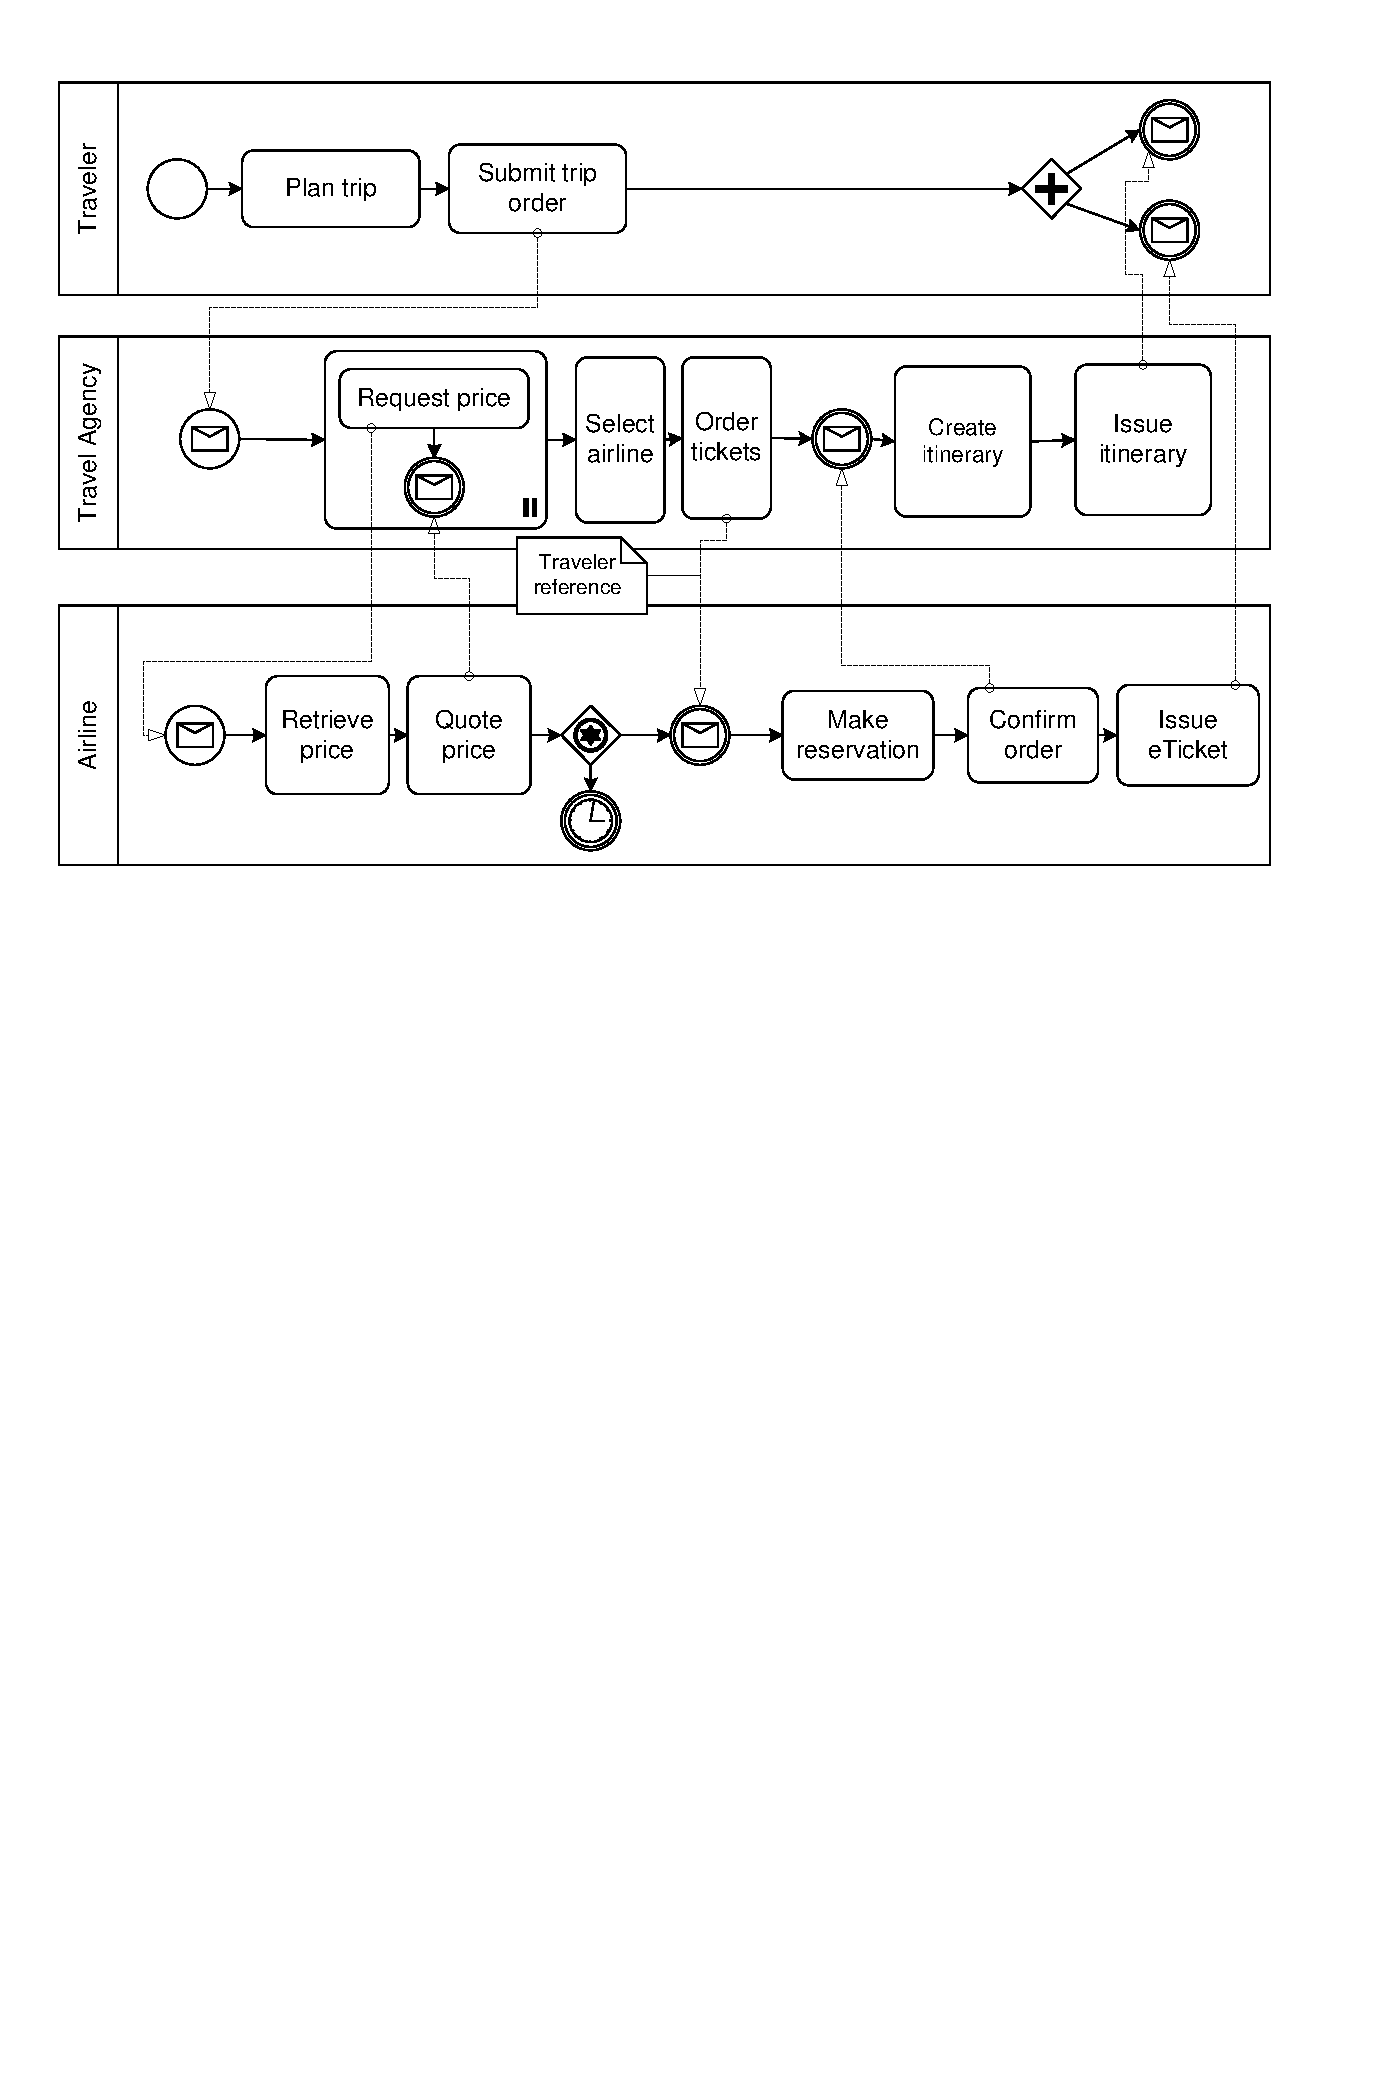
\includegraphics[width=\textwidth]{choreography.pdf}
  \caption{Example Choreography}
  \label{fig:chor1}
\end{figure}

\begin{figure}
  \centering
  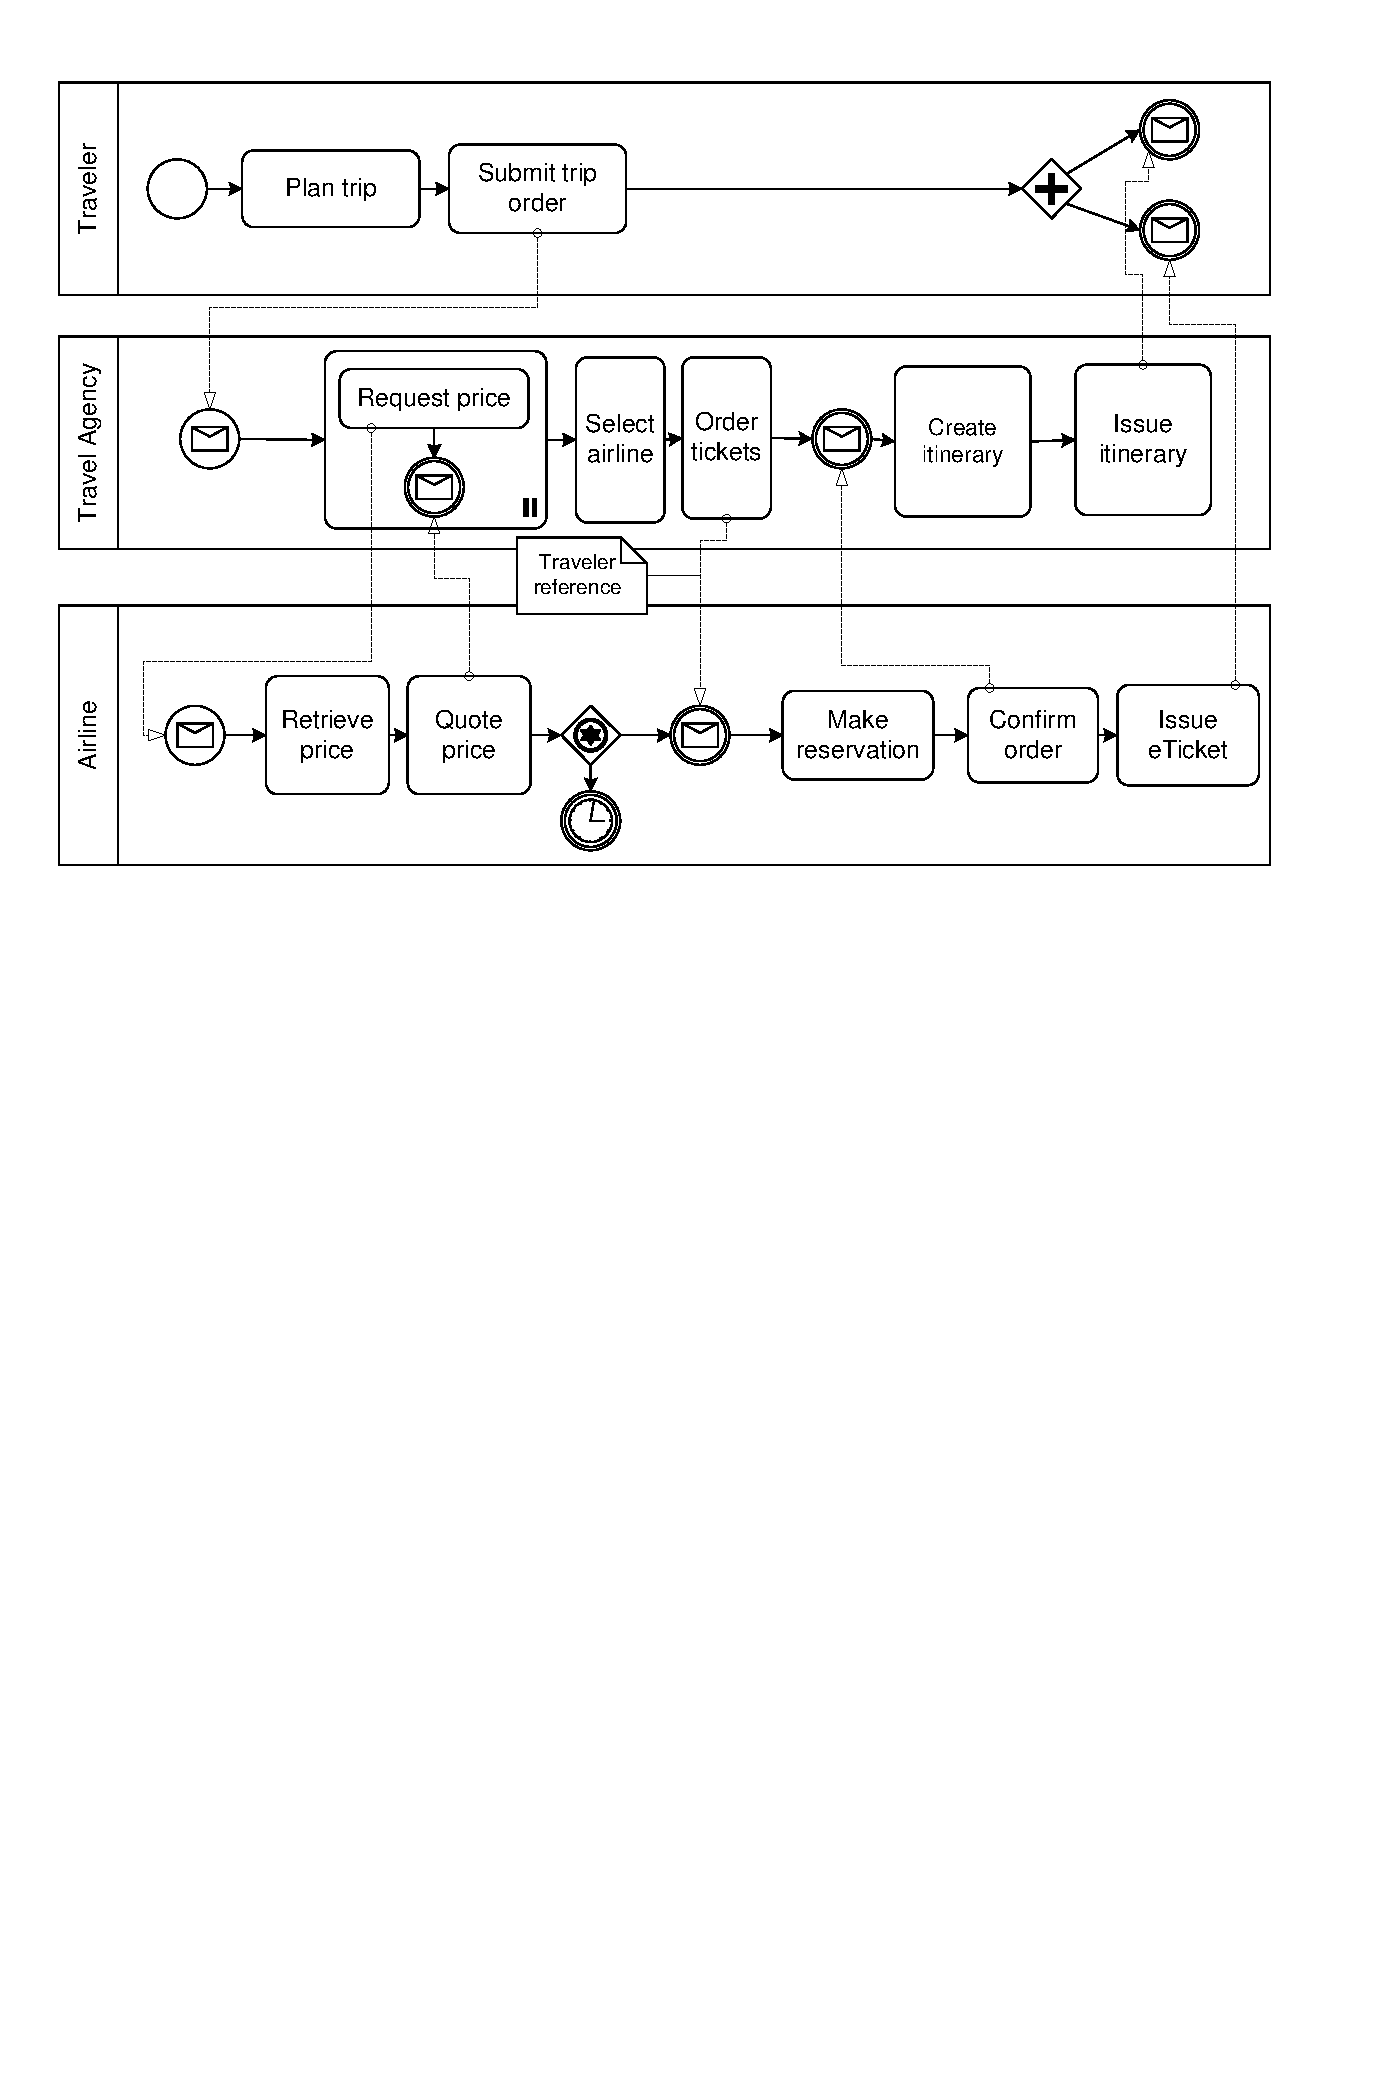
\includegraphics[width=.8\textwidth]{choreography.pdf}
  \caption[Example Choreography]{The example choreography. Now slightly smaller to demonstrate \texttt{\textbackslash textwidth}. And also the use of alternative captions for the list of images. However, the latter is only conditionally recommended, because who reads so much text under a picture? Or is it just a matter of style?}
  \label{fig:chor2}
\end{figure}


\begin{figure}
  \hfill
  \begin{subfigure}{.3\textwidth}
    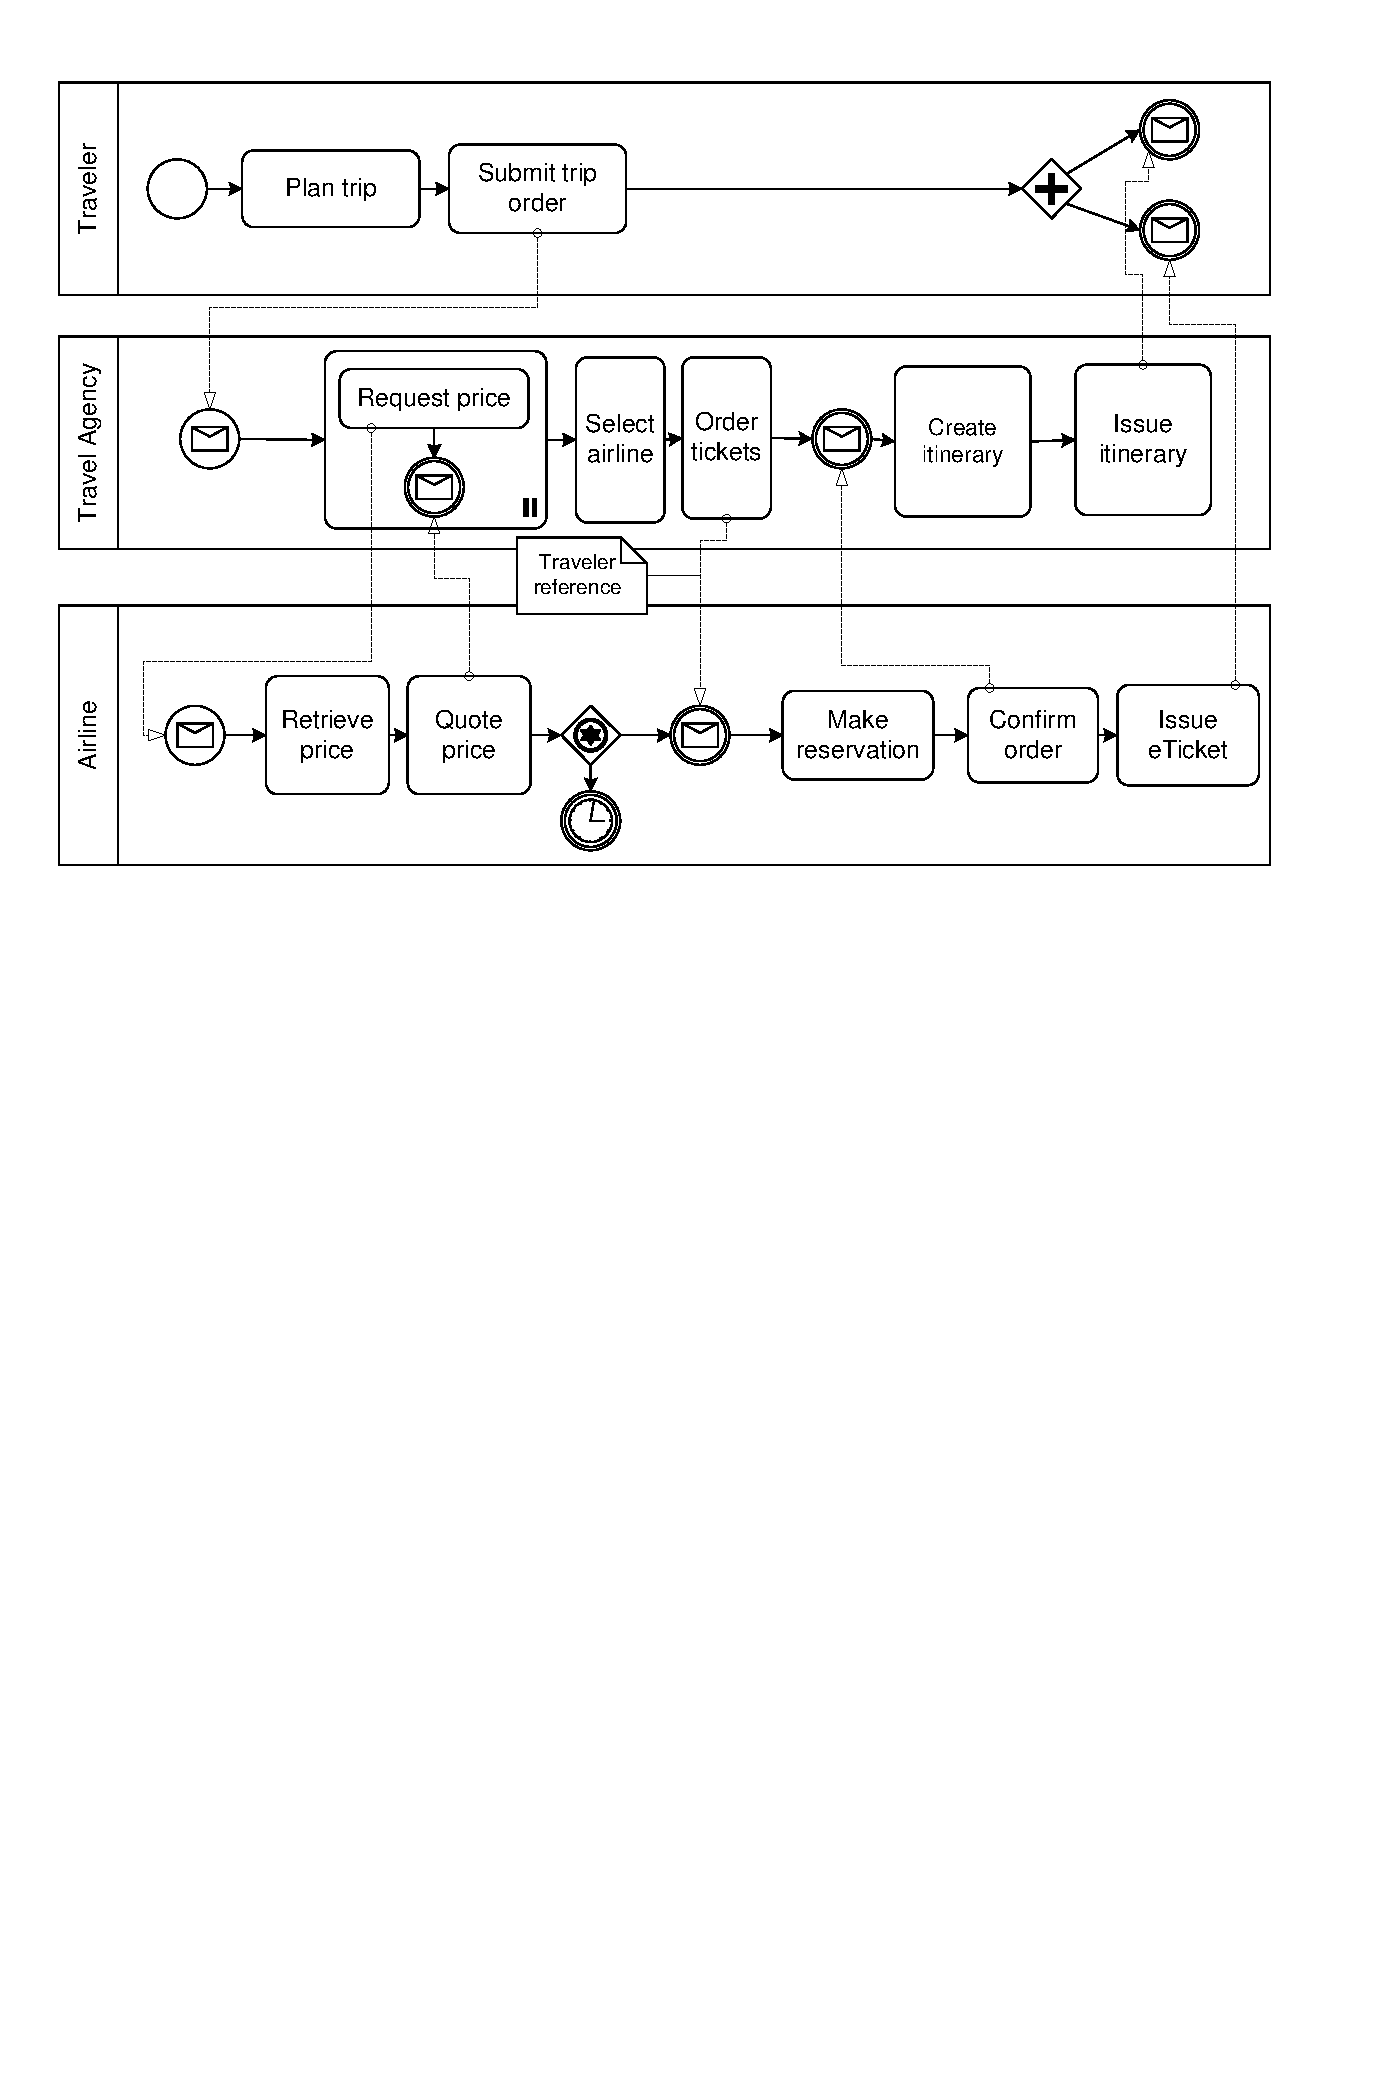
\includegraphics[width=\textwidth]{choreography.pdf}
    \caption{Choreography 1}
    \label{fig:subfigA}
  \end{subfigure}
  \hfill
  \begin{subfigure}{.3\textwidth}
    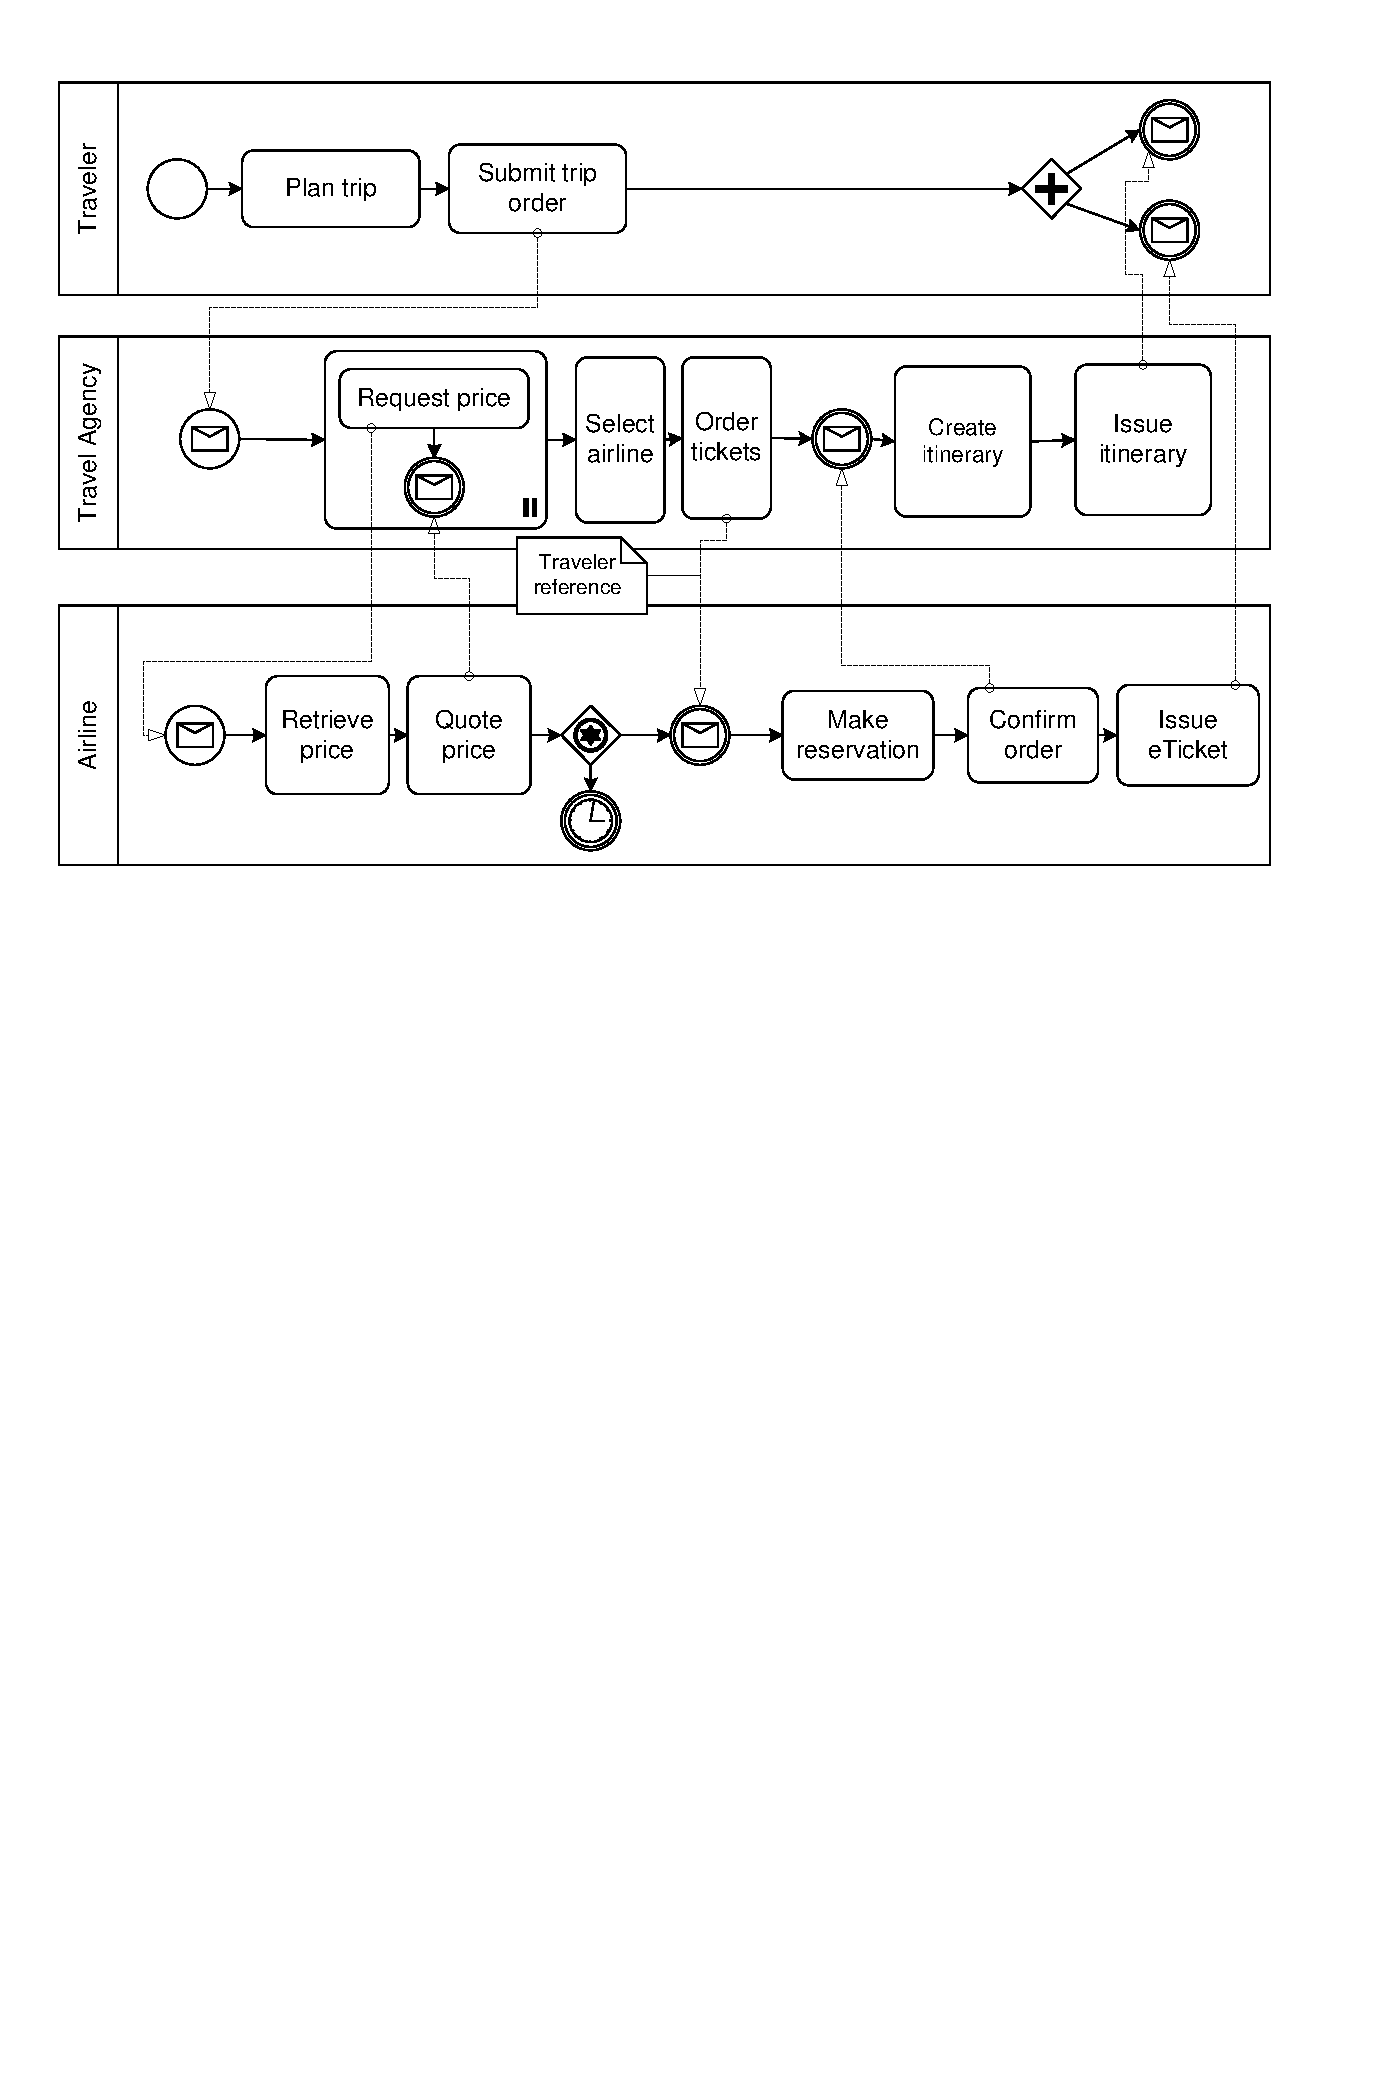
\includegraphics[width=\textwidth]{choreography.pdf}
    \caption{Choreography 2}
    \label{fig:subfigB}
  \end{subfigure}
  \hfill
  \begin{subfigure}{.3\textwidth}
    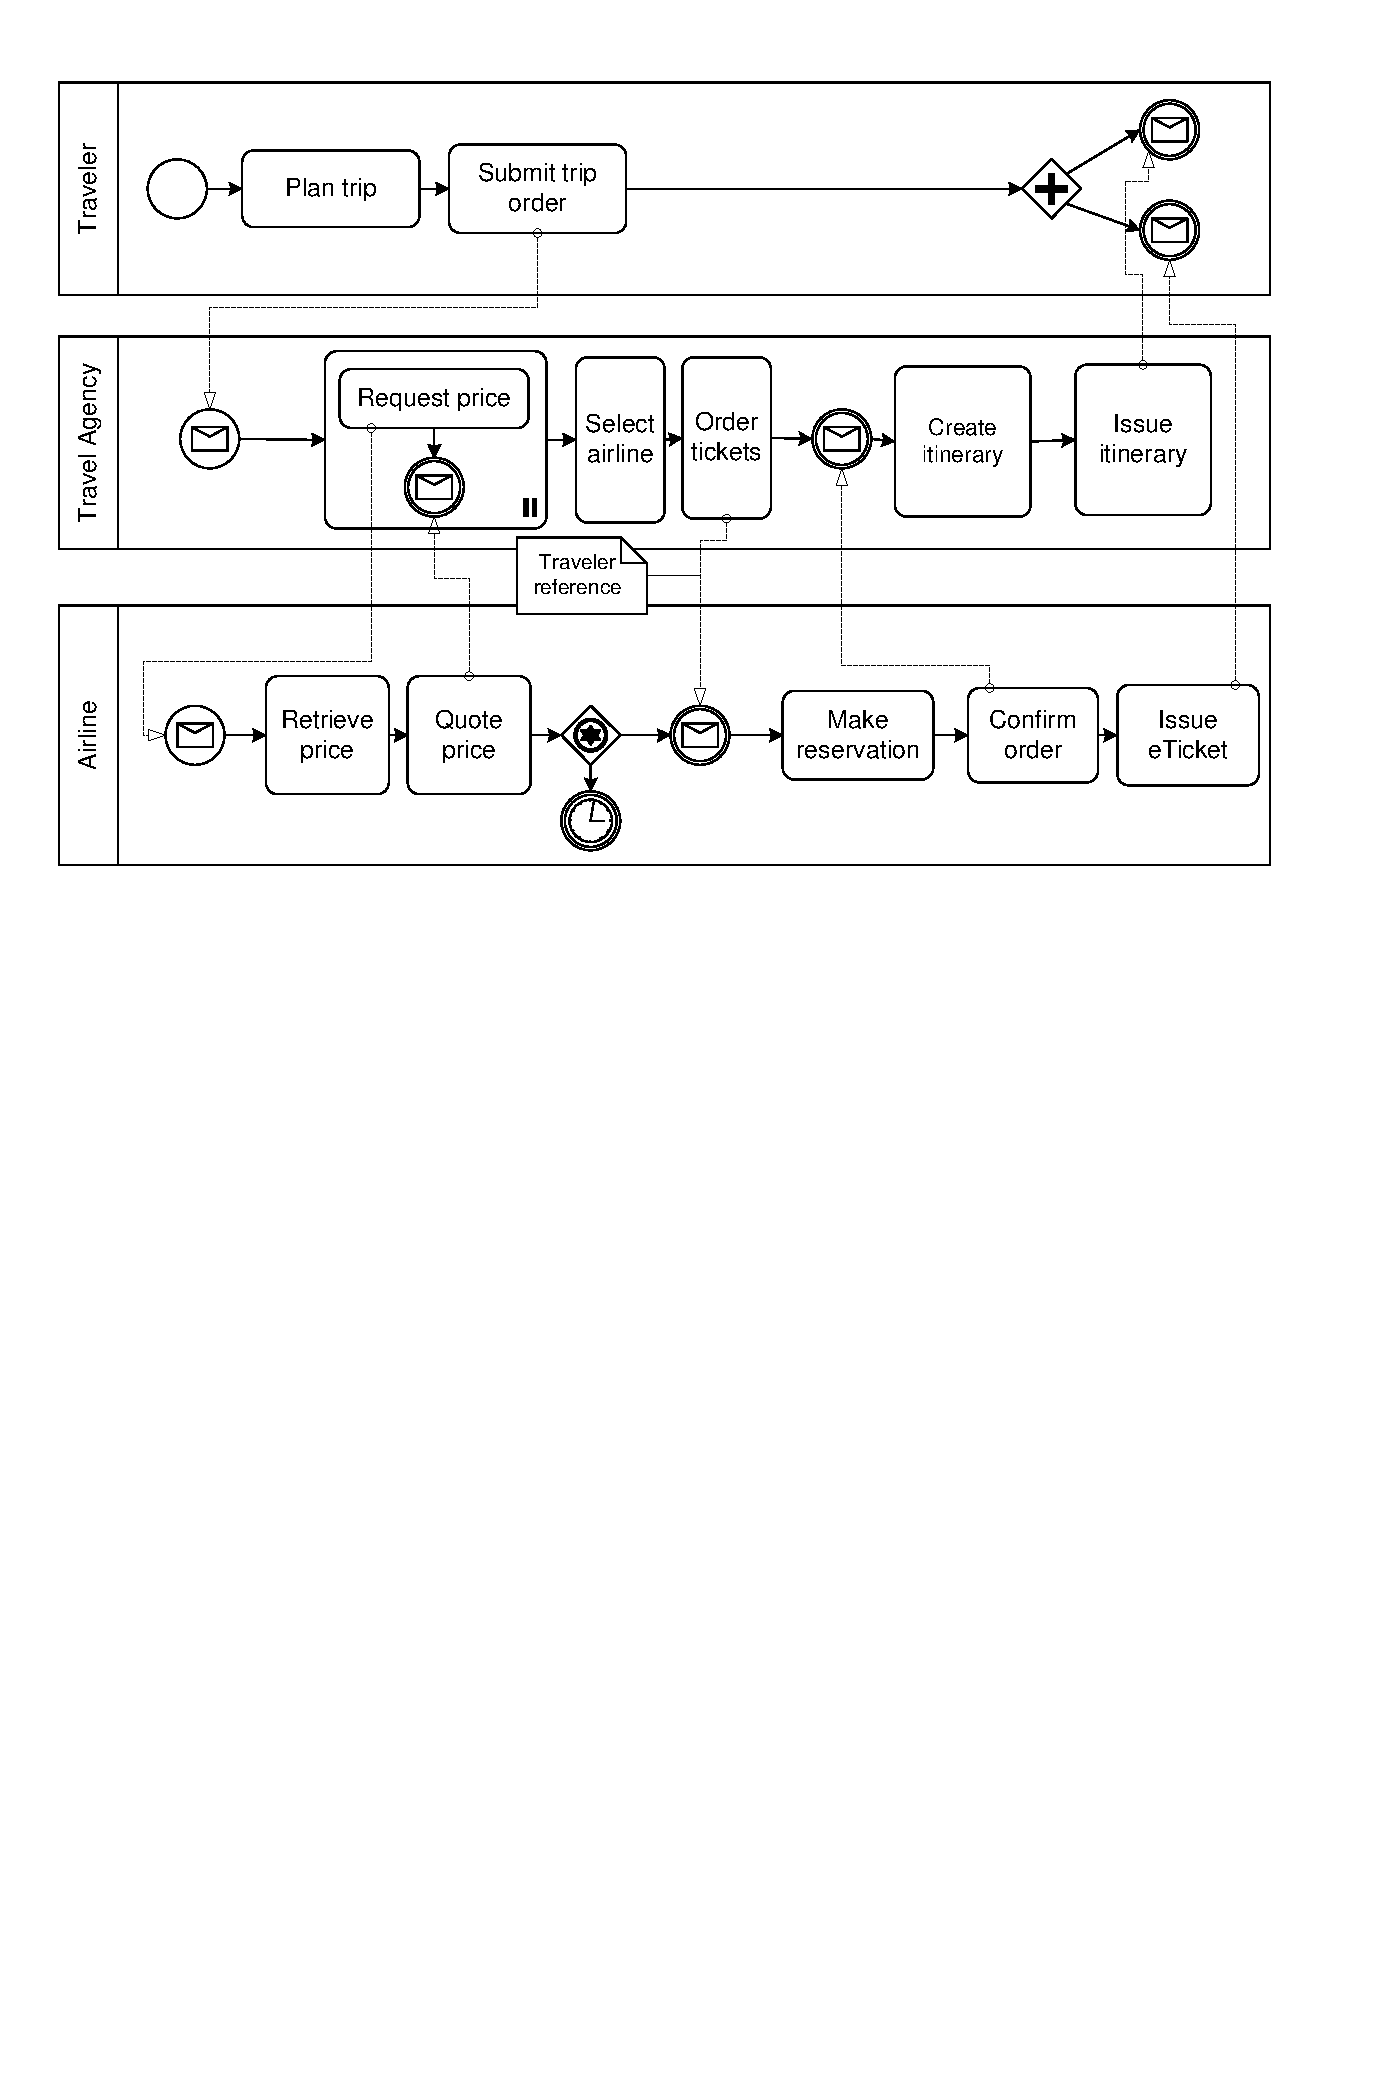
\includegraphics[width=.9\textwidth]{choreography.pdf}
    \caption{Choreography 3}
    \label{fig:subfigC}
  \end{subfigure}
  \caption{Example to place 3 illustrations next to each other. Further, it is possible to reference each separately.}
  \label{fig:subfig_example}
\end{figure}

\Cref{fig:subfig_example} shows the usage of the package subcaption.
It is indeed possible to reference to sub figures: \Cref{fig:subfigA}.

It is possible to convert SVGs to PDF directly during compilation.
This is described in the source code of latex-tipps.tex, but commented out.

\iffalse % <-- Take this away if inkscape is in the path
  The SVG in \cref{fig:directSVG} is directly included, while the text in the SVG in \cref{fig:latexSVG} is set using pdflatex.
  If you want to see the graphics, inkscape must be in PATH and in the text source \texttt{\textbackslash{}iffalse} and \text{\textbackslash{}iftrue} have to be commented out.

  \begin{figure}
    \centering
    
\includegraphics{svgexample.svg}
    \caption{SVG directly included}
    \label{fig:directSVG}
  \end{figure}

  \begin{figure}
    \centering
    \def\svgwidth{.4\textwidth}
    \includesvg{svgexample}
    \caption{Text in SVN set via \LaTeX{}}
    \label{fig:latexSVG}
  \end{figure}
\fi % <-- Take this away if inkscape is in the path



\section{More Illustrations}
\Cref{fig:AnhangsChor,fig:AnhangsChor2} show two choreographies, which should further explain the facts. The second figure is rotated 90 degrees to demonstrate the \texttt{pdflscape} package.

\begin{figure}
  \centering
  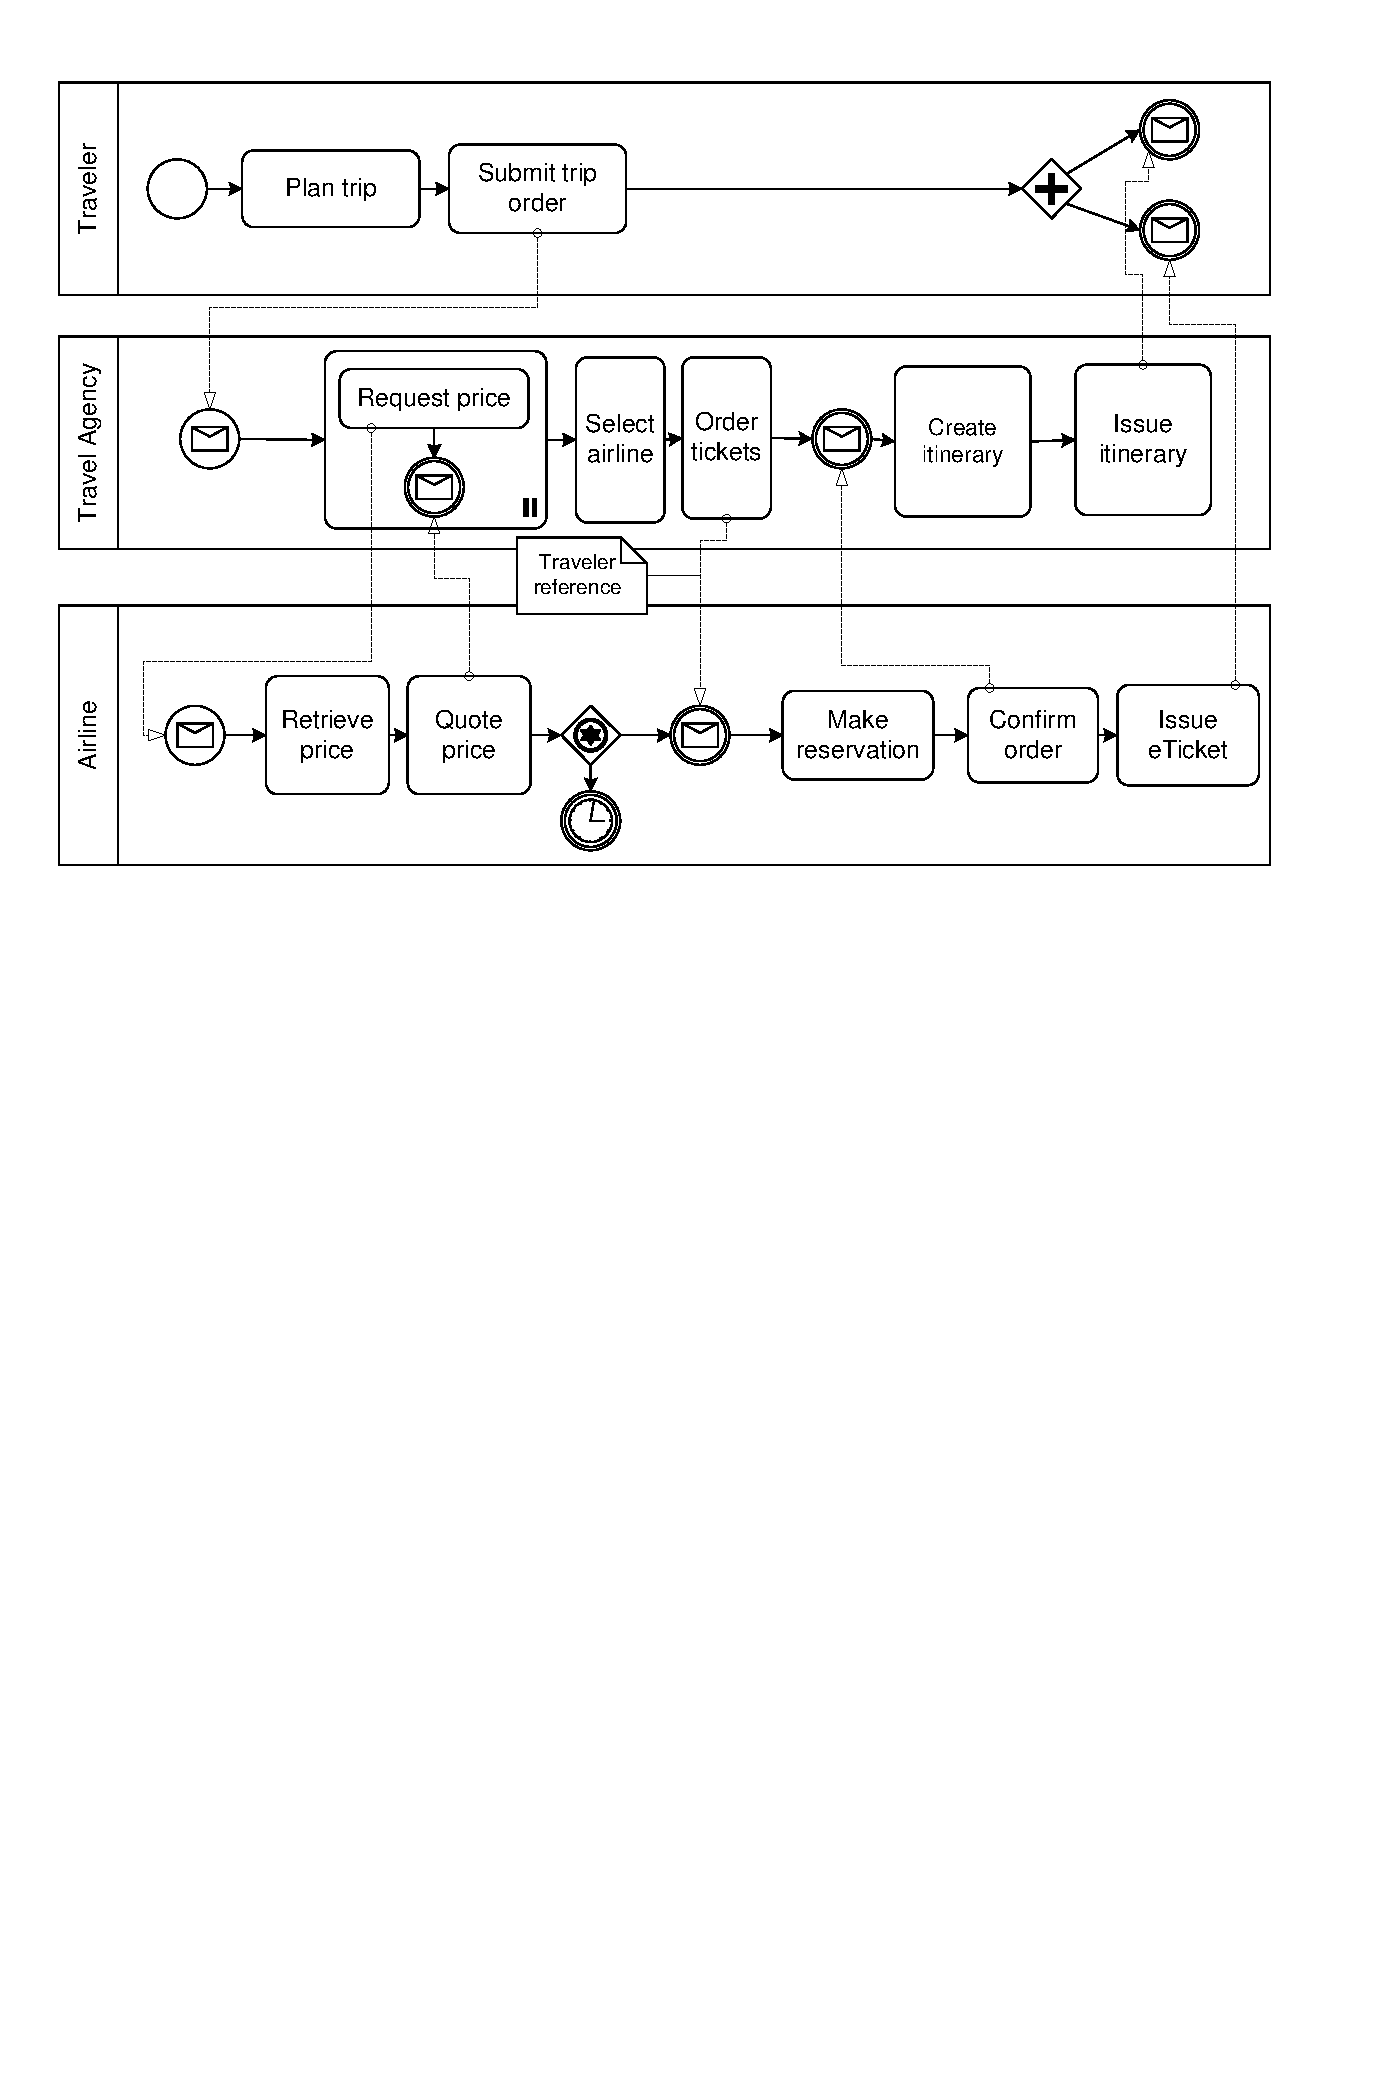
\includegraphics[width=\textwidth]{choreography.pdf}
  \caption{Example Choreography I}
  \label{fig:AnhangsChor}
\end{figure}

\begin{landscape}
  %sidewaysfigure
  \begin{figure}
    \centering
    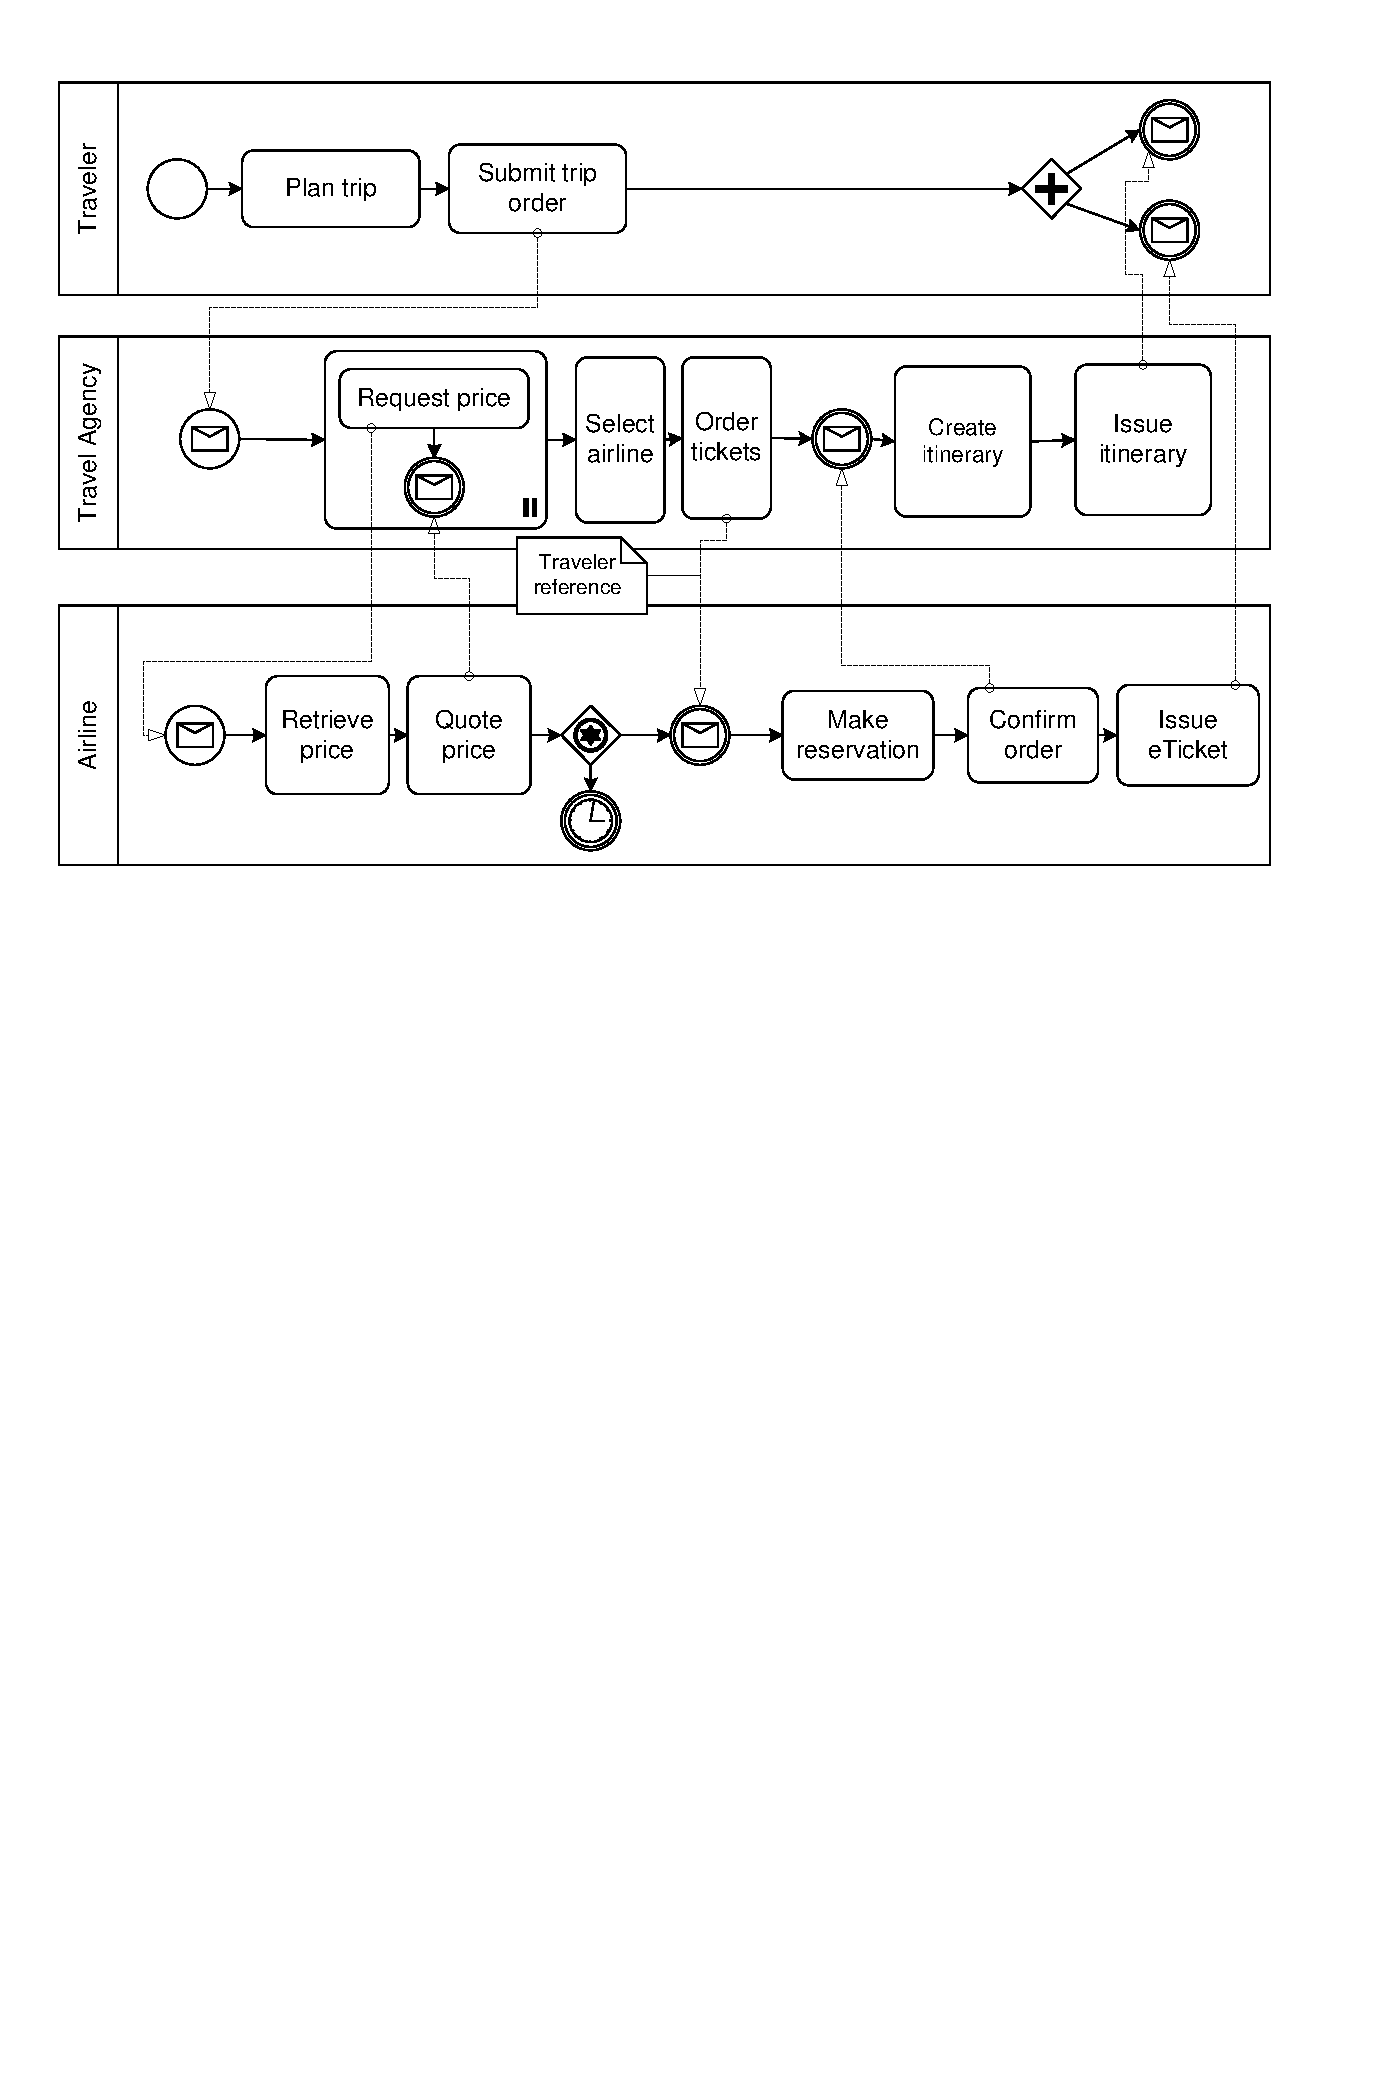
\includegraphics[width=\textwidth]{choreography.pdf}
    \caption{Example Choreography II}
    \label{fig:AnhangsChor2}
  \end{figure}
\end{landscape}


\IfFileExists{pgfplots.sty}{
  %%%%%%%%%%%%%%%%%%%%%%%%%%%%%%%%%%%%%%%%%%%%%%%%%%%%%%%%%%%%%%%%%%%%%%%%%%%%%%
  \section{Plots with pgfplots}
  %%%%%%%%%%%%%%%%%%%%%%%%%%%%%%%%%%%%%%%%%%%%%%%%%%%%%%%%%%%%%%%%%%%%%%%%%%%%%%
  The package pdfplots provides plotting of functions directly in \LaTeX~like with matlab or gnuplot. Some visual examples are available here\footnote{\url{http://texdoc.net/pkg/visualtikz}}.
  \begin{figure}[h]
    \centering
    \begin{tikzpicture}
      \begin{axis}[xlabel=$x$,
          ylabel=$\sin(x)$]
        \addplot {sin(deg(x))};  % Print sine function
      \end{axis}
    \end{tikzpicture}
    \caption{Plot of $\sin(x)$ direclty inside the figure environment with pgfplots.}
  \end{figure}

  \begin{figure}[h]
    \centering
    \begin{tikzpicture}
      \begin{axis}[xlabel=$x$,
          ylabel=$y$]
        \addplot table [x=a, y=c, col sep=comma] {data/data.csv};  % Read coordinates from csv file and plot them
      \end{axis}
    \end{tikzpicture}
    \caption{Coordinates $x$ and $y$ read from csv file and plotted pgfplots.}
  \end{figure}

}{}


%%%%%%%%%%%%%%%%%%%%%%%%%%%%%%%%%%%%%%%%%%%%%%%%%%%%%%%%%%%%%%%%%%%%%%%%%%%%%%
\section{Figures with tikz}
%%%%%%%%%%%%%%%%%%%%%%%%%%%%%%%%%%%%%%%%%%%%%%%%%%%%%%%%%%%%%%%%%%%%%%%%%%%%%%
The tikz is a package for creating graphics programmatically. With this package grids or other regular strucutres can be easliy generated.

\begin{figure}[ht]
  \centering
  \begin{tikzpicture}
    \draw(0,0) rectangle (4,4);
    \foreach \x in {0.5,1,1.5,2,2.5,3,3.5}
    \foreach \y in {0.5,1,1.5,2,2.5,3,3.5}
    \draw(\x,\y) circle (1pt);
  \end{tikzpicture}
  \caption{A regular grid genrated with easily with two for loops.}\label{fig:tikz_example}
\end{figure}


%%%%%%%%%%%%%%%%%%%%%%%%%%%%%%%%%%%%%%%%%%%%%%%%%%%%%%%%%%%%%%%%%%%%%%%%%%%%%%
\section{UML diagrams using tikz-uml}
%%%%%%%%%%%%%%%%%%%%%%%%%%%%%%%%%%%%%%%%%%%%%%%%%%%%%%%%%%%%%%%%%%%%%%%%%%%%%%

\Cref{fig:uml} presents a class diagram typeset using tikz-uml.

\begin{figure}
  \centering
  \begin{tikzpicture}
  \begin{umlpackage}{p}
  \begin{umlpackage}{sp1}
  \umlclass[template=T]{A}{
    n : uint \\ t : float
  }{}
  \umlclass[y=-3]{B}{
    d : double
  }{
    \umlvirt{setB(b : B) : void} \\ getB() : B}
  \end{umlpackage}
  \begin{umlpackage}[x=10,y=-6]{sp2}
  \umlinterface{C}{
    n : uint \\ s : string
  }{}
  \end{umlpackage}
  \umlclass[x=2,y=-10]{D}{
    n : uint
    }{}
  \end{umlpackage}

  \umlassoc[geometry=-|-, arg1=tata, mult1=*, pos1=0.3, arg2=toto, mult2=1, pos2=2.9, align2=left]{C}{B}
  \umlunicompo[geometry=-|, arg=titi, mult=*, pos=1.7, stereo=vector]{D}{C}
  \umlimport[geometry=|-, anchors=90 and 50, name=import]{sp2}{sp1}
  \umlaggreg[arg=tutu, mult=1, pos=0.8, angle1=30, angle2=60, loopsize=2cm]{D}{D}
  \umlinherit[geometry=-|]{D}{B}
  \umlnote[x=2.5,y=-6, width=3cm]{B}{A note with respect to class B}
  \umlnote[x=7.5,y=-2]{import-2}{A anotation}
  \end{tikzpicture}
  \caption{Class diagram generated with tikz-uml. Example adapted from Nicolas Kielbasiewicz.}
  \label{fig:uml}
\end{figure}

\section{UML diagrams using PlantUML}

In case \lualatex{} is used and PlantUML is installed, UML diagrams can be defined using PlantUML.

% Only works if "--shell-escape" is activated. Please activate only if you are sure, your compilation settings are correct
%\IfFileExists{plantuml.sty}{\input{latexhints-english-plantuml}}{}


%%%%%%%%%%%%%%%%%%%%%%%%%%%%%%%%%%%%%%%%%%%%%%%%%%%%%%%%%%%%%%%%%%%%%%%%%%%%%%
\section{Linguistic Forests}
%%%%%%%%%%%%%%%%%%%%%%%%%%%%%%%%%%%%%%%%%%%%%%%%%%%%%%%%%%%%%%%%%%%%%%%%%%%%%%

\begin{filecontents*}{\democodefile}
\begin{forest}
  [VP
    [DP]
    [V’
      [V]
      [DP]
    ]
  ]
\end{forest}
\end{filecontents*}
\PrintDemo{style=parallel}


%%%%%%%%%%%%%%%%%%%%%%%%%%%%%%%%%%%%%%%%%%%%%%%%%%%%%%%%%%%%%%%%%%%%%%%%%%%%%%
\section{Tables}
%%%%%%%%%%%%%%%%%%%%%%%%%%%%%%%%%%%%%%%%%%%%%%%%%%%%%%%%%%%%%%%%%%%%%%%%%%%%%%
\cref{tab:Ergebnisse} shows results and \cref{tab:Werte} shows how numerical data can be represented in a table.
\begin{table}
  \centering
  \begin{tabular}{ccc}
    \toprule
    \multicolumn{2}{c}{\textbf{summed}} & \textbf{Title}                                                          \\ \midrule
    Table                                      & as                                                           & in      \\
    \url{tabsatz.pdf}                            & recommended                                                     & gesetzt \\

    \multirow{2}{*}{Example}                    & \multicolumn{2}{c}{a nice example}                                \\
                                                 & \multicolumn{2}{c}{for using \qq{multirow}}           \\
    \bottomrule
  \end{tabular}
  \caption[Example Table]{Exampe Table -- see \url{http://www.ctan.org/tex-archive/info/german/tabsatz/}}
  \label{tab:Ergebnisse}
\end{table}

\begin{table}
  \centering
  \begin{tabular}{l *{8}{d{3.2}}}
    \toprule

                         & \multicolumn{2}{c}{\textbf{Parameter 1}} & \multicolumn{2}{c}{\textbf{Parameter 2}} & \multicolumn{2}{c}{\textbf{Parameter 3}} & \multicolumn{2}{c}{\textbf{Parameter 4}}                                                                                                                                       \\
    \cmidrule(r){2-3}\cmidrule(lr){4-5}\cmidrule(lr){6-7}\cmidrule(l){8-9}

    \textbf{Bedingungen} & \multicolumn{1}{c}{\textbf{M}}           & \multicolumn{1}{c}{\textbf{SD}}          & \multicolumn{1}{c}{\textbf{M}}           & \multicolumn{1}{c}{\textbf{SD}}          & \multicolumn{1}{c}{\textbf{M}} & \multicolumn{1}{c}{\textbf{SD}} & \multicolumn{1}{c}{\textbf{M}} & \multicolumn{1}{c}{\textbf{SD}} \\
    \midrule

    W                    & 1.1                                      & 5.55                                     & 6.66                                     & .01                                      &                                &                                 &                                &                                 \\
    X                    & 22.22                                    & 0.0                                      & 77.5                                     & .1                                       &                                &                                 &                                &                                 \\
    Y                    & 333.3                                    & .1                                       & 11.11                                    & .05                                      &                                &                                 &                                &                                 \\
    Z                    & 4444.44                                  & 77.77                                    & 14.06                                    & .3                                       &                                &                                 &                                &                                 \\
    \bottomrule
  \end{tabular}

  \caption{Example table for 4 constraints (W-Z), each having 4 parameters with (M und SD). Note: use always the same number of decimal places.}
  \label{tab:Werte}
\end{table}

\IfFileExists{pgfplotstable.sty}{

\subsection{Tables with pgfplots}
With the pgfplotstable package tables can be directly generated from a csv file.

\begin{table}[h]
\centering
\pgfplotstabletypeset[
col sep = comma,
every head row/.style={before row=\toprule,after row=\midrule},
every last row/.style={after row=\bottomrule},
display columns/0/.style={string type,column name={}}
]
{data/data.csv}
\caption{Table direclty generated from the values of a csf file.}
\end{table}
}{}


\section{Tables spanning multiple pages}


\begin{longtable}{|l|l|l|}
\caption{A sample long table.} \label{tab:long} \\

\hline \multicolumn{1}{|c|}{\textbf{First column}} & \multicolumn{1}{c|}{\textbf{Second column}} & \multicolumn{1}{c|}{\textbf{Third column}} \\ \hline
\endfirsthead

\multicolumn{3}{c}%
{{\bfseries \tablename\ \thetable{} -- continued from previous page}} \\
\hline \multicolumn{1}{|c|}{\textbf{First column}} & \multicolumn{1}{c|}{\textbf{Second column}} & \multicolumn{1}{c|}{\textbf{Third column}} \\ \hline
\endhead

\hline \multicolumn{3}{|r|}{{Continued on next page}} \\ \hline
\endfoot

\hline \hline
\endlastfoot

A & BC & D \\
A & BC & D \\
A & BC & D \\
A & BC & D \\
A & BC & D \\
A & BC & D \\
A & BC & D \\
A & BC & D \\
A & BC & D \\
A & BC & D \\
A & BC & D \\
A & BC & D \\
A & BC & D \\
A & BC & D \\
A & BC & D \\
A & BC & D \\
A & BC & D \\
A & BC & D \\
A & BC & D \\
A & BC & D \\
A & BC & D \\
A & BC & D \\
A & BC & D \\
A & BC & D \\
A & BC & D \\
A & BC & D \\
A & BC & D \\
A & BC & D \\
A & BC & D \\
A & BC & D \\
A & BC & D \\
A & BC & D \\
A & BC & D \\
A & BC & D \\
A & BC & D \\
A & BC & D \\
A & BC & D \\
A & BC & D \\
A & BC & D \\
A & BC & D \\
A & BC & D \\
A & BC & D \\
A & BC & D \\
A & BC & D \\
A & BC & D \\
A & BC & D \\
A & BC & D \\
A & BC & D \\
A & BC & D \\
A & BC & D \\
A & BC & D \\
A & BC & D \\
A & BC & D \\
A & BC & D \\
A & BC & D \\
A & BC & D \\
A & BC & D \\
A & BC & D \\
A & BC & D \\
A & BC & D \\
A & BC & D \\
A & BC & D \\
A & BC & D \\
A & BC & D \\
A & BC & D \\
A & BC & D \\
A & BC & D \\
A & BC & D \\
A & BC & D \\
A & BC & D \\
A & BC & D \\
A & BC & D \\
A & BC & D \\
A & BC & D \\
A & BC & D \\
A & BC & D \\
A & BC & D \\
A & BC & D \\
A & BC & D \\
A & BC & D \\
\end{longtable}


%%%%%%%%%%%%%%%%%%%%%%%%%%%%%%%%%%%%%%%%%%%%%%%%%%%%%%%%%%%%%%%%%%%%%%%%%%%%%%
\section{Abbreviations}
%%%%%%%%%%%%%%%%%%%%%%%%%%%%%%%%%%%%%%%%%%%%%%%%%%%%%%%%%%%%%%%%%%%%%%%%%%%%%%
At the first pass the \gls{fr} was 5.
At the second pass was \gls{fr} 3.
The plural form can be seen here: \glspl{er}.
To demonstrate what the list of abbreviations looks like for longer description texts, \glspl{rdbms} must be mentioned here.

With \verb+\gls{...}+ you can enter abbreviations, the first time you call it, the long form is used.
When reusing \verb+\gls{..}+ the short form is automatically displayed.
The abbreviation is also automatically inserted in the abbreviation list.
With \verb+\glspl{...}+ the plural form is used.
If you want the short form to appear directly at the first use, you can use \verb+\glsunset{..}+ to mark an abbreviation as already used.
The opposite is achieved with \verb+\glsreset{..}+.

Abbreviations are defined in \verb+\content\ausarbeitung.tex+ by means of \verb+\newacronym{...}{...}{...}+.

More information at: \url{http://tug.ctan.org/macros/latex/contrib/glossaries/glossariesbegin.pdf}
%%%%%%%%%%%%%%%%%%%%%%%%%%%%%%%%%%%%%%%%%%%%%%%%%%%%%%%%%%%%%%%%%%%%%%%%%%%%%%
\section{References}
%%%%%%%%%%%%%%%%%%%%%%%%%%%%%%%%%%%%%%%%%%%%%%%%%%%%%%%%%%%%%%%%%%%%%%%%%%%%%%
For distant sections \qq{varioref} is recommended:
\qq{See \vref{sec:mf}}.
The command \texttt{\textbackslash{}vref} works similar to \texttt{\textbackslash{}cref} the difference beeing that a reference to the page is additionally added.
\texttt{vref}: \qq{\vref{sec:firstsectioninlatexhints}}, \texttt{cref}: \qq{\cref{sec:firstsectioninlatexhints}}, \texttt{ref}: \qq{\ref{sec:firstsectioninlatexhints}}.

If \qq{varioref} causes difficulties, then \qq{cref} can be used instead.
This also creates the word \qq{section} automatically: \cref{sec:mf}.
This is also possible for illustrations etc.
In English please use \verb1\Cref{...}1 (with large \qq{C} at the beginning).

%With MiKTeX installation from 2012-01-16 no longer necessary.
%If a section becomes longer than one page and you want to refer to a specific place in the section with \texttt{\textbackslash{}vref}, then you should use \texttt{\textbackslash{}phantomsection} then using \texttt{vref} will also display the correct page number.

%%The link location will be placed on the line below.
%%Tipp von http://en.wikibooks.org/wiki/LaTeX/Labels_and_Cross-referencing#The_hyperref_package_and_.5Cphantomsection
%\phantomsection
%\label{alabel}
%View the example for \texttt{\textbackslash{}phantomsection} in the \LaTeX{} source code.

%Here is the example: See Section \vref{hack1} and Section \vref{hack2}.
%%%%%%%%%%%%%%%%%%%%%%%%%%%%%%%%%%%%%%%%%%%%%%%%%%%%%%%%%%%%%%%%%%%%%%%%%%%%%%
\section{Definitions}
%%%%%%%%%%%%%%%%%%%%%%%%%%%%%%%%%%%%%%%%%%%%%%%%%%%%%%%%%%%%%%%%%%%%%%%%%%%%%%
\begin{definition}[Title]
  \label{def:def1}
  Definition Text
\end{definition}

\Cref{def:def1} shows \ldots

%%%%%%%%%%%%%%%%%%%%%%%%%%%%%%%%%%%%%%%%%%%%%%%%%%%%%%%%%%%%%%%%%%%%%%%%%%%%%%
\section{Footnotes}
%%%%%%%%%%%%%%%%%%%%%%%%%%%%%%%%%%%%%%%%%%%%%%%%%%%%%%%%%%%%%%%%%%%%%%%%%%%%%%
Footnotes are provided by the command \verb+\footnote{...}+\footnote{\label{fussnote}Example footnote.}. Citing footnotes is possible by provinding a label\verb+\footnote{\label{...}...}+ and cite the footnote with \verb+\cref{...}+ in the text\cref{fussnote}.
%%%%%%%%%%%%%%%%%%%%%%%%%%%%%%%%%%%%%%%%%%%%%%%%%%%%%%%%%%%%%%%%%%%%%%%%%%%%%%

%%%%%%%%%%%%%%%%%%%%%%%%%%%%%%%%%%%%%%%%%%%%%%%%%%%%%%%%%%%%%%%%%%%%%%%%%%%%%%
\section{Various Things}
%%%%%%%%%%%%%%%%%%%%%%%%%%%%%%%%%%%%%%%%%%%%%%%%%%%%%%%%%%%%%%%%%%%%%%%%%%%%%%
\label{sec:diff}
\ifdeutsch
  Numbers (123\,654\,789) are nicely set.
  Either in a line or as non-lining figure.
  The latter is reached by parameter \texttt{osf} at package \texttt{libertine} or.\ \texttt{mathpazo} in \text{fonts.tex}.
\fi

\begin{filecontents*}{\democodefile}
\begin{compactenum}[I.]
  \item You can also keep the numbering compact thanks to paralist
  \item and switch to a different numbering
\end{compactenum}
\end{filecontents*}
\PrintDemo{style=parallel}

The words \qq{workflow} and \qq{dwarflike} can be copied from the PDF and pasted to a text file.

\begin{filecontents*}{\democodefile}
In case \LuaLaTeX{} is used as compiler, there is no ligature at \qq{f\/l} in the word \qq{dwarflike} (in contrast to \qq{fl} at \qq{workflow}).
In other words: \qq{dwarflike} and \qq{dwarf\/like} look the same in the PDF.
In case they do not, there is an issue with Lua\LaTeX{} and the selnolig package.
\end{filecontents*}
\PrintDemo{style=parallel}
% Meta comment: The precise form of the optimal ligation suppression command may vary depending on the character pairs involved - see https://tex.stackexchange.com/q/28437/9075


%%%%%%%%%%%%%%%%%%%%%%%%%%%%%%%%%%%%%%%%%%%%%%%%%%%%%%%%%%%%%%%%%%%%%%%%%%%%%%
\section{Closing remarks}
%%%%%%%%%%%%%%%%%%%%%%%%%%%%%%%%%%%%%%%%%%%%%%%%%%%%%%%%%%%%%%%%%%%%%%%%%%%%%%
Please feel free to provide enhancements for this template and create a new ticket on GitHub (\url{https://github.com/latextemplates/uni-stuttgart-computer-science-template/issues}).

\pagestyle{empty}
\renewcommand*{\chapterpagestyle}{empty}
\Affirmation
\end{document}
